\documentclass[a4paper]{article}

%Tutti gli usepackage vanno qui

\usepackage{geometry}
\usepackage[italian]{babel}
\usepackage[utf8]{inputenc}
\usepackage[T1]{fontenc}
\usepackage{tgschola}
%\usepackage{tgbonum}
\usepackage{tabularx}
\usepackage{longtable}
\usepackage{hyperref}
\usepackage{enumitem}
\usepackage[toc]{appendix}
\hypersetup{
	colorlinks=true,
	linkcolor=black,
	filecolor=magenta,      
	urlcolor=blue,
}
% Numerazione figure 
\let\counterwithout\relax
\let\counterwithin\relax
\usepackage{chngcntr}

\counterwithin{table}{subsection}
\counterwithin{figure}{subsection}

\usepackage[bottom]{footmisc}
\usepackage{fancyhdr}
\setcounter{secnumdepth}{4}
\usepackage{amsmath, amssymb}
\usepackage{array}
\usepackage{graphicx}

\usepackage{ifthen}

%\usepackage{float}
\usepackage{layouts}
\usepackage{url}
\usepackage{comment}
\usepackage{float}
\usepackage{eurosym}

\usepackage{lastpage}
\usepackage{layouts}
\usepackage{float}
\usepackage{eurosym}

%Comandi di impaginazione uguale per tutti i documenti
\pagestyle{fancy}
\lhead{
\includegraphics[scale=0.04]{../../../../latex/images/logoTWM.png}}
%Titolo del documento
\rhead{\doctitle{}}
%\rfoot{\thepage}
\cfoot{Pagina \thepage\ di \pageref{LastPage}}
\setlength{\headheight}{35pt}
\setcounter{tocdepth}{5}
\setcounter{secnumdepth}{5}
\renewcommand{\footrulewidth}{0.4pt}

% multirow per tabelle
\usepackage{multirow}

% Permette tabelle su più pagine
%\usepackage{longtable}


% colore di sfondo per le celle
\usepackage[table]{xcolor}

%COMANDI TABELLE
\newcommand{\rowcolorhead}{\rowcolor[HTML]{9b240a}} %intestazione 
% check for missing commands
\newcommand{\headertitle}[1]{\textbf{\color{white}#1}} %titolo colonna
\definecolor{pari}{HTML}{FFDBCB}
\definecolor{dispari}{HTML}{F1F7FD}

% comandi glossario
\newcommand{\glo}{$_{G}$}
\newcommand{\glosp}{$_{G}$ }


%label custom
\makeatletter
\newcommand{\uclabel}[2]{%
	\protected@write \@auxout {}{\string \newlabel {#1}{{#2}{\thepage}{#2}{#1}{}} }%
	\hypertarget{#1}{#2}
}
\makeatother

%riportare pezzi di codice
\definecolor{codegray}{gray}{0.9}
\newcommand{\code}[1]{\colorbox{codegray}{\texttt{#1}}}



% Configurazione della pagina iniziale
\newcommand{\doctitle}{Norme di Progetto}
\newcommand{\docdate}{ } % lasciare vuoto (uno carattere di spazio) per i documenti che non sono verbali, così non viene scritta la data
\newcommand{\rev}{3.0.1}
\newcommand{\stato}{Non Approvato}
\newcommand{\uso}{Interno}
\newcommand{\approv}{--De Renzis Simone}
\newcommand{\red}{Greggio Nicolò\\& Tessari Andrea}
\newcommand{\ver}{Zuccolo Giada\\& Crivellari Alberto}
\newcommand{\dest}{Three Way Milkshake\\ Prof. Vardanega Tullio\\ Prof.
 Cardin Riccardo}
\newcommand{\describedoc}{Questo documento contiene tutte le norme di progetto\textsubscript{G}, definite inizialmente o aggiunte in seguito, viene quindi aggiornato per incrementi successivi.}



 % modifica questo file
\makeindex

\usepackage{hyperref}
\usepackage{ulem}
\usepackage{listings}
\usepackage{float}

\begin{document}
	\thispagestyle{empty}
\begin{titlepage}
	\begin{center}
		
		
\includegraphics[scale = 0.17]{../../../../latex/images/logoTWM.png}\\[0.7cm]
		

		\noindent\rule{\textwidth}{1pt} \\[0.4cm]
		\Huge \textbf{\doctitle} \\[0.1cm]
		\ifthenelse{\equal{\docdate}{ }}{ }{ \huge \textbf{\docdate} \\[0.1cm] }
		
		\noindent\rule{\textwidth}{1pt}\\[0.7cm]
		
		\large \textbf{Three Way Milkshake - Progetto "PORTACS"} \\[0.4cm] 
                \texttt{threewaymilkshake@gmail.com} \\[0.4cm]
                
		
        
        
        \large

        \begin{tabular}{r|l}
                        \textbf{Versione} & \rev{} \\
                        \textbf{Stato} & \stato{} \\
                        \textbf{Uso} & \uso{} \\                         
                        \textbf{Approvazione} & \approv{} \\                      
                        \textbf{Redazione} & \red{} \\ 
                        \textbf{Verifica} &  \ver{} \\                         
                        \textbf{Destinatari} & \parbox[t]{5cm}{ \dest{} }
                \end{tabular} 
                \\[0.3cm]
                \large \textbf{Descrizione} \\ \describedoc{} 
               

	\end{center}
\end{titlepage}
	\pagebreak

	% Registro delle modifiche
	\section*{Registro delle modifiche}

\newcommand{\changelogTable}[1]{
	
	
	\renewcommand{\arraystretch}{1.5}
	\rowcolors{2}{pari}{dispari}
	\begin{longtable}{ 
			>{\centering}p{0.07\textwidth} 
			>{}p{0.21\textwidth}
			>{\centering}p{0.17\textwidth}
			>{\centering}p{0.13\textwidth} 
			>{\centering}p{0.17\textwidth} 
			>{\centering}p{0.13\textwidth} }
		\rowcolorhead
		\headertitle{Vers.} &
		\centering \headertitle{Descrizione} &	
		\headertitle{Redazione} &
		\headertitle{Data red.} & 
		\headertitle{Verifica} &
		\headertitle{Data ver.}
		\endfirsthead	
		\endhead
		
		#1
		
	\end{longtable}
	\vspace{-2em}
	
}


\newcommand{\approvingTable}[1]{ 
	
	
	\renewcommand{\arraystretch}{1.5}
	\rowcolors{2}{pari}{dispari}
	\begin{longtable}{ 
			>{\centering}p{0.07\textwidth} 
			>{\centering}p{0.415\textwidth}
			>{\centering}p{0.13\textwidth}
			>{\centering}p{0.322\textwidth}  }
		\rowcolorhead
		\headertitle{Vers.} &
		\centering \headertitle{Descrizione} &	
		\headertitle{Data appr.} &
		\headertitle{Approvazione}
		\endfirsthead	
		\endhead
		
		#1
		
	\end{longtable}
	\vspace{-2em}
	
}
	\changelogTable{
	3.5.0 & Incremento appendice \S\ A e B & Crivellari Alberto & 2021-04-26 & -- & --
	3.4.0 & Rimossa appendice \S\ D & Crivellari Alberto & 2021-04-01 & -- & --
	\tabularnewline
	3.3.0 & Modifica sezioni \S\ 2 e \S\ 3 & Crivellari Alberto & 2021-04-01 & -- & --
	\tabularnewline
	3.2.0 & Modifica appendice \S\ B & Zuccolo Giada & 2021-03-31 & -- & --
\tabularnewline
	3.1.0 & Aggiornamento appendice \S\ C & Crivellari Alberto & 2021-03-20 & -- & --
}

\approvingTable{
    3.0.0 & Approvazione del documento & 2021-03-08 & Zuccolo Giada
}

\changelogTable{
    2.1.0 & Aggiornamento sezioni \S\ 4 e 5 & Crivellari Alberto & 2021-03-08 & Chiarello Sofia & 2021-03-08
}

\approvingTable{
    2.0.0 & Approvazione del documento & 2021-02-22 & De Renzis Simone
}

\changelogTable{
1.3.0 & Completamento stesura appendice \S\ D e \S\ B & Crivellari Alberto & 2021-02-12 & Greggio Nicolò & 2021-02-19
\tabularnewline
1.2.1 & Completamento stesura sezione \S\ 2 e \S\ 3 & Chiarello Sofia & 2021-02-11 & Tessari Andrea & 2021-02-13
\tabularnewline
1.2.0 & Stesura sezione \S\ 3 e appendice \S\ C & Chiarello Sofia & 2021-02-09 & Tessari Andrea & 2021-02-12
\tabularnewline
1.1.0 & Stesura sezione \S\ 2 & Chiarello Sofia & 2021-02-08 & Tessari Andrea & 2021-02-13
}

\approvingTable{
	1.0.0 & Approvazione del documento & 2021-01-10 & De Renzis Simone
}

\changelogTable{
0.5.1 & Aggiunta tabelle a sezione \S 4 e \S5 & Crivellari Alberto & 2021-01-08 & Greggio Nicolò & 2021-01-10
\tabularnewline
0.5.0 & Redazione sezione \S 5 & Crivellari Alberto & 2020-12-07 & Greggio Nicolò & 2021-01-10
\tabularnewline
0.4.0 & Redazione sezione \S 4 & Crivellari Alberto & 2020-12-06 & Greggio Nicolò & 2021-01-10
\tabularnewline
0.3.2 & Modifiche sezione \S 1 & Crivellari Alberto & 2020-12-30 & Greggio Nicolò & 2021-01-10
\tabularnewline
0.3.1 & Tabelle sezione \S 3 & Crivellari Alberto & 2020-12-29 & Greggio Nicolò & 2021-01-10
\tabularnewline
0.3.0 & Redazione sezione \S 3 & Tessari Andrea & 2020-12-28 & Greggio Nicolò & 2021-01-10
\tabularnewline
0.2.1 & Tabelle sezione \S 2 & Crivellari Alberto & 2020-12-20 &  Greggio Nicolò & 2021-01-09
\tabularnewline
0.2.0 & Redazione sezione \S 2 & Crivellari Alberto & 2020-12-19 & Greggio Nicolò & 2021-01-09
\tabularnewline
0.1.1 & Modifiche sezione \S 1  & Crivellari Alberto & 2020-12-18 & Greggio Nicolò & 2021-01-09
\tabularnewline
0.1.0 & Redazione sezione \S 1 & Crivellari Alberto & 2020-12-16 & Greggio Nicolò & 2021-01-09
\tabularnewline
0.0.1 & Strutturazione del documento & Tessari Andrea & 2020-12-15 & Greggio Nicolò & 2021-01-09
}


 % modifica questo file
	\pagebreak

	% indice
	{
    	\hypersetup{linkcolor=black}
    	\tableofcontents
    	\pagebreak

        % indice delle figure, non ci sono figure
        \listoffigures
        \pagebreak

	}


	% contenuto del documento, ogni sezione in un file
	\section{Introduzione}
\subsection{Scopo del documento}
    Questo documento ha lo scopo di fissare e definire tutte le regole, convenzioni e buone pratiche utili a formare un way of working condiviso alla base da tutti i componenti del gruppo per assicurare una collaborazione efficiente ed efficace. Si discuteranno inoltre i vari strumenti che verranno adottati per facilitare lo sviluppo del progetto\textsubscript{G} e per promuovere un'organizzazione adeguata.
    Si ritiene inoltre che la definizione ed il mantenimento per incremento di un documento condiviso all'interno del gruppo di lavoro, che definisca e raccolga quanto descritto in maniera formale e centralizzata, possa favorire, in un contesto dove i membri possano variare, l'inserimento di nuovi componenti facilitandone l'ambientamento. Pur non essendo questo il contesto di lavoro attuale, è comunque una buona pratica da sperimentare e consolidare.

\subsection{Scopo del prodotto}
Il capitolato\textsubscript{G} C5 propone un progetto\textsubscript{G} in cui viene richiesto lo sviluppo di un software per il monitoraggio in tempo reale di unità che si muovono in uno spazio definito. All'interno di questo spazio, creato dall'utente per riprodurre le caratteristiche di un ambiente reale, le unità dovranno essere in grado di circolare in autonomia, o sotto il controllo dell'utente, per raggiungere dei punti di interesse posti nella mappa.  La circolazione è sottoposta a vincoli di viabilità e ad ostacoli propri della topologia dell'ambiente, deve evitare le collisioni con le altre unità e prevedere la gestione di situazioni critiche nel traffico.

\subsection{Termini, abbreviazioni ed altri documenti}
    Tutti i termini che necessitano di una spiegazione, per fornire un'adeguata comprensione, o perché possono causare ambiguità nel contesto, sono definiti nel glossario. A dispetto di tutti gli altri documenti presenti, il glossario è sotto la veste di una pagina web, più nello specifico in una wiki\textsubscript{G} di GitHub, accessibile a \href{https://github.com/Three-Way-Milkshake/docs/wiki/Glossario}{questo indirizzo}, con vocaboli suddivisi tra "Acronimi" e "Termini", disposti in ordine alfabetico al fine di facilitare la navigazione. All'interno dei documenti le voci di glossario saranno seguite da una G pedice mentre gli acronimi da una A (e.g.: voce di glossario\textsubscript{G} ; acronimo\textsubscript{A}).
    Inoltre quando si farà riferimento ad un altro documento o al documento stesso, il nome di questo sarà in maiuscoletto (e.g.: \textsc{esempio nome documento}).

\subsection{Riferimenti}
\label{ref}
    \subsubsection{Riferimenti Normativi}
        \begin{itemize}
            \item Standard ISO 12207:\\ \url{https://www.math.unipd.it/~tullio/IS-1/2009/Approfondimenti/ISO_12207-1995.pdf};
            \item Standard UML\textsubscript{A} 2.0:\\\url{https://www.omg.org/spec/UML/2.0/Superstructure/PDF};
            \item Diagrammi dei casi d'uso\textsubscript{G}:\\\url{https://www.math.unipd.it/~rcardin/swea/2021/Diagrammi\%20Use\%20Case_4x4.pdf};
            \item Diagrammi delle classi:\\\url{https://www.math.unipd.it/~rcardin/swea/2021/Diagrammi\%20delle\%20Classi_4x4.pdf};
            \item Diagrammi dei package:\\\url{https://www.math.unipd.it/~rcardin/swea/2021/Diagrammi\%20dei\%20Package_4x4.pdf};
            \item Diagrammi di attività\textsubscript{G}:\\\url{https://www.math.unipd.it/~rcardin/swea/2021/Diagrammi\%20di\%20Attivit\%c3\%a0_4x4.pdf};
            \item Diagrammi di sequenza:\\\url{https://www.math.unipd.it/~rcardin/swea/2021/Diagrammi\%20di\%20Sequenza_4x4.pdf};
            \item Standard ISO 8601:\\\url{https://www.iso.org/iso-8601-date-and-time-format.html}.
        \end{itemize}

    \subsubsection{Riferimenti Informativi}
        \begin{itemize}
        	\item \textsc{\href{https://github.com/Three-Way-Milkshake/docs/wiki/Glossario}{Glossario}}:\\per la definizione dei termini (pedice G) e degli acronimi (pedice A) evidenziati nel documento;
            \item \url{https://www.math.unipd.it/~tullio/IS-1/2020/Dispense/L03.pdf}
            \item \url{https://www.math.unipd.it/~tullio/IS-1/2020/Dispense/L06.pdf}
            \item \url{https://www.math.unipd.it/~tullio/IS-1/2020/Dispense/FC2.pdf}
            \item \url{https://www.math.unipd.it/~rcardin/swea/2021/SOLID\%20Principles\%20of\%20Object-Oriented\%20Design_4x4.pdf}
            \item \url{https://www.math.unipd.it/~tullio/IS-1/2020/Dispense/L09.pdf}
            \item \url{https://docs.github.com/en/free-pro-team@latest/actions}
            \item \url{https://www.latex-project.org/}
            \item \url{http://www.texstudio.org/}
            \item \url{https://www.xm1math.net/texmaker/}
            \item \url{https://www.atlassian.com/git/tutorials/comparing-workflows/gitflow-workflow}
            \item \url{https://github.com/about}
            \item \url{https://www.atlassian.com/software/jira}
            \item \url{https://www.atlassian.com/}
            \item \url{https://meet.google.com/}
            \item \url{https://slack.com/intl/en-it/about}
            \item \url{https://telegram.org/}
            \item \url{https://workspace.google.com/products/chat/}
        \end{itemize}

\pagebreak

	\pagebreak

	\section{Requisiti di sistema}
Per utilizzare il software sono necessari i seguenti requisiti di sistema.
\subsection{Prerequisiti}
    \begin{itemize}
        \item NodeJS;
        \item Angular;
        \item ..
    \end{itemize}
\subsection{Requisiti hardware}

\subsection{Requisiti software}
\begin{itemize}
    \item \textsc{Sistema operativo}: Windows, MacOS, Linux
    \item \textsc{Browser}: 
    \begin{itemize}
        \item Chrome;
    \end{itemize}
\end{itemize}
	\pagebreak


	\pagebreak
	\section{Istruzione utilizzo utente amministratore}

La seguente sezione fornirà indicazioni utili per il corretto utilizzo del software nel caso l'utente interessato sia l'amministratore.

\subsection{Login}
Il primo passo da effettuare è l'inserimento del proprio codice identificativo e password all'interno dei campi visualizzati nella pagina di login. Dopo aver premuto il pulsante di conferma, si sarà indirizzati alla pagina dedicata alle funzionalità di amministratore. Nel caso le credenziali inserite non risultino corrette, sarà visualizzato un messaggio d'errore e sarà quindi necessario inserire di nuovo i dati.
\begin{figure}[H]
    \centering
    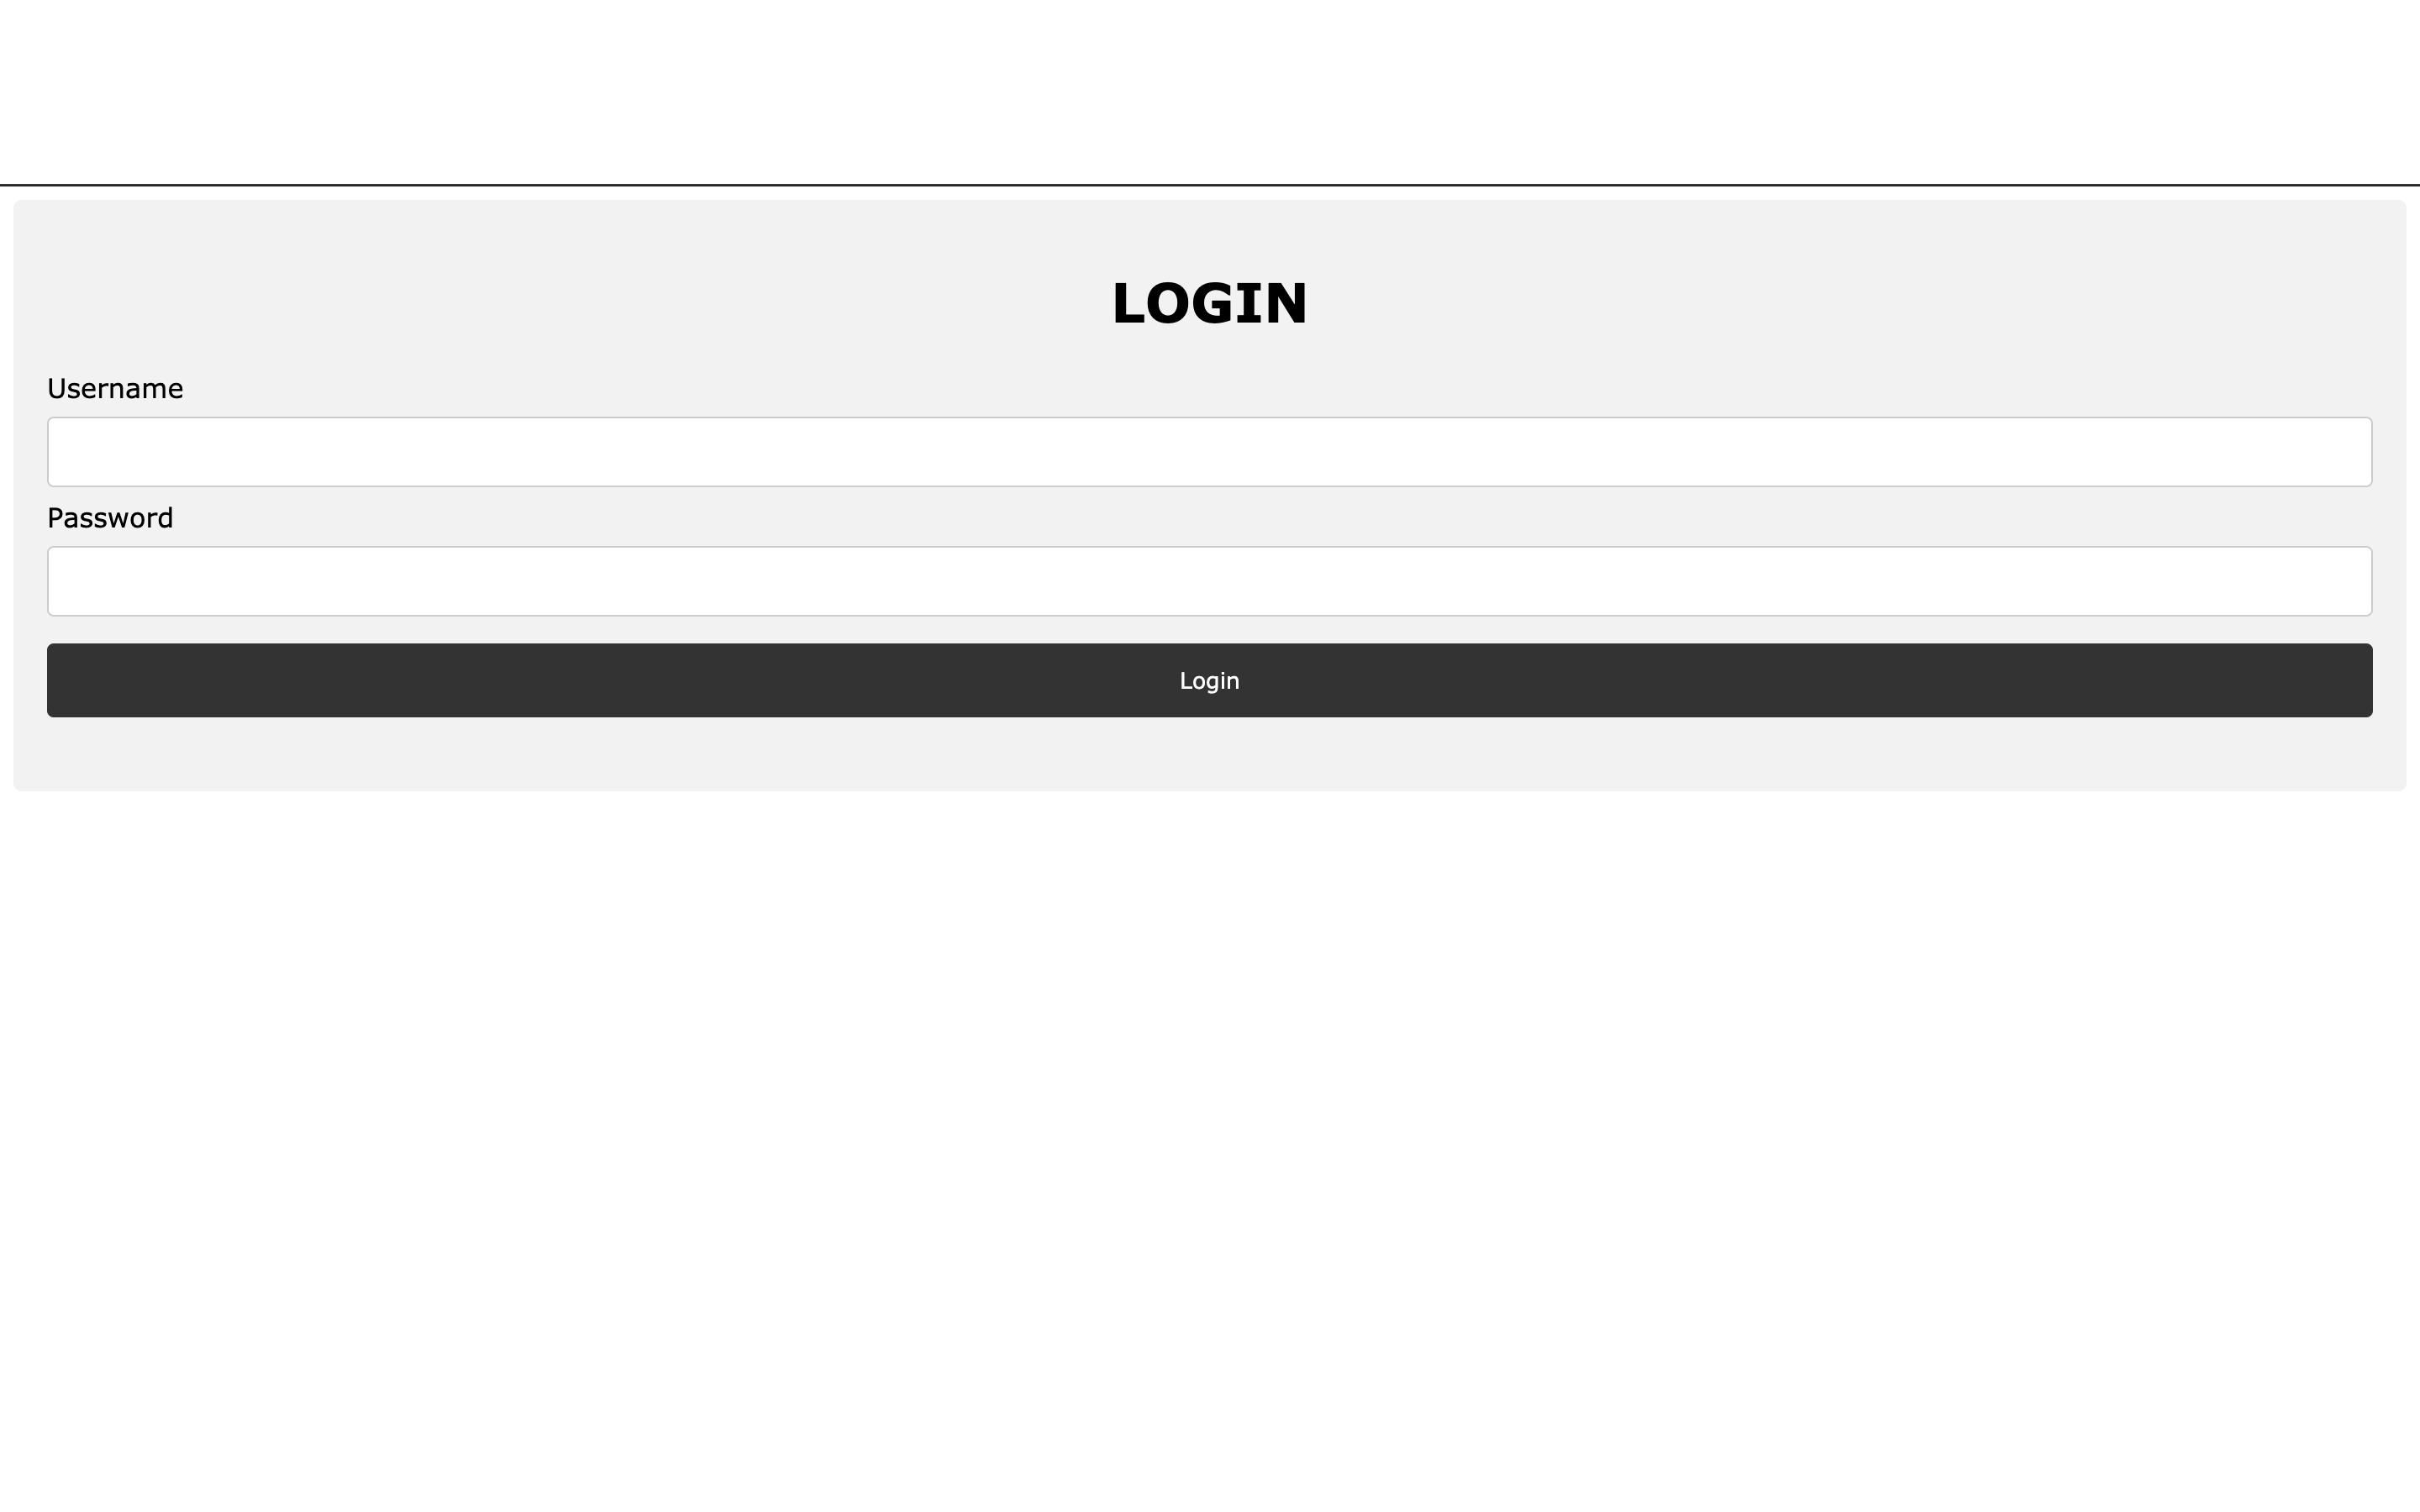
\includegraphics[scale=0.12]{res/images/login.png}
    \caption{Login}
\end{figure}
\subsection{Visualizzazione situazione in real time del magazzino}
\begin{itemize}
    \item Dopo l'autenticazione, tramite il menù selezionare il pulsante "Mappa";
    \item viene visualizzata la planimetria del magazzino con la relativa legenda e la rappresentazione dei muletti che si spostano;
    \item la tabella a destra rappresentano le liste di task con i relativi muletti che le stanno soddisfando.
    
\end{itemize}

\begin{figure}[H]
    \centering
    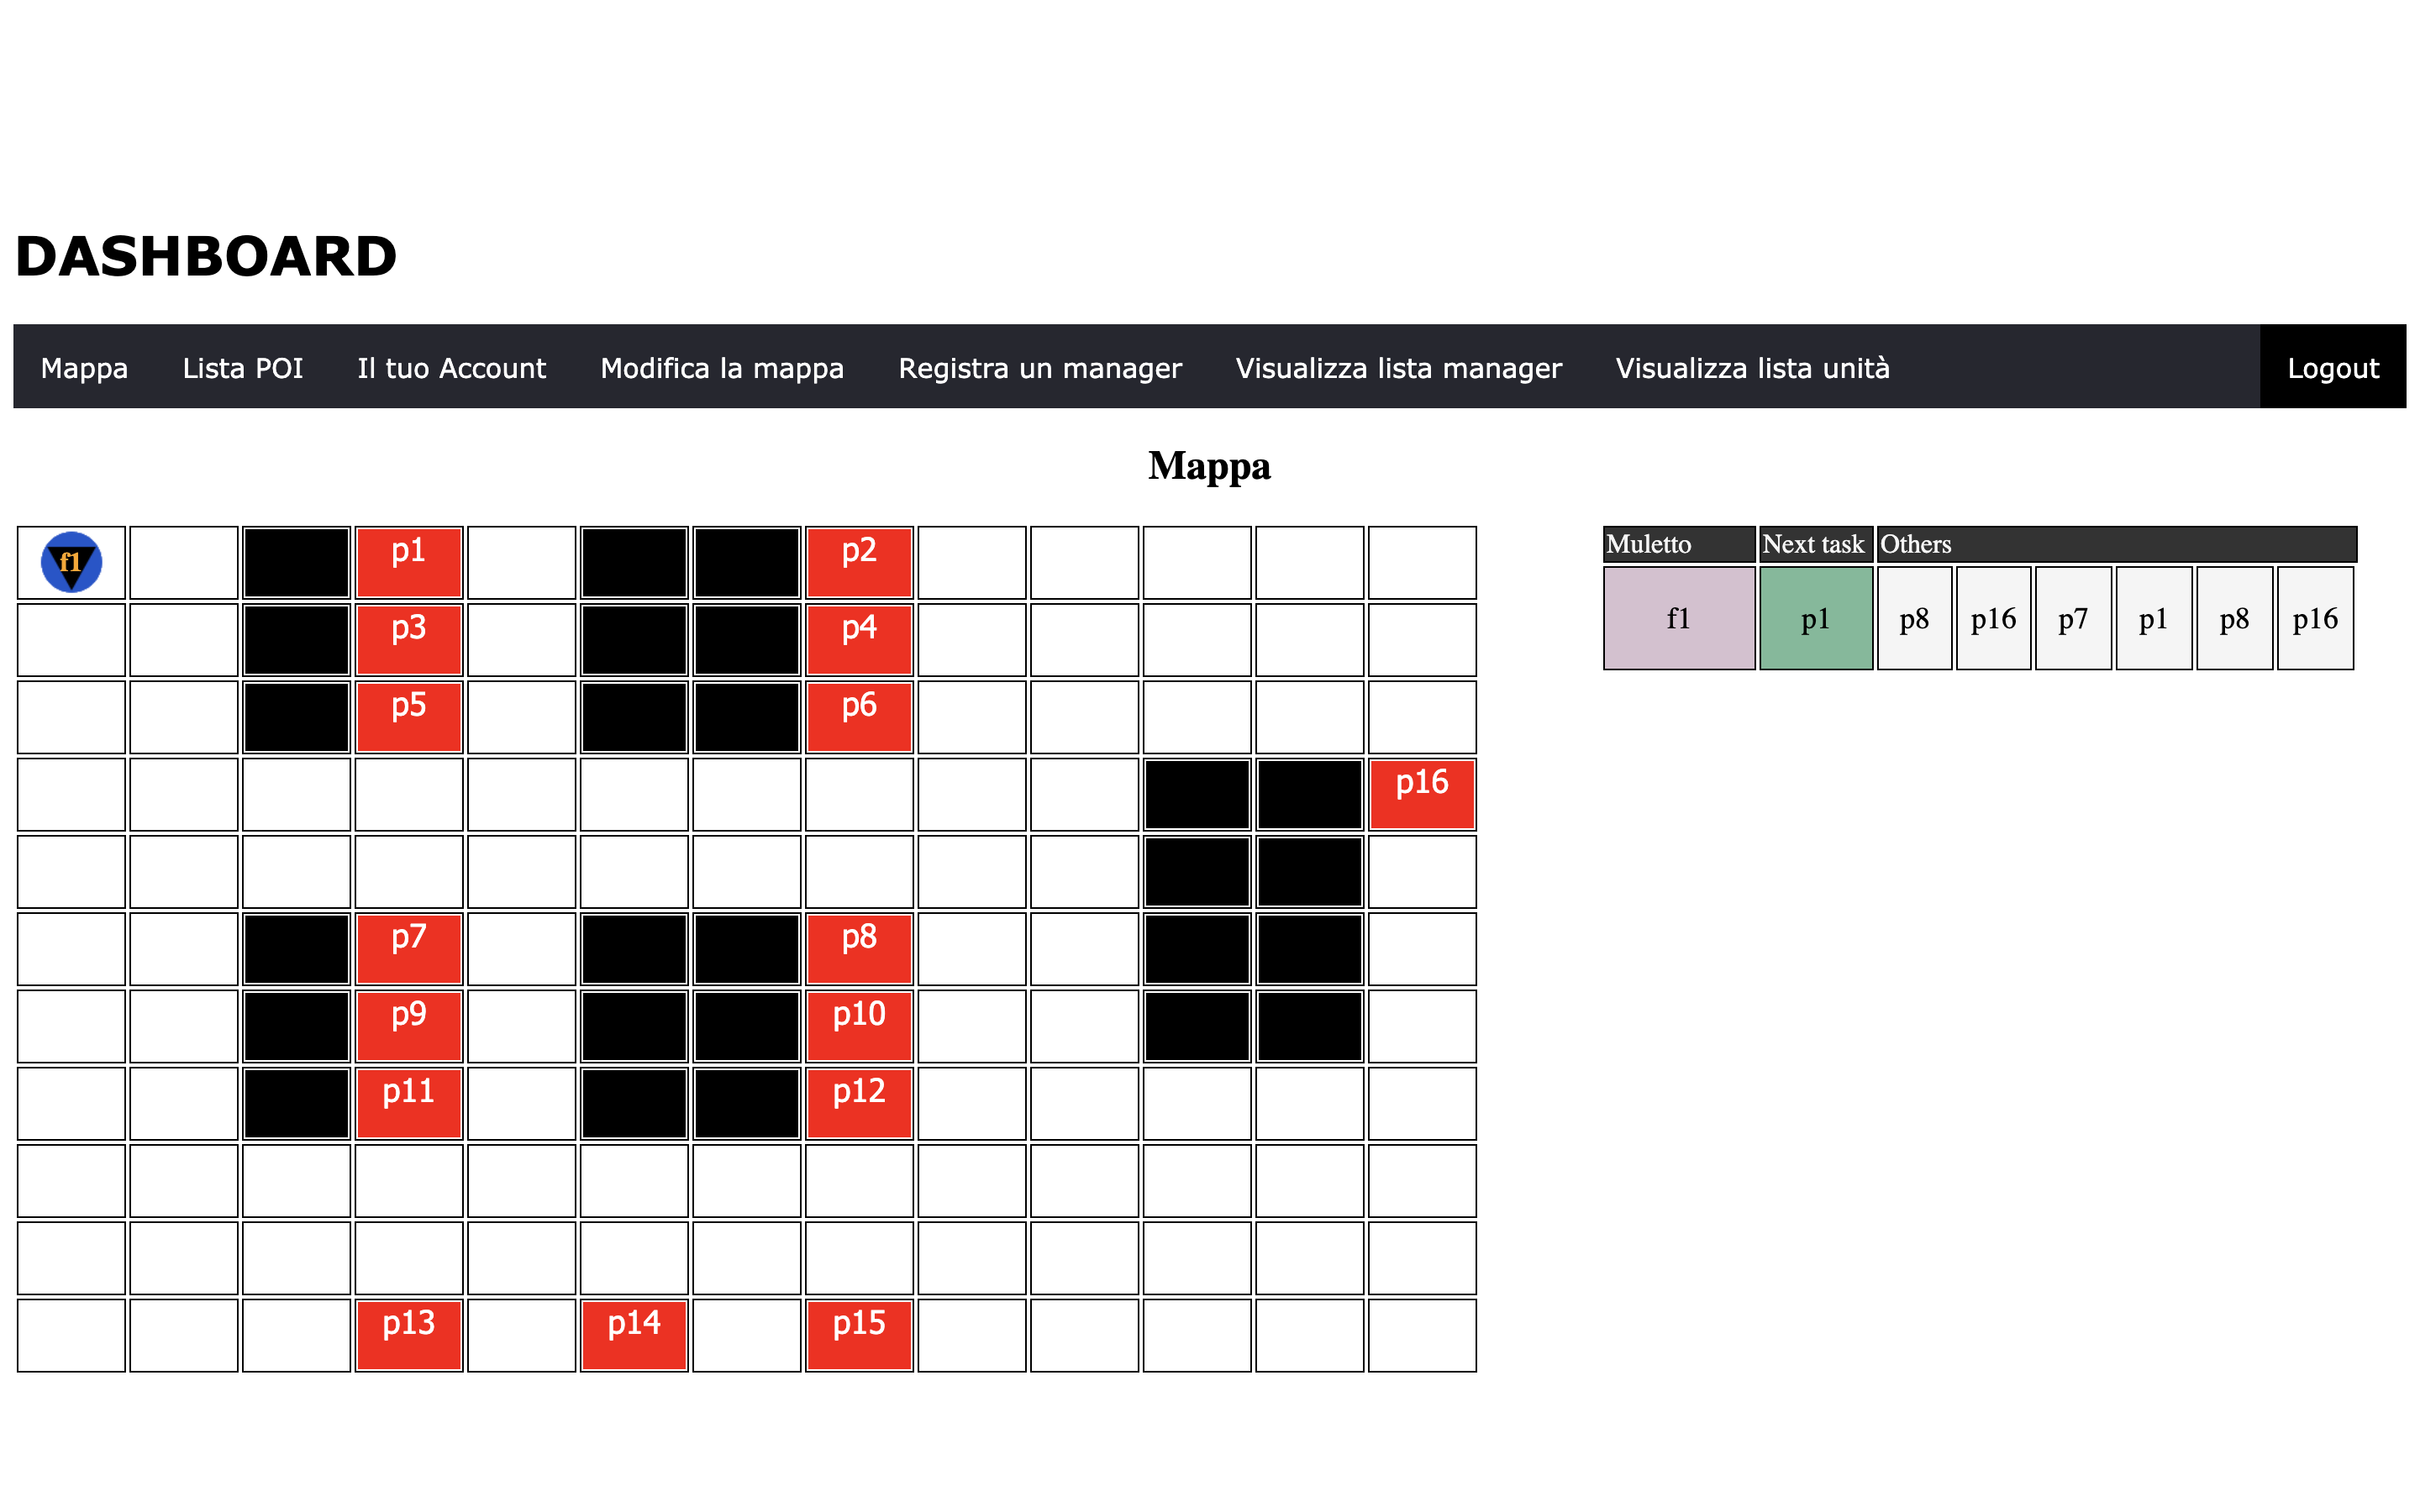
\includegraphics[scale=0.12]{res/images/map_user.png}
    \caption{Schermata visualizzazione in real time del magazzino}
\end{figure}

\subsection{Visualizzazione lista completa punti di interesse}
\begin{itemize}
    \item Dopo l'autenticazione, tramite il menù selezionare il pulsante "Lista POI";
    \item si viene indirizzati alla pagina con l'elenco di tutti i punti di interesse presenti nel magazzino.

\end{itemize}

\begin{figure}[H]
    \centering
    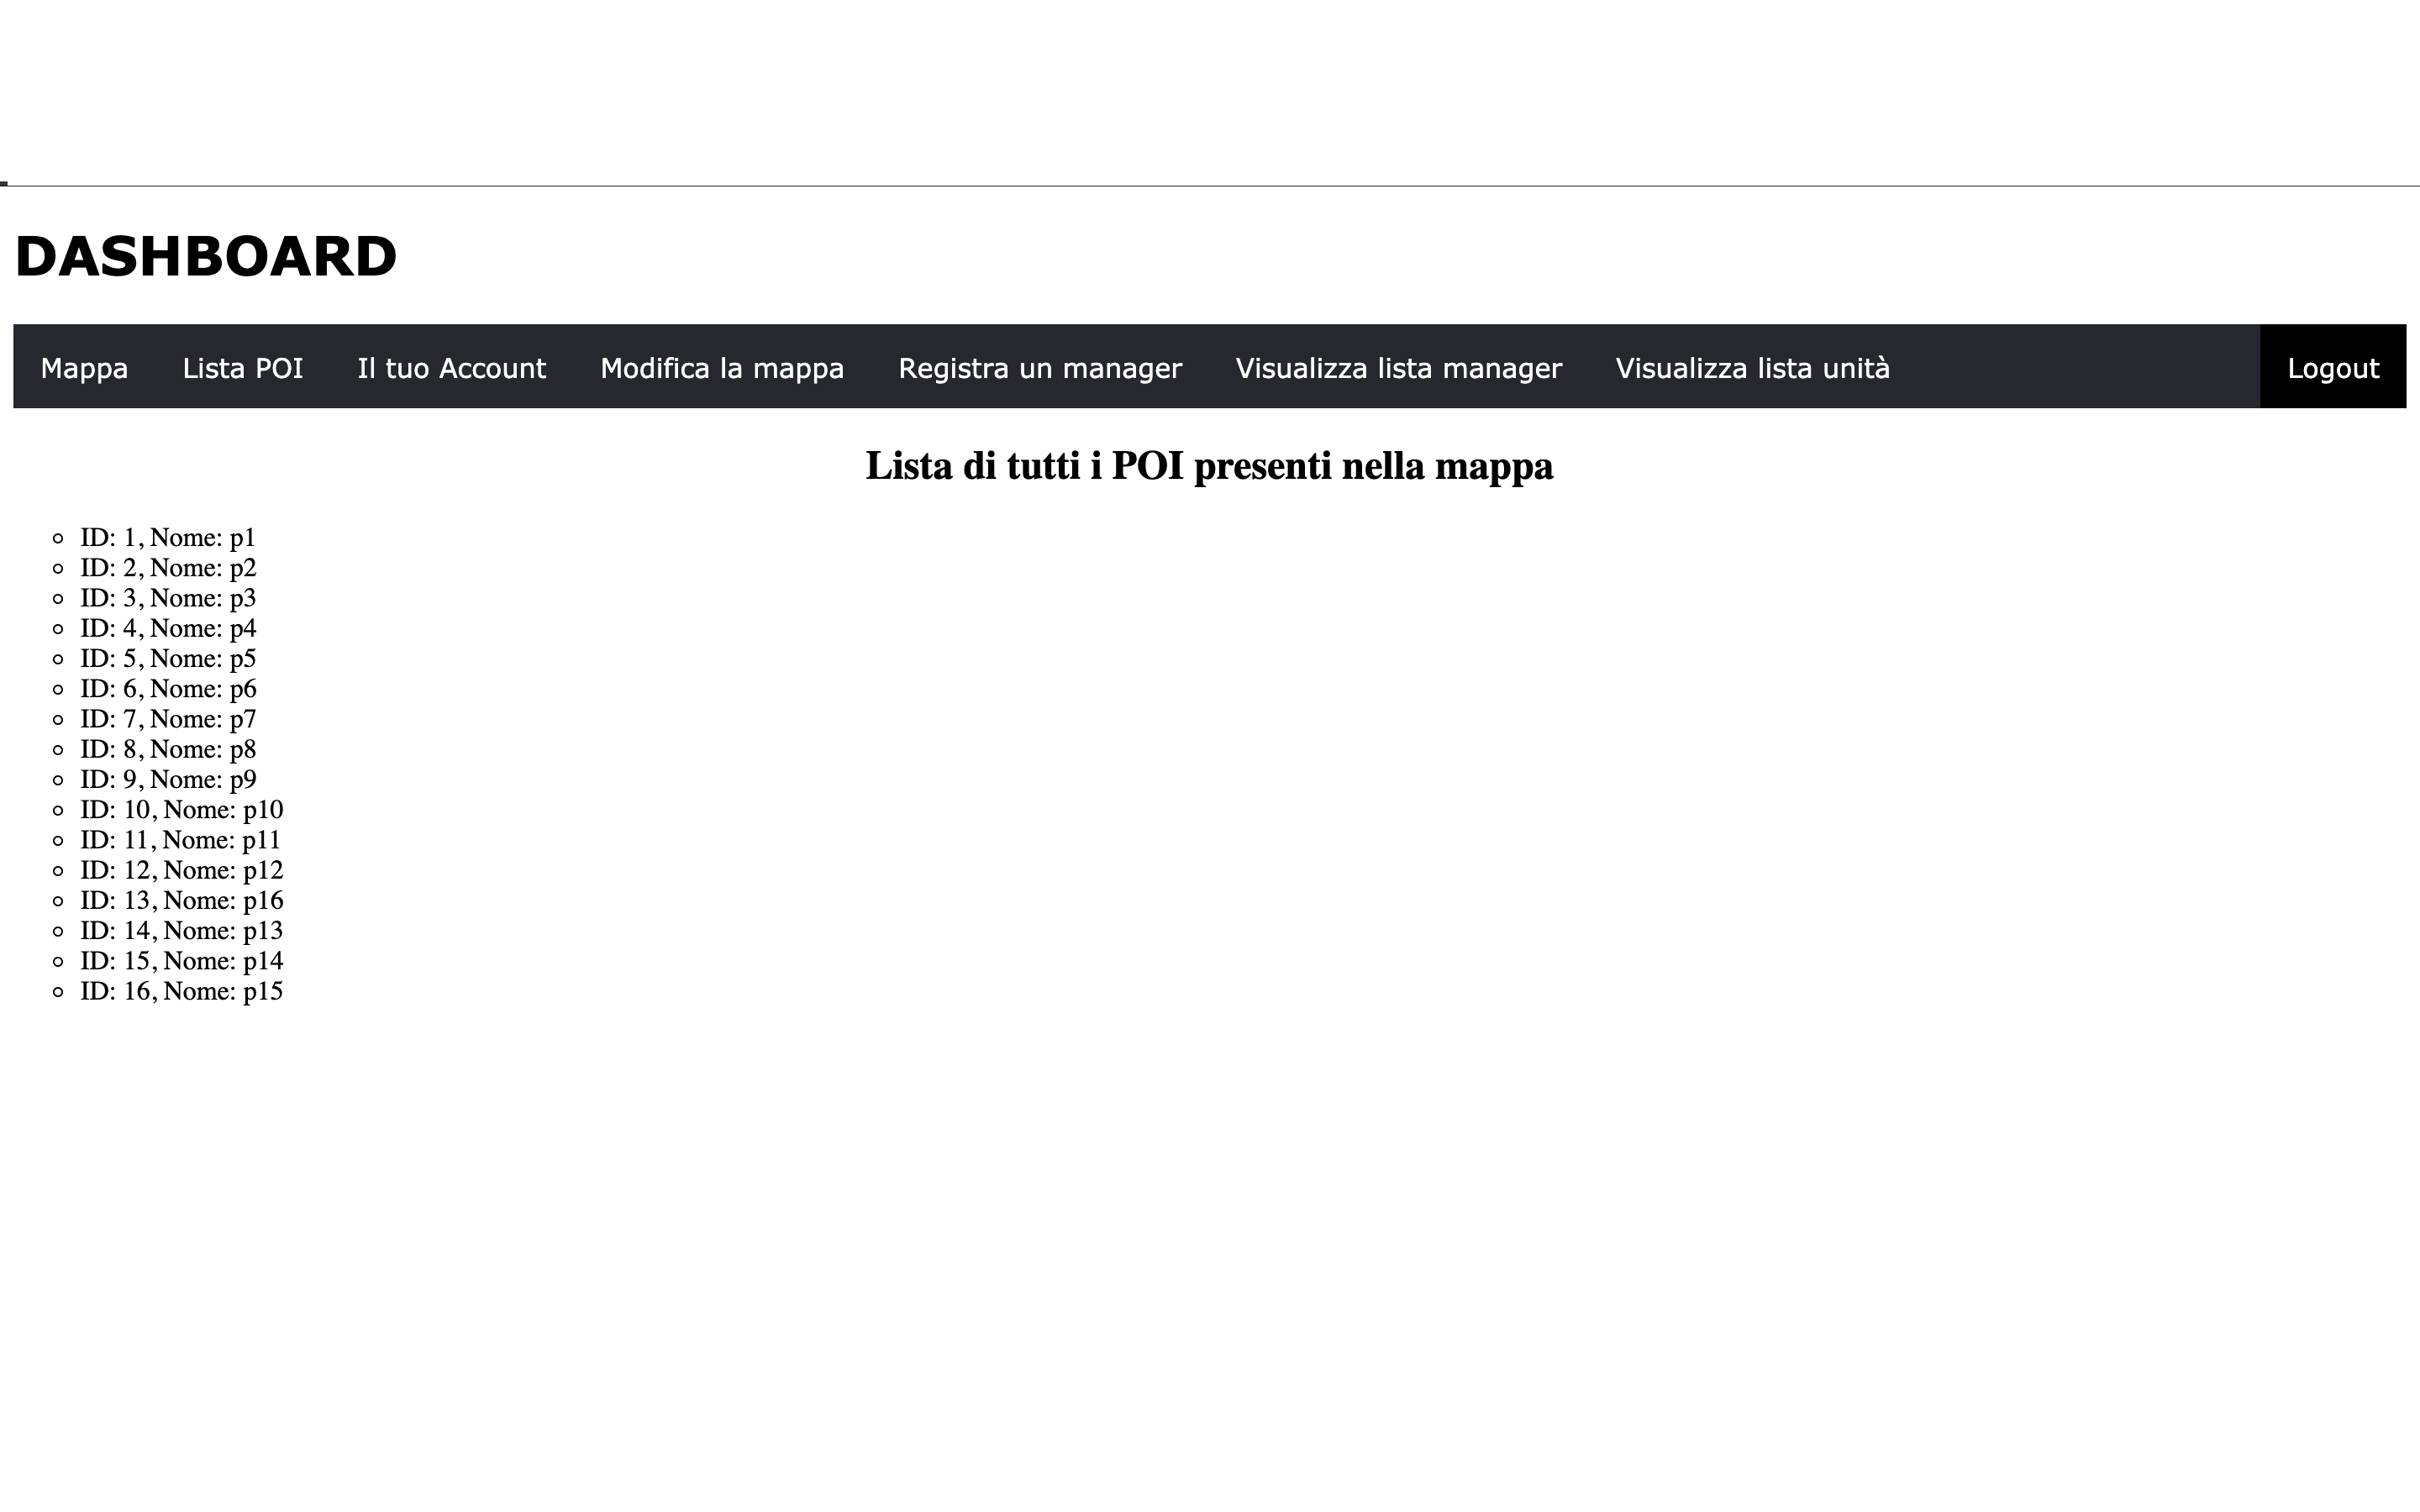
\includegraphics[scale=0.12]{res/images/listpoi_user.png}
    \caption{Schermata guida automatica dell'unità}
\end{figure}

\subsection{Visualizzazione dati del proprio profilo e modifica}
\begin{itemize}
    \item Dopo l'autenticazione, tramite il menù selezionare il pulsante "Il tuo account";
    \item si viene indirizzati alla pagina con i propri dati utente: Name, Surname, Password;
    \item se si desidera modificare alcuni campi, è necessario scrivere nell'apposito form i nuovi dati e premere il pulsante "Salva Modifiche". Se si intende cambiare la Password, l'inserimento nei due campi deve coincidere.
\end{itemize}
\begin{figure}[H]
    \centering
    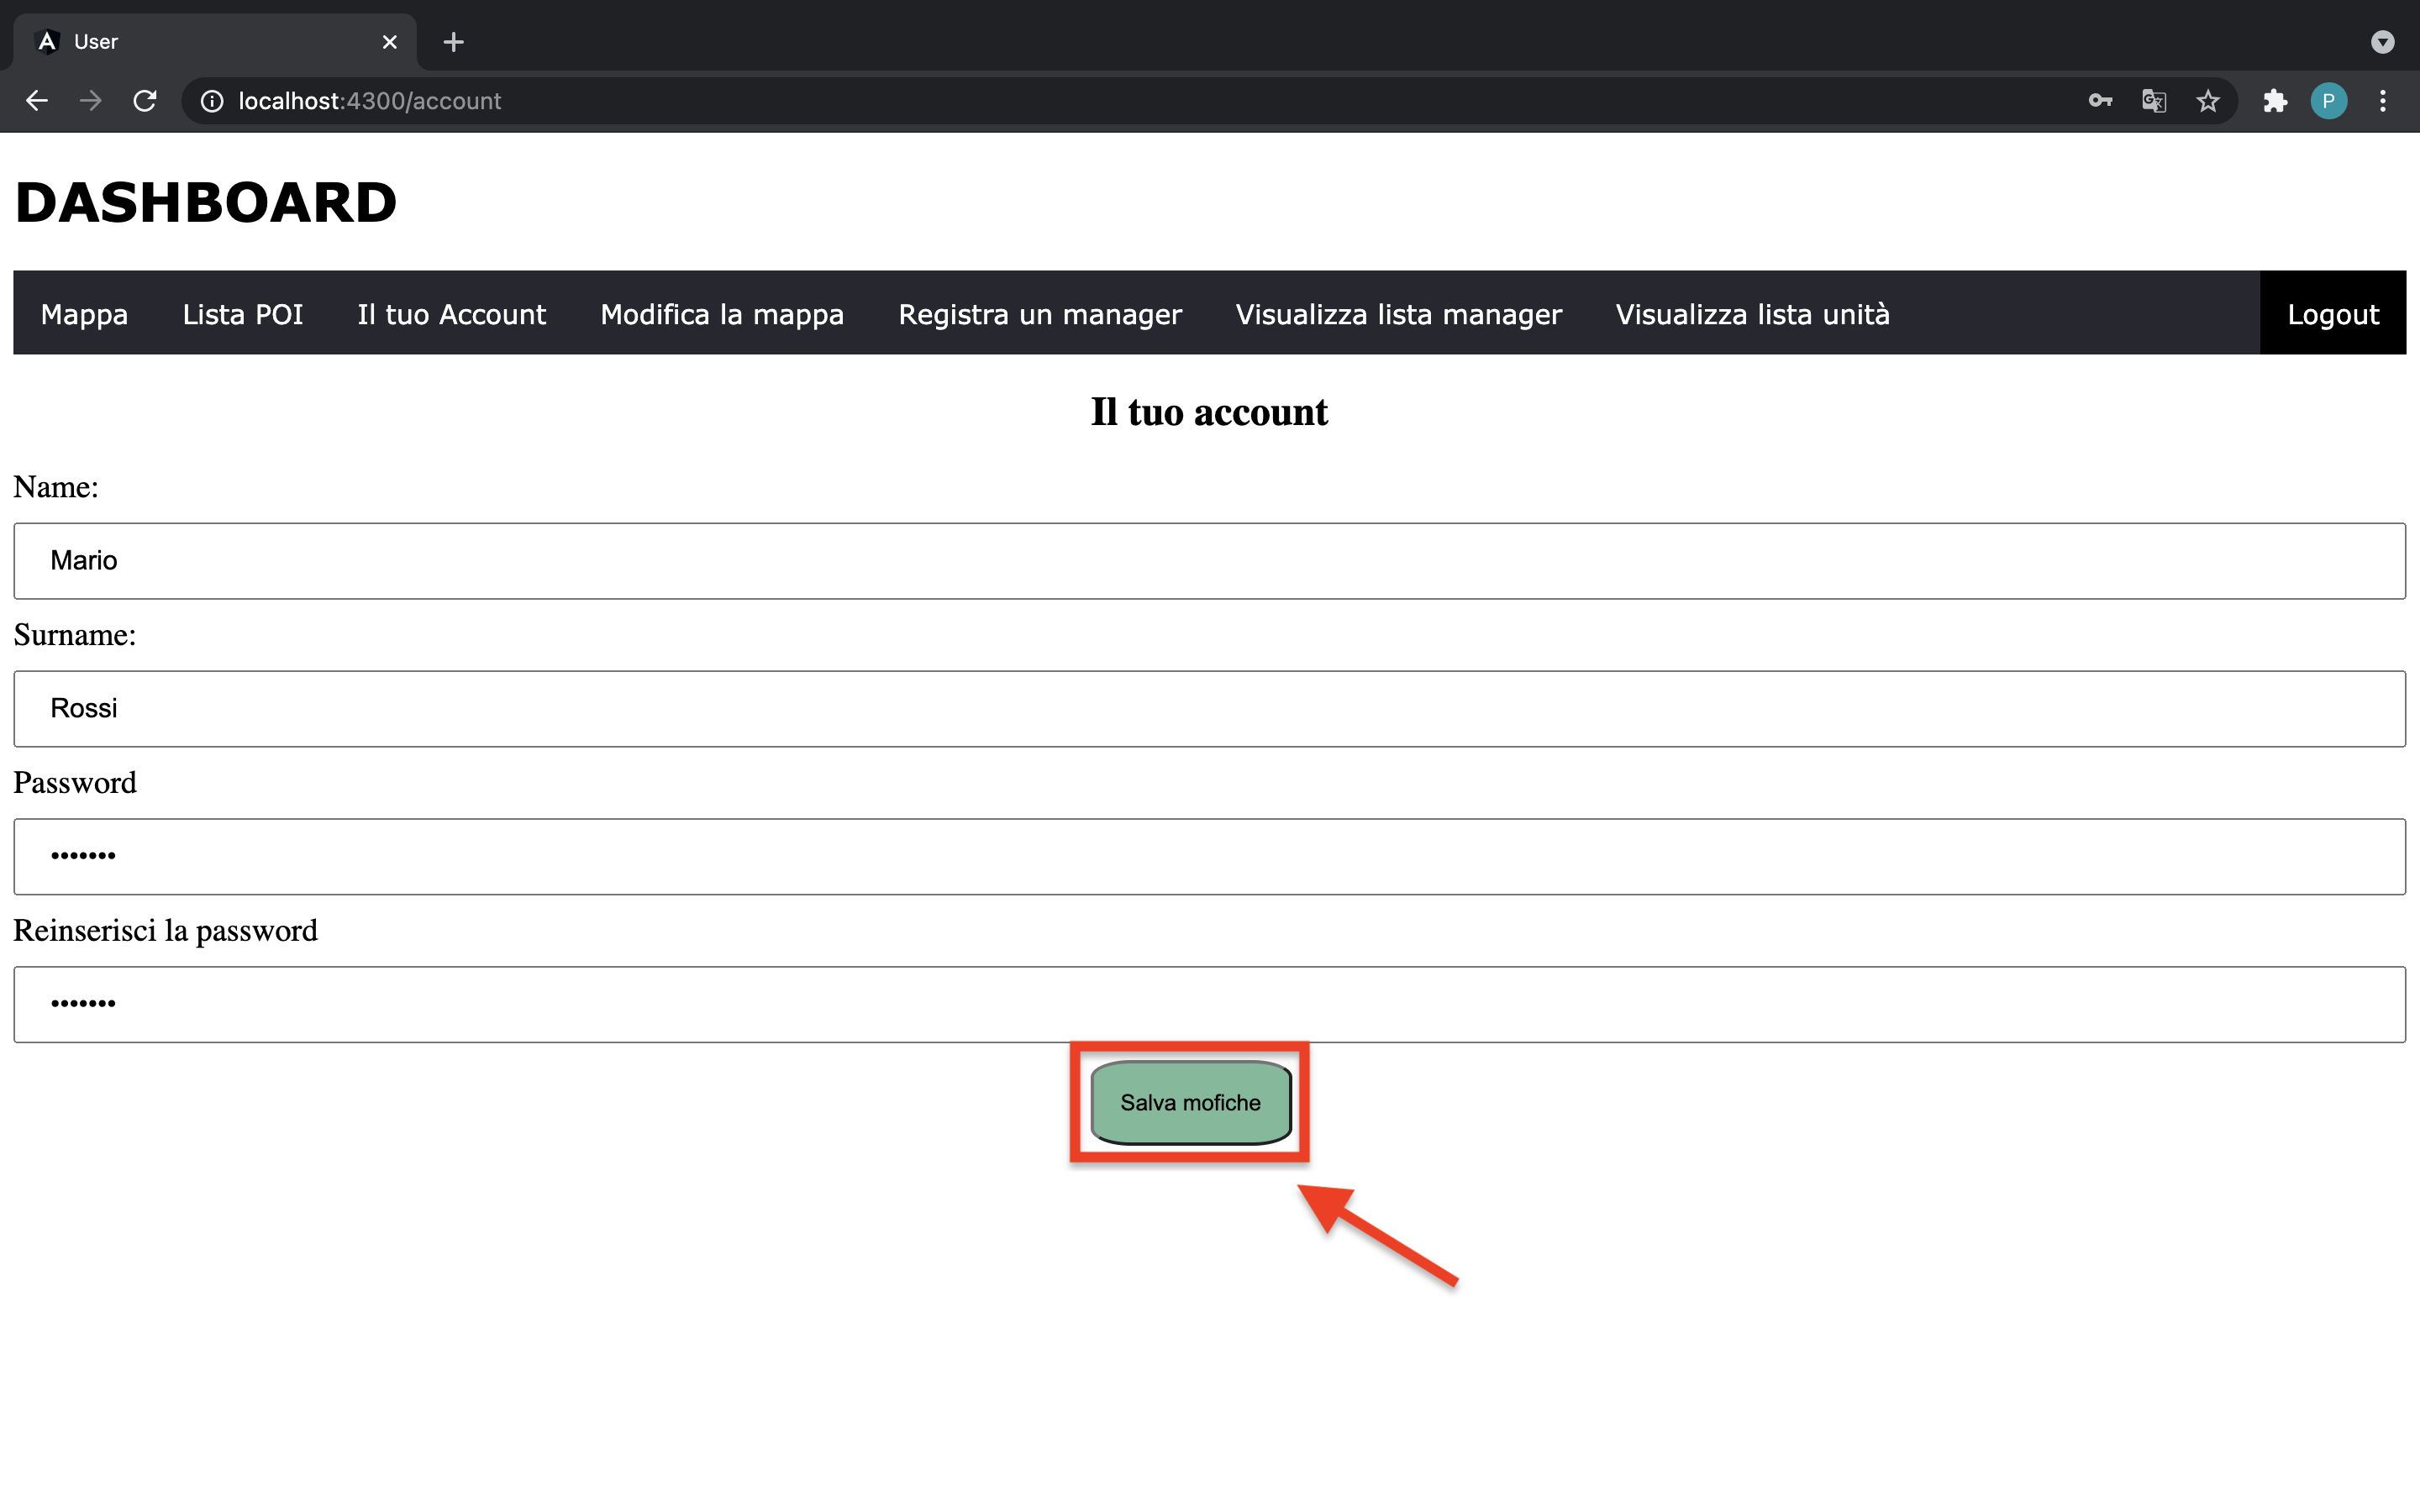
\includegraphics[scale=0.12]{res/images/account_user.png}
    \caption{Schermata proprio profilo}
\end{figure}

\subsection{Registrazione di un nuovo utente}
\begin{itemize}
    \item Dopo l'autenticazione, tramite il menù selezionare il pulsante "Registra un manager";
    \item si viene indirizzati alla pagina con i campi da compilare: Nome, Cognome;
\end{itemize}
\begin{figure}[H]
    \centering
    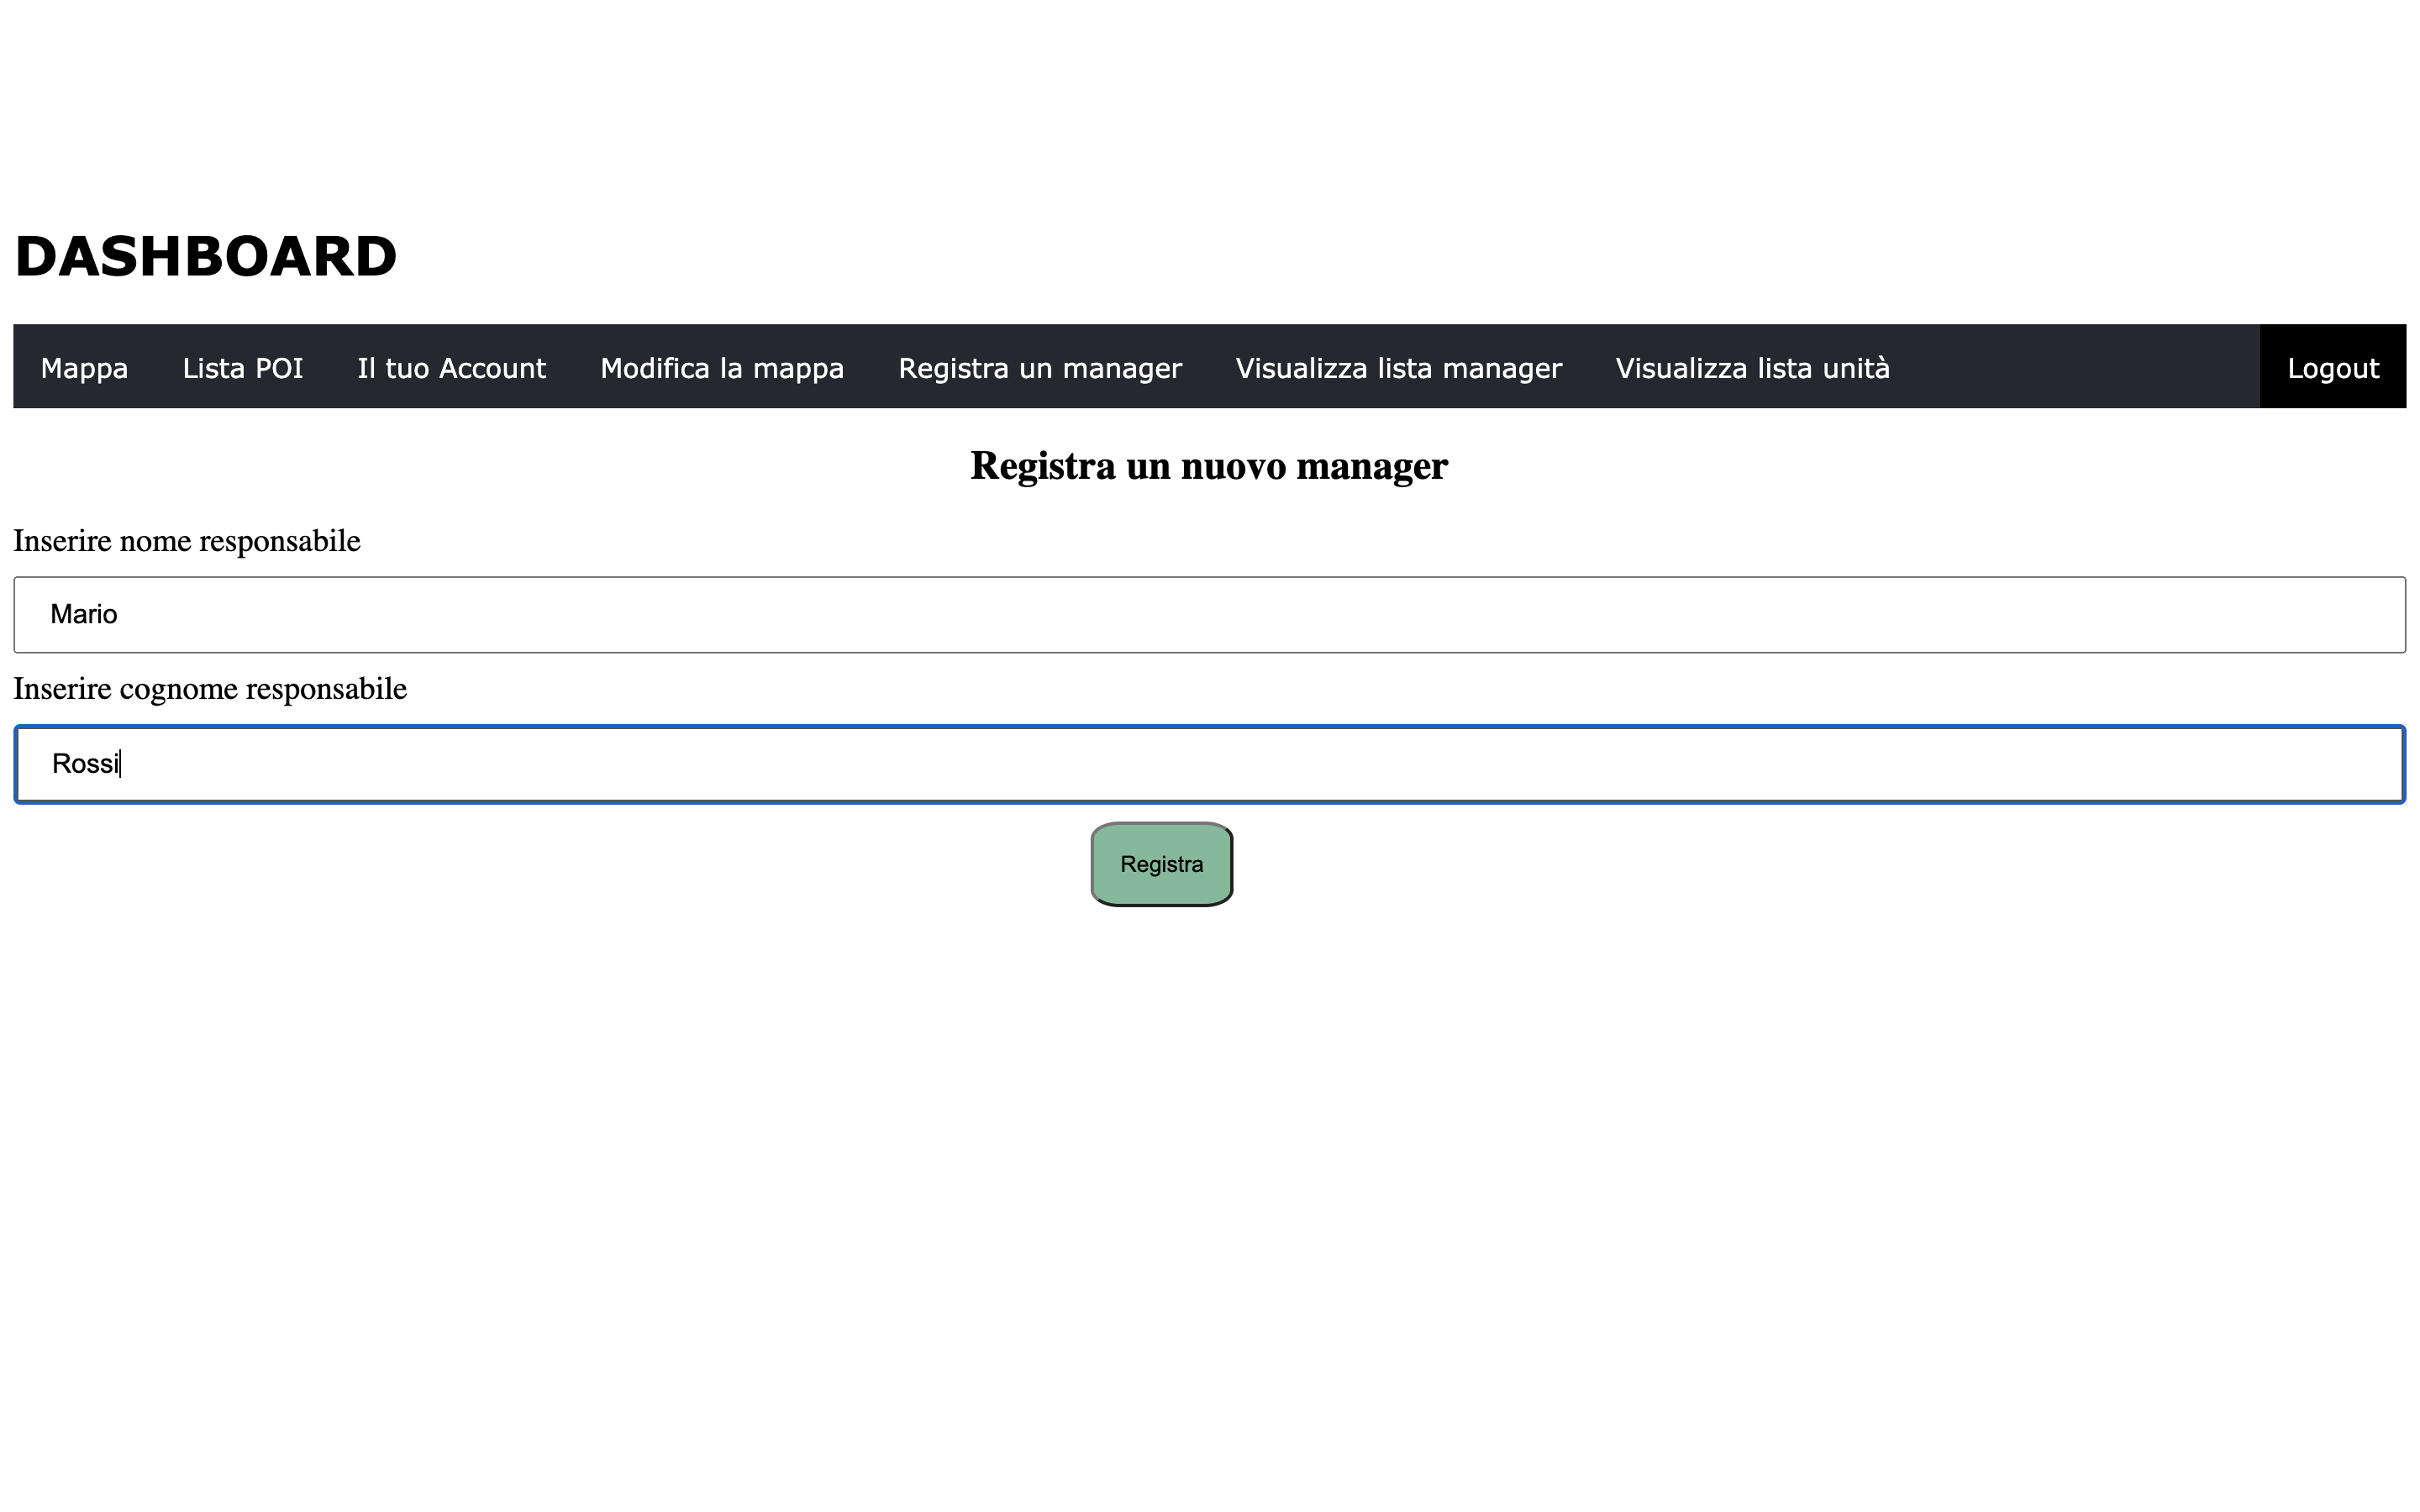
\includegraphics[scale=0.12]{res/images/newmanager_admin.png}
    \caption{Schermata registrazione manager 1}
\end{figure}
\begin{itemize}
    \item inserire i dati e premere sul pulsante "Conferma";
    \item viene visualizzato a video la password e il codice identificativo da riferire al nuovo utente per il suo primo accesso.
\end{itemize}


\begin{figure}[H]
    \centering
    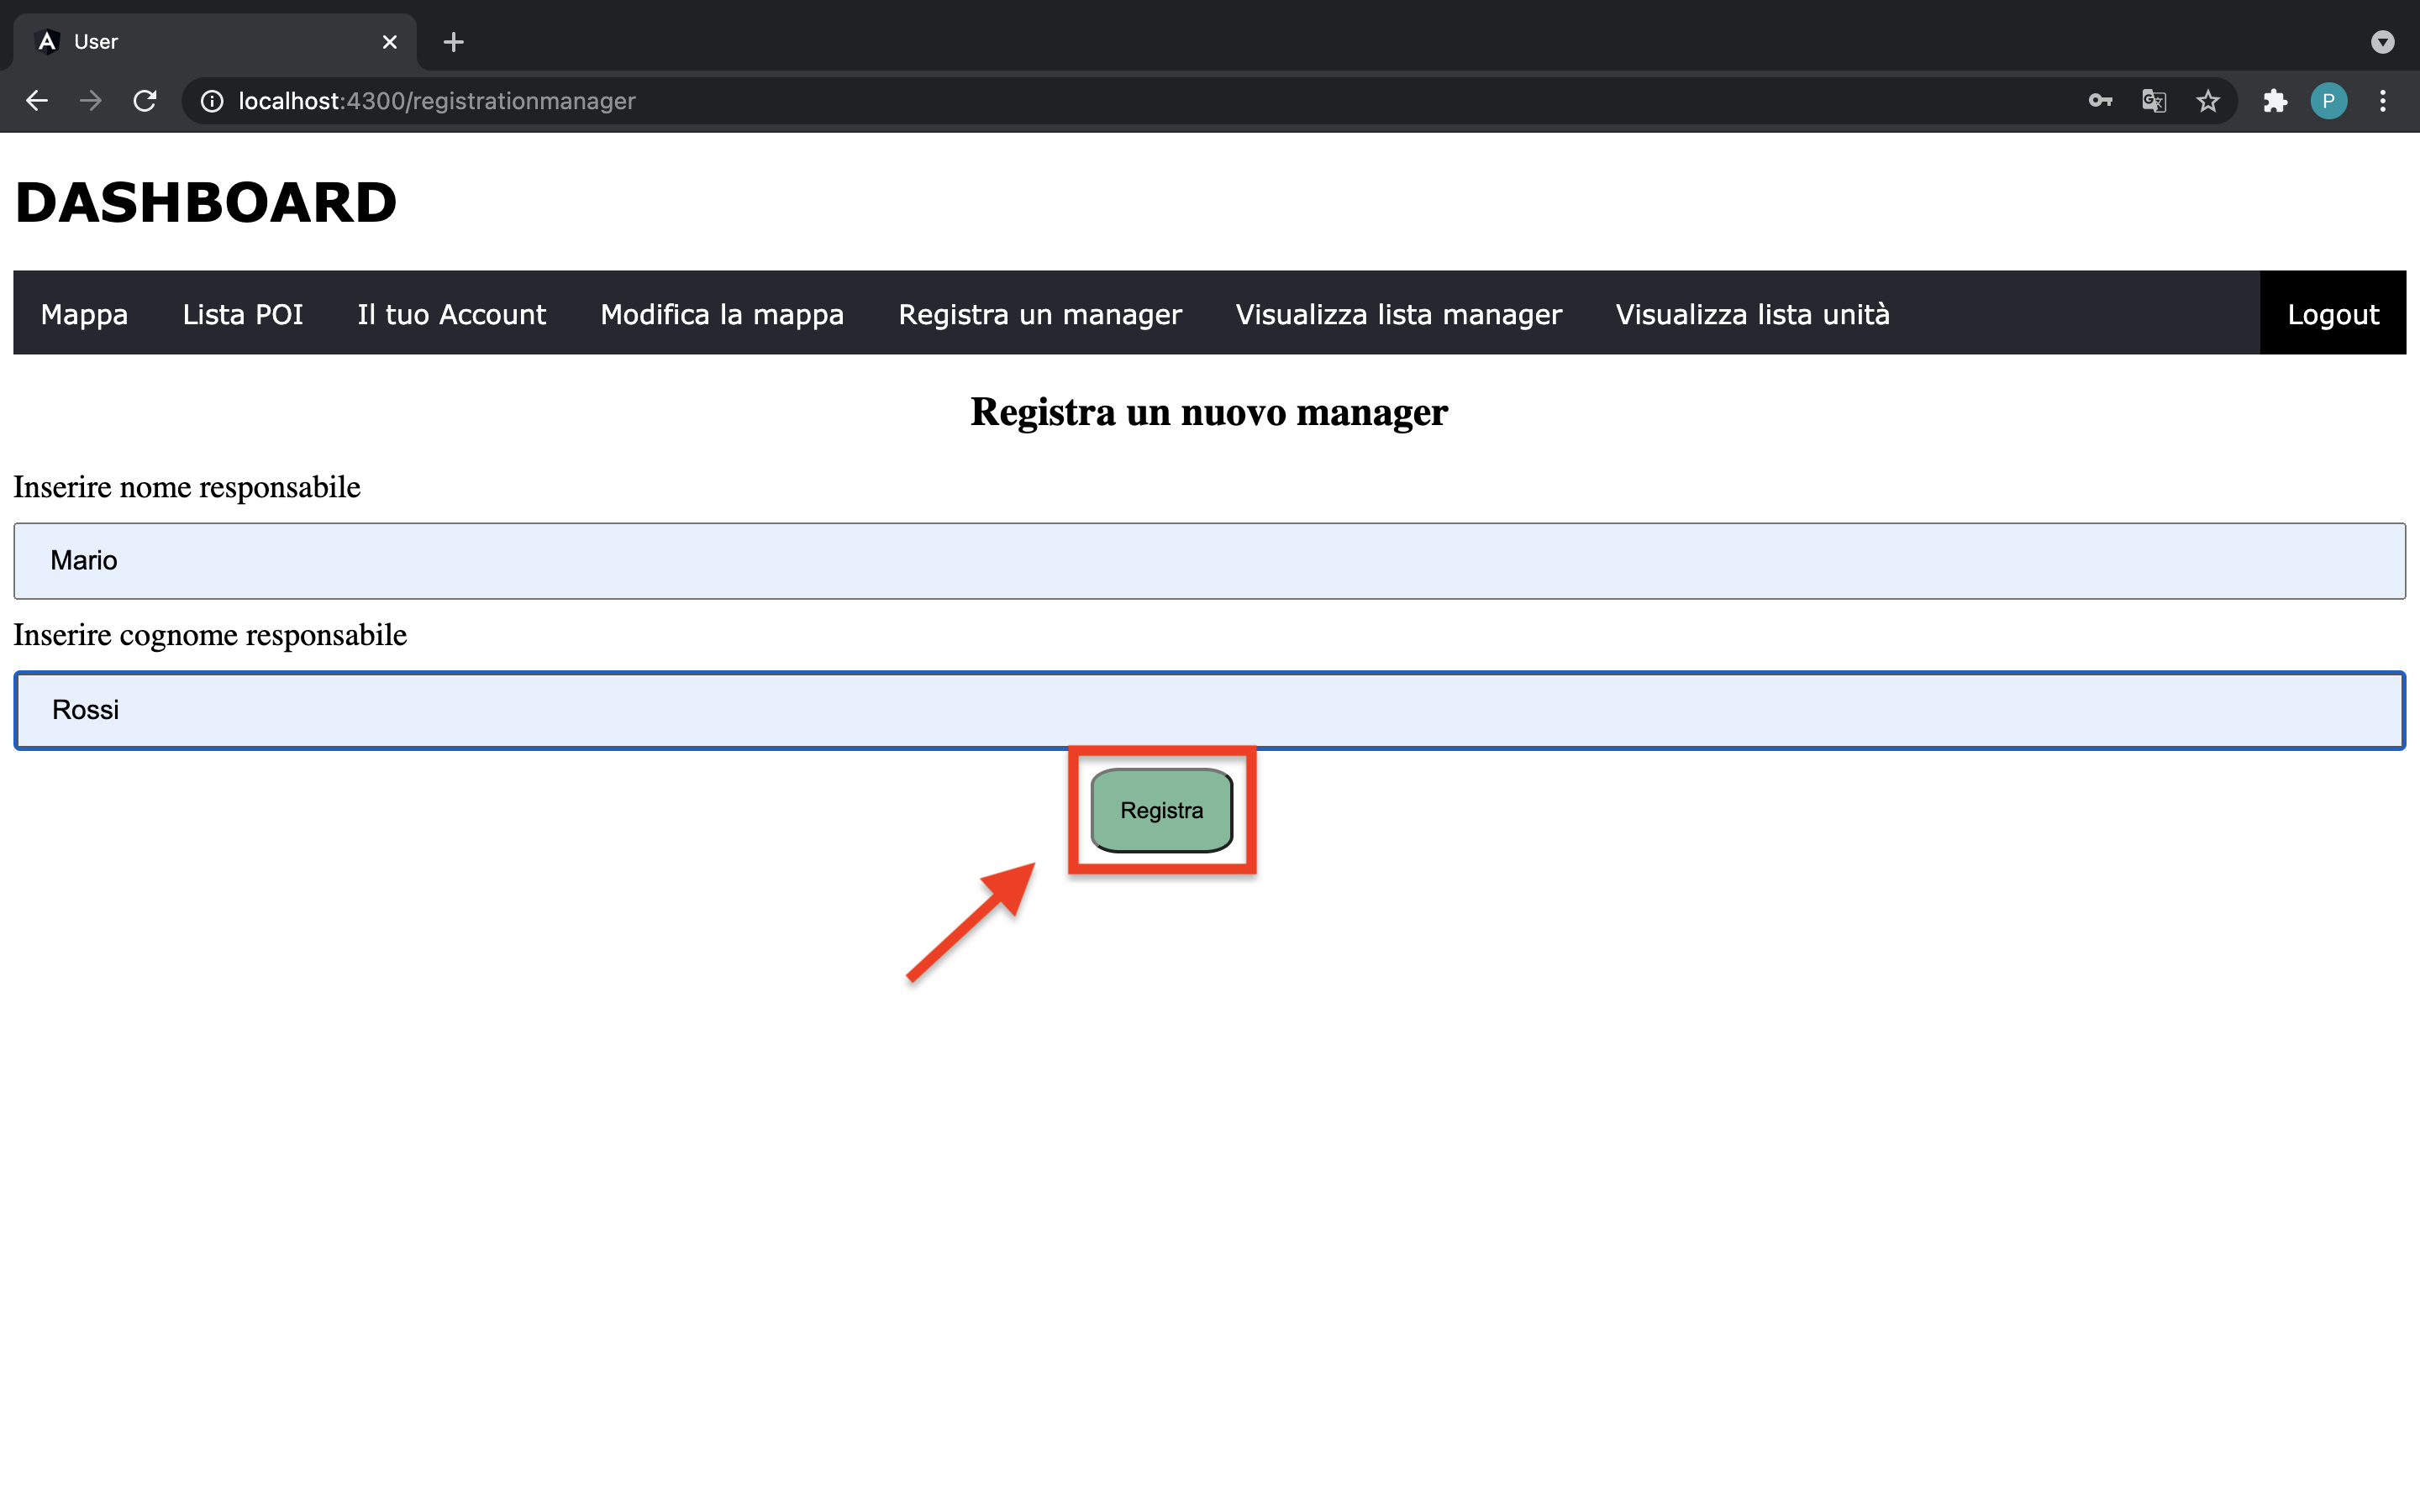
\includegraphics[scale=0.12]{res/images/newmanager_2.png}
    \caption{Schermata registrazione manager 2}
\end{figure}

\subsection{Gestione account già presenti}
\begin{itemize}
    \item Dopo l'autenticazione, tramite il menù selezionare il pulsante "Visualizza lista manager";
    \item si viene indirizzati alla pagina con la lista di tutti gli account presenti;
    \item per ogni account è possibile:
        \begin{itemize}
            \item cambiare i campi "Name" e "Surname" e premere su "Conferma Modifica" per confermare le modifiche;
            \item premere il pulsate "Elimina" per cancellare definitivamente un account dal sistema;
            \item premere il pulsante "Reset password" per cambiare la password di un utente in caso di smarrimento; verrà visualizzata a video la nuova password.
        \end{itemize}
\end{itemize}

\begin{figure}[H]
    \centering
    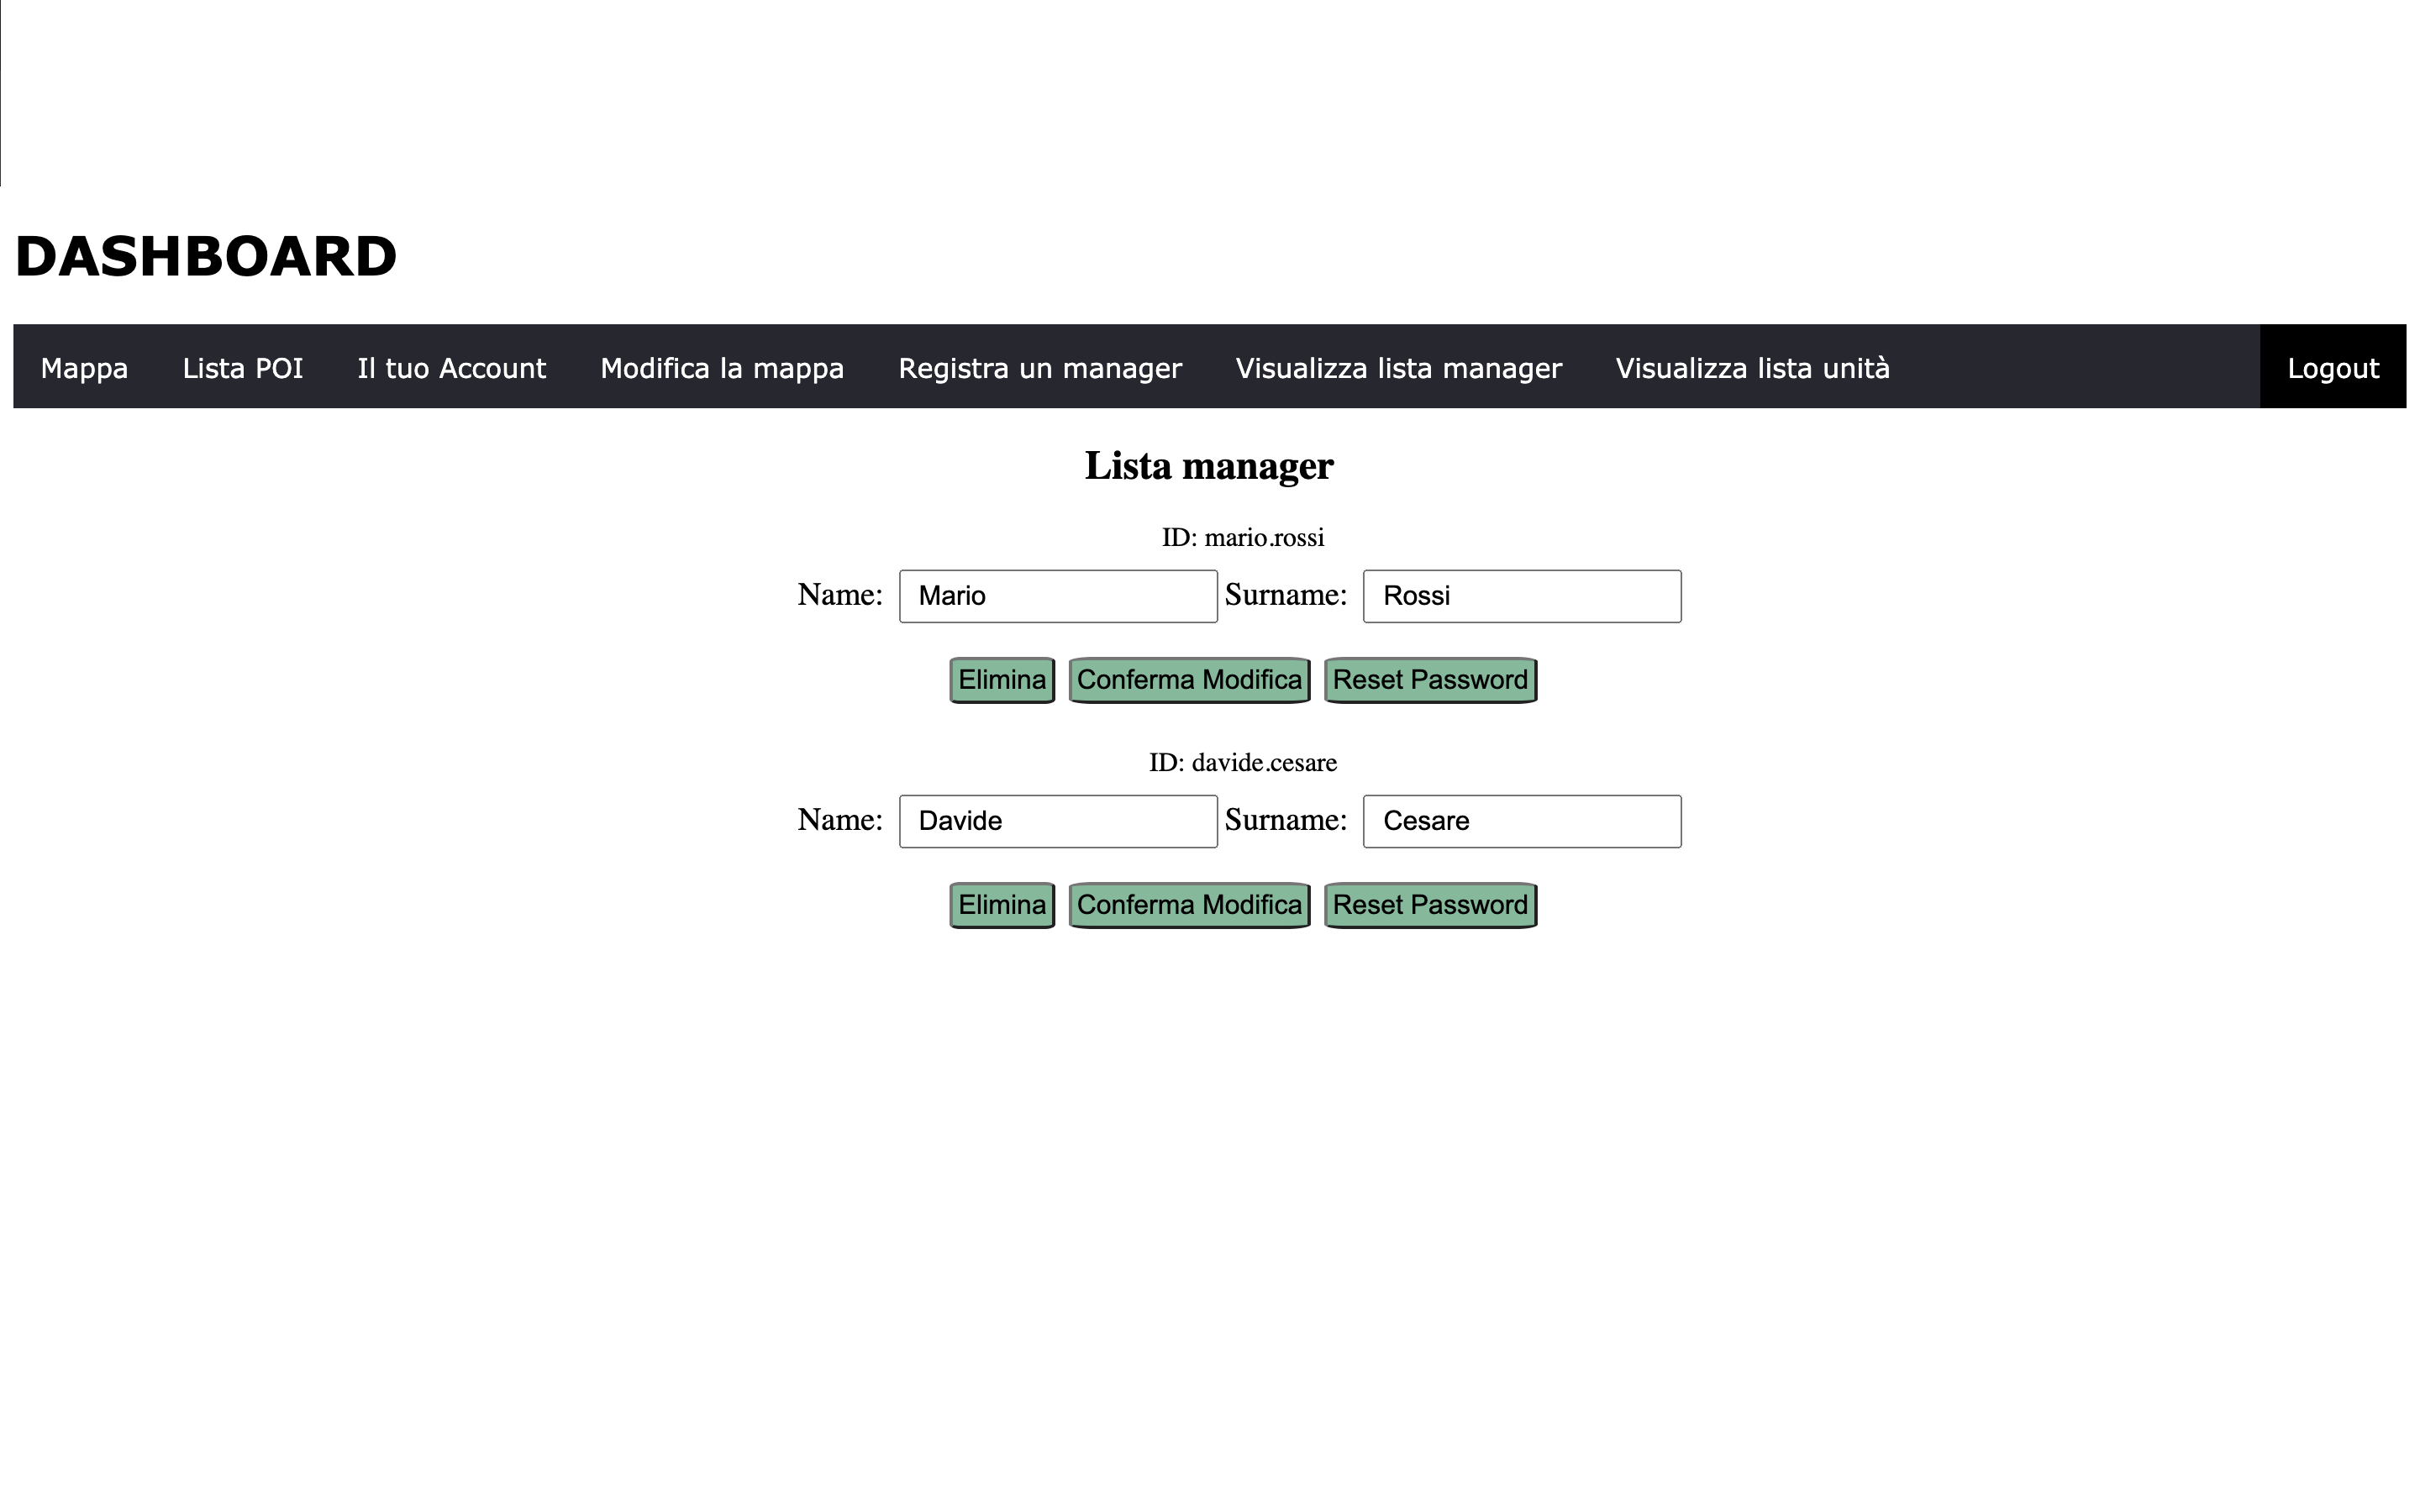
\includegraphics[scale=0.12]{res/images/listmanager_admin.png}
    \caption{Schermata visualizzazione lista di manager}
\end{figure}

\subsection{Modifica mappa del magazzino}
\begin{itemize}
    \item Dopo l'autenticazione, tramite il menù selezionare il pulsante "Modifica mappa";
    \item si viene indirizzati alla pagina con la rappresentazione della mappa;
    \item è possibile intraprendere le seguenti operazioni:
        \begin{itemize}
            \item aggiungere una riga: \\premere sul pulsante "Aggiungi riga" per ampliare la planimetria di una riga;
            \item eliminare una riga: \\premere sul pulsante "Rimuovi riga" per diminuire la planimetria di una riga;
            \item aggiungere una colonna: \\premere sul pulsante "Aggiungi colonna" per ampliare la planimetria di una colonna;
            \item eliminare una colonna: \\premere sul pulsante "Rimuovi colonna" per diminuire la planimetria di una colonna;
            \begin{figure}[H]
                \centering
                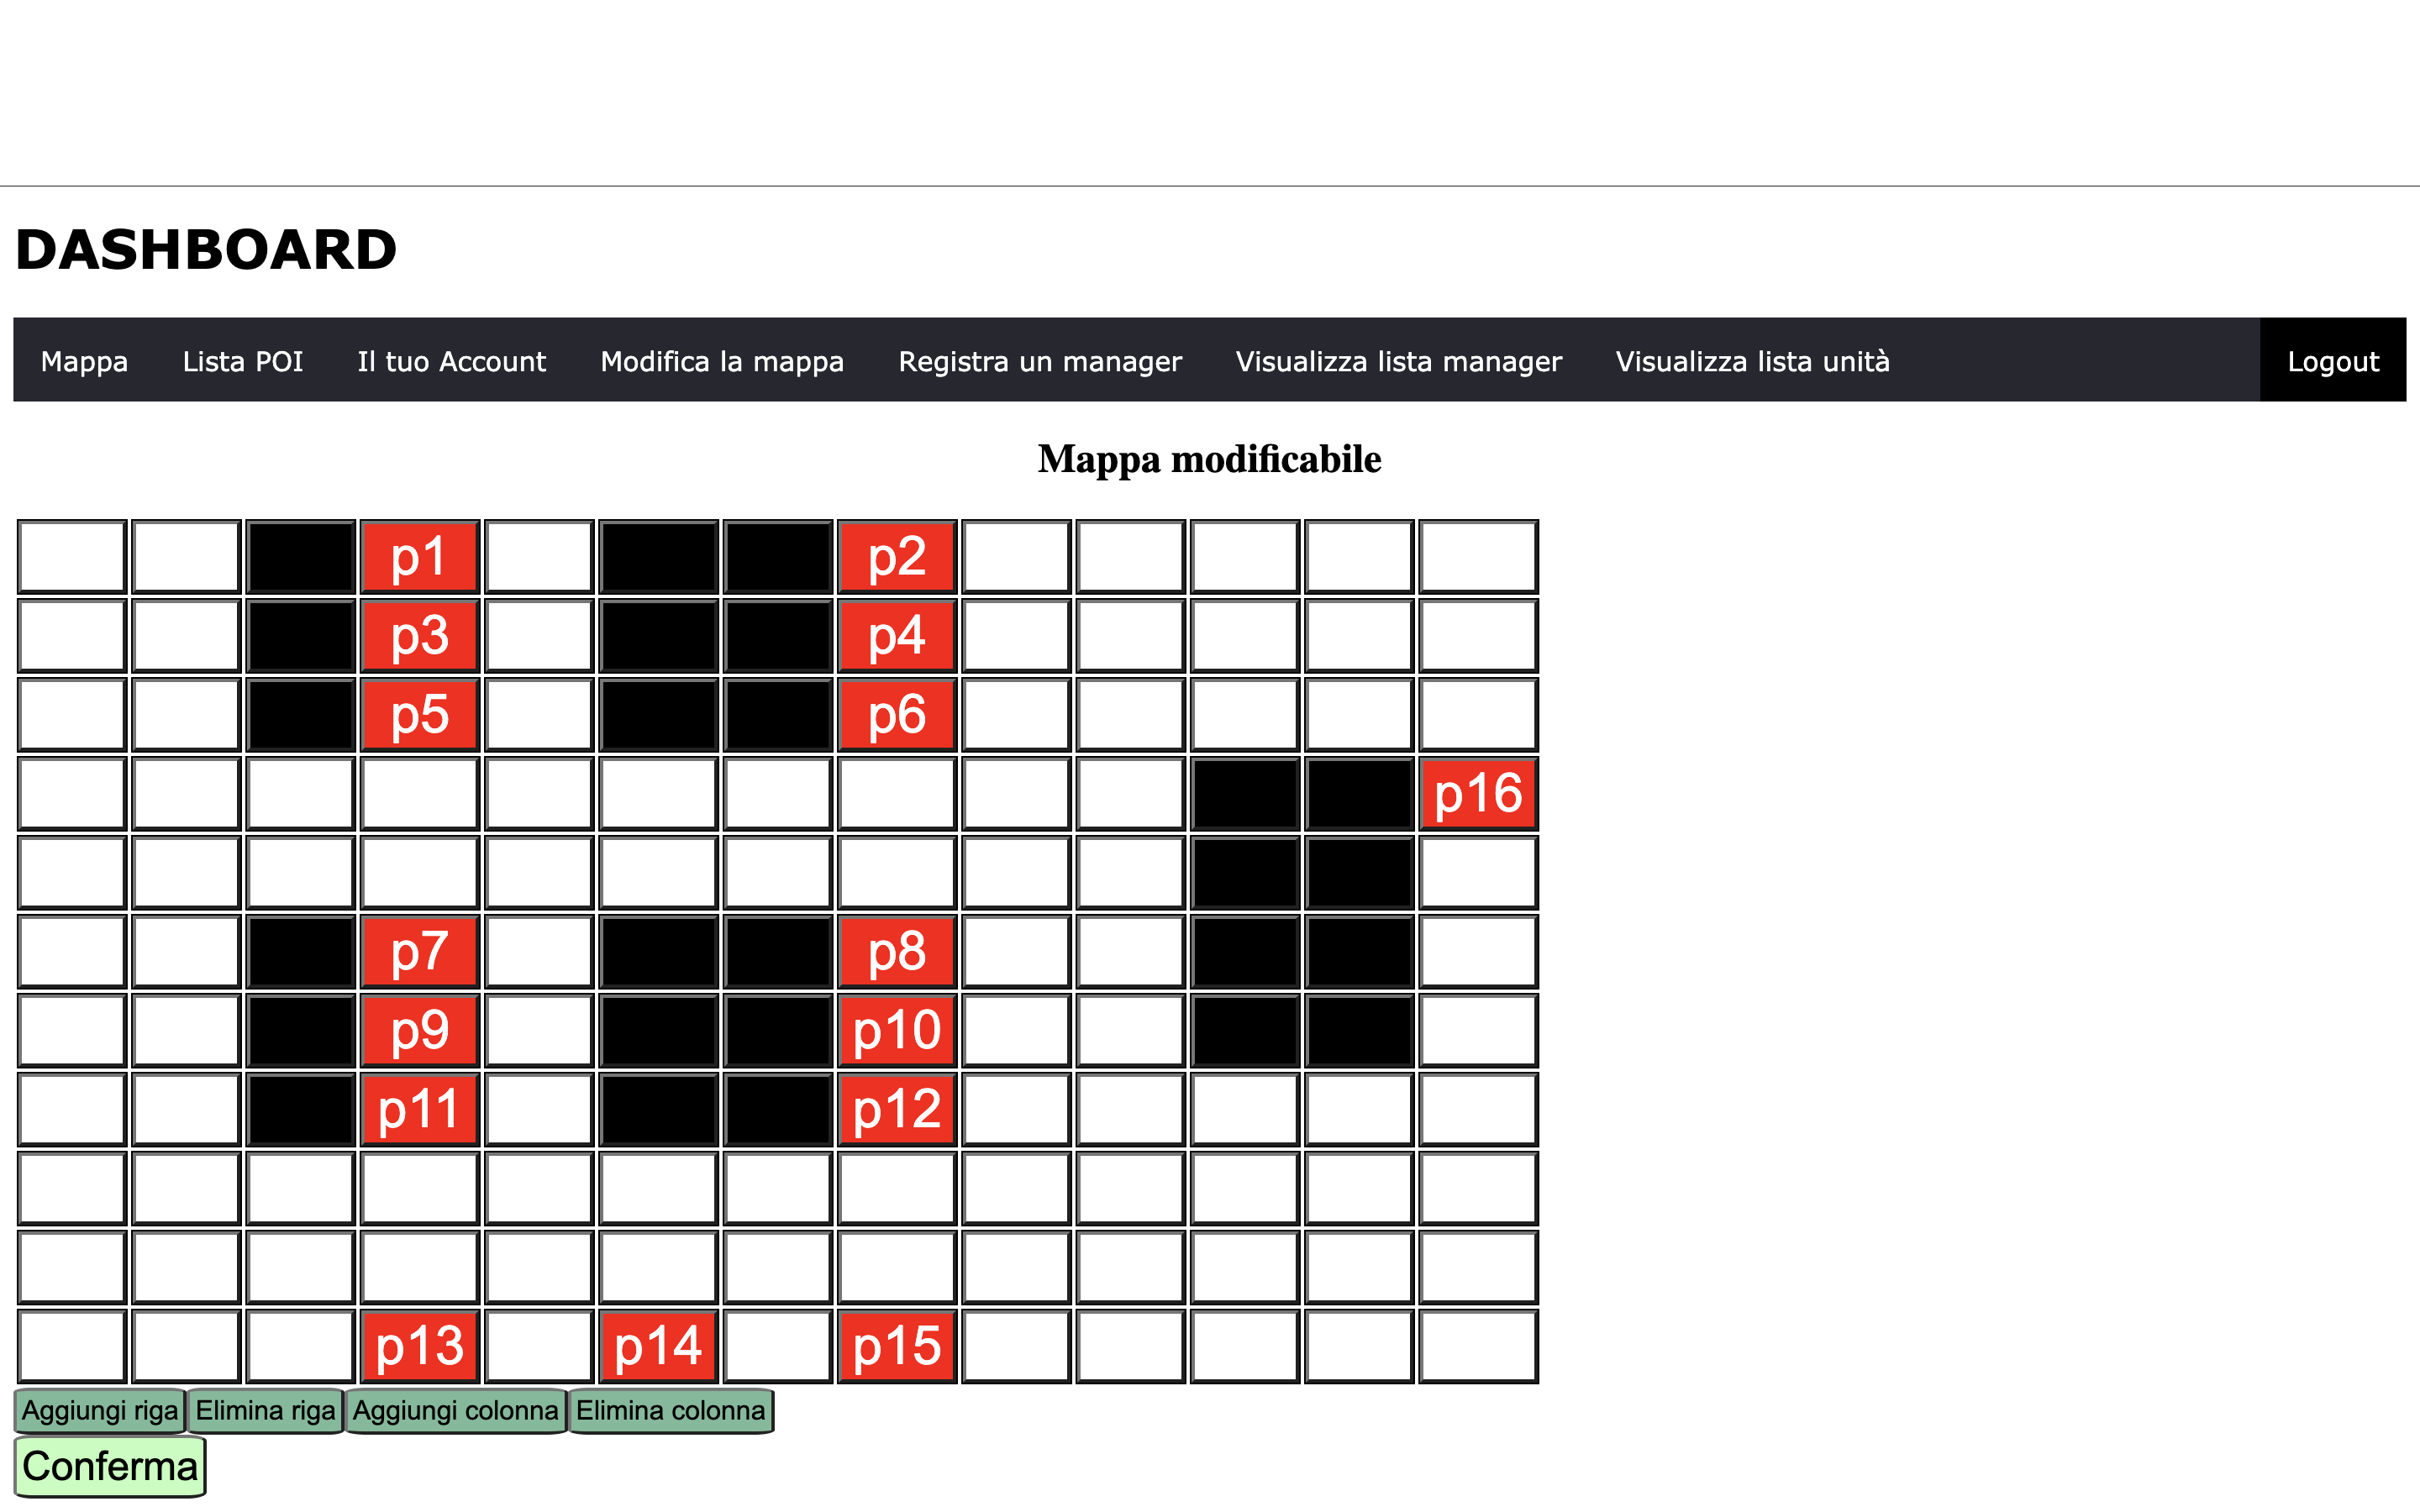
\includegraphics[scale=0.12]{res/images/managemap_admni1.png}
                \caption{Schermata modifica mappa}
            \end{figure}
            \item cambiare il tipo di cella: \\premere sulla cella nella mappa che si intende modificare. Verrà allora visualizzata un'interfaccia con i colori possibili (bianco: zona transitabile, nero: zona non transitabile, frecce: sensi unici, rosso: POI). Nel caso di POI è possibile scrivere l'identificativo. \\Una volta scelto premere sul tasto "Conferma".
        \end{itemize}
        \begin{figure}[H]
            \centering
            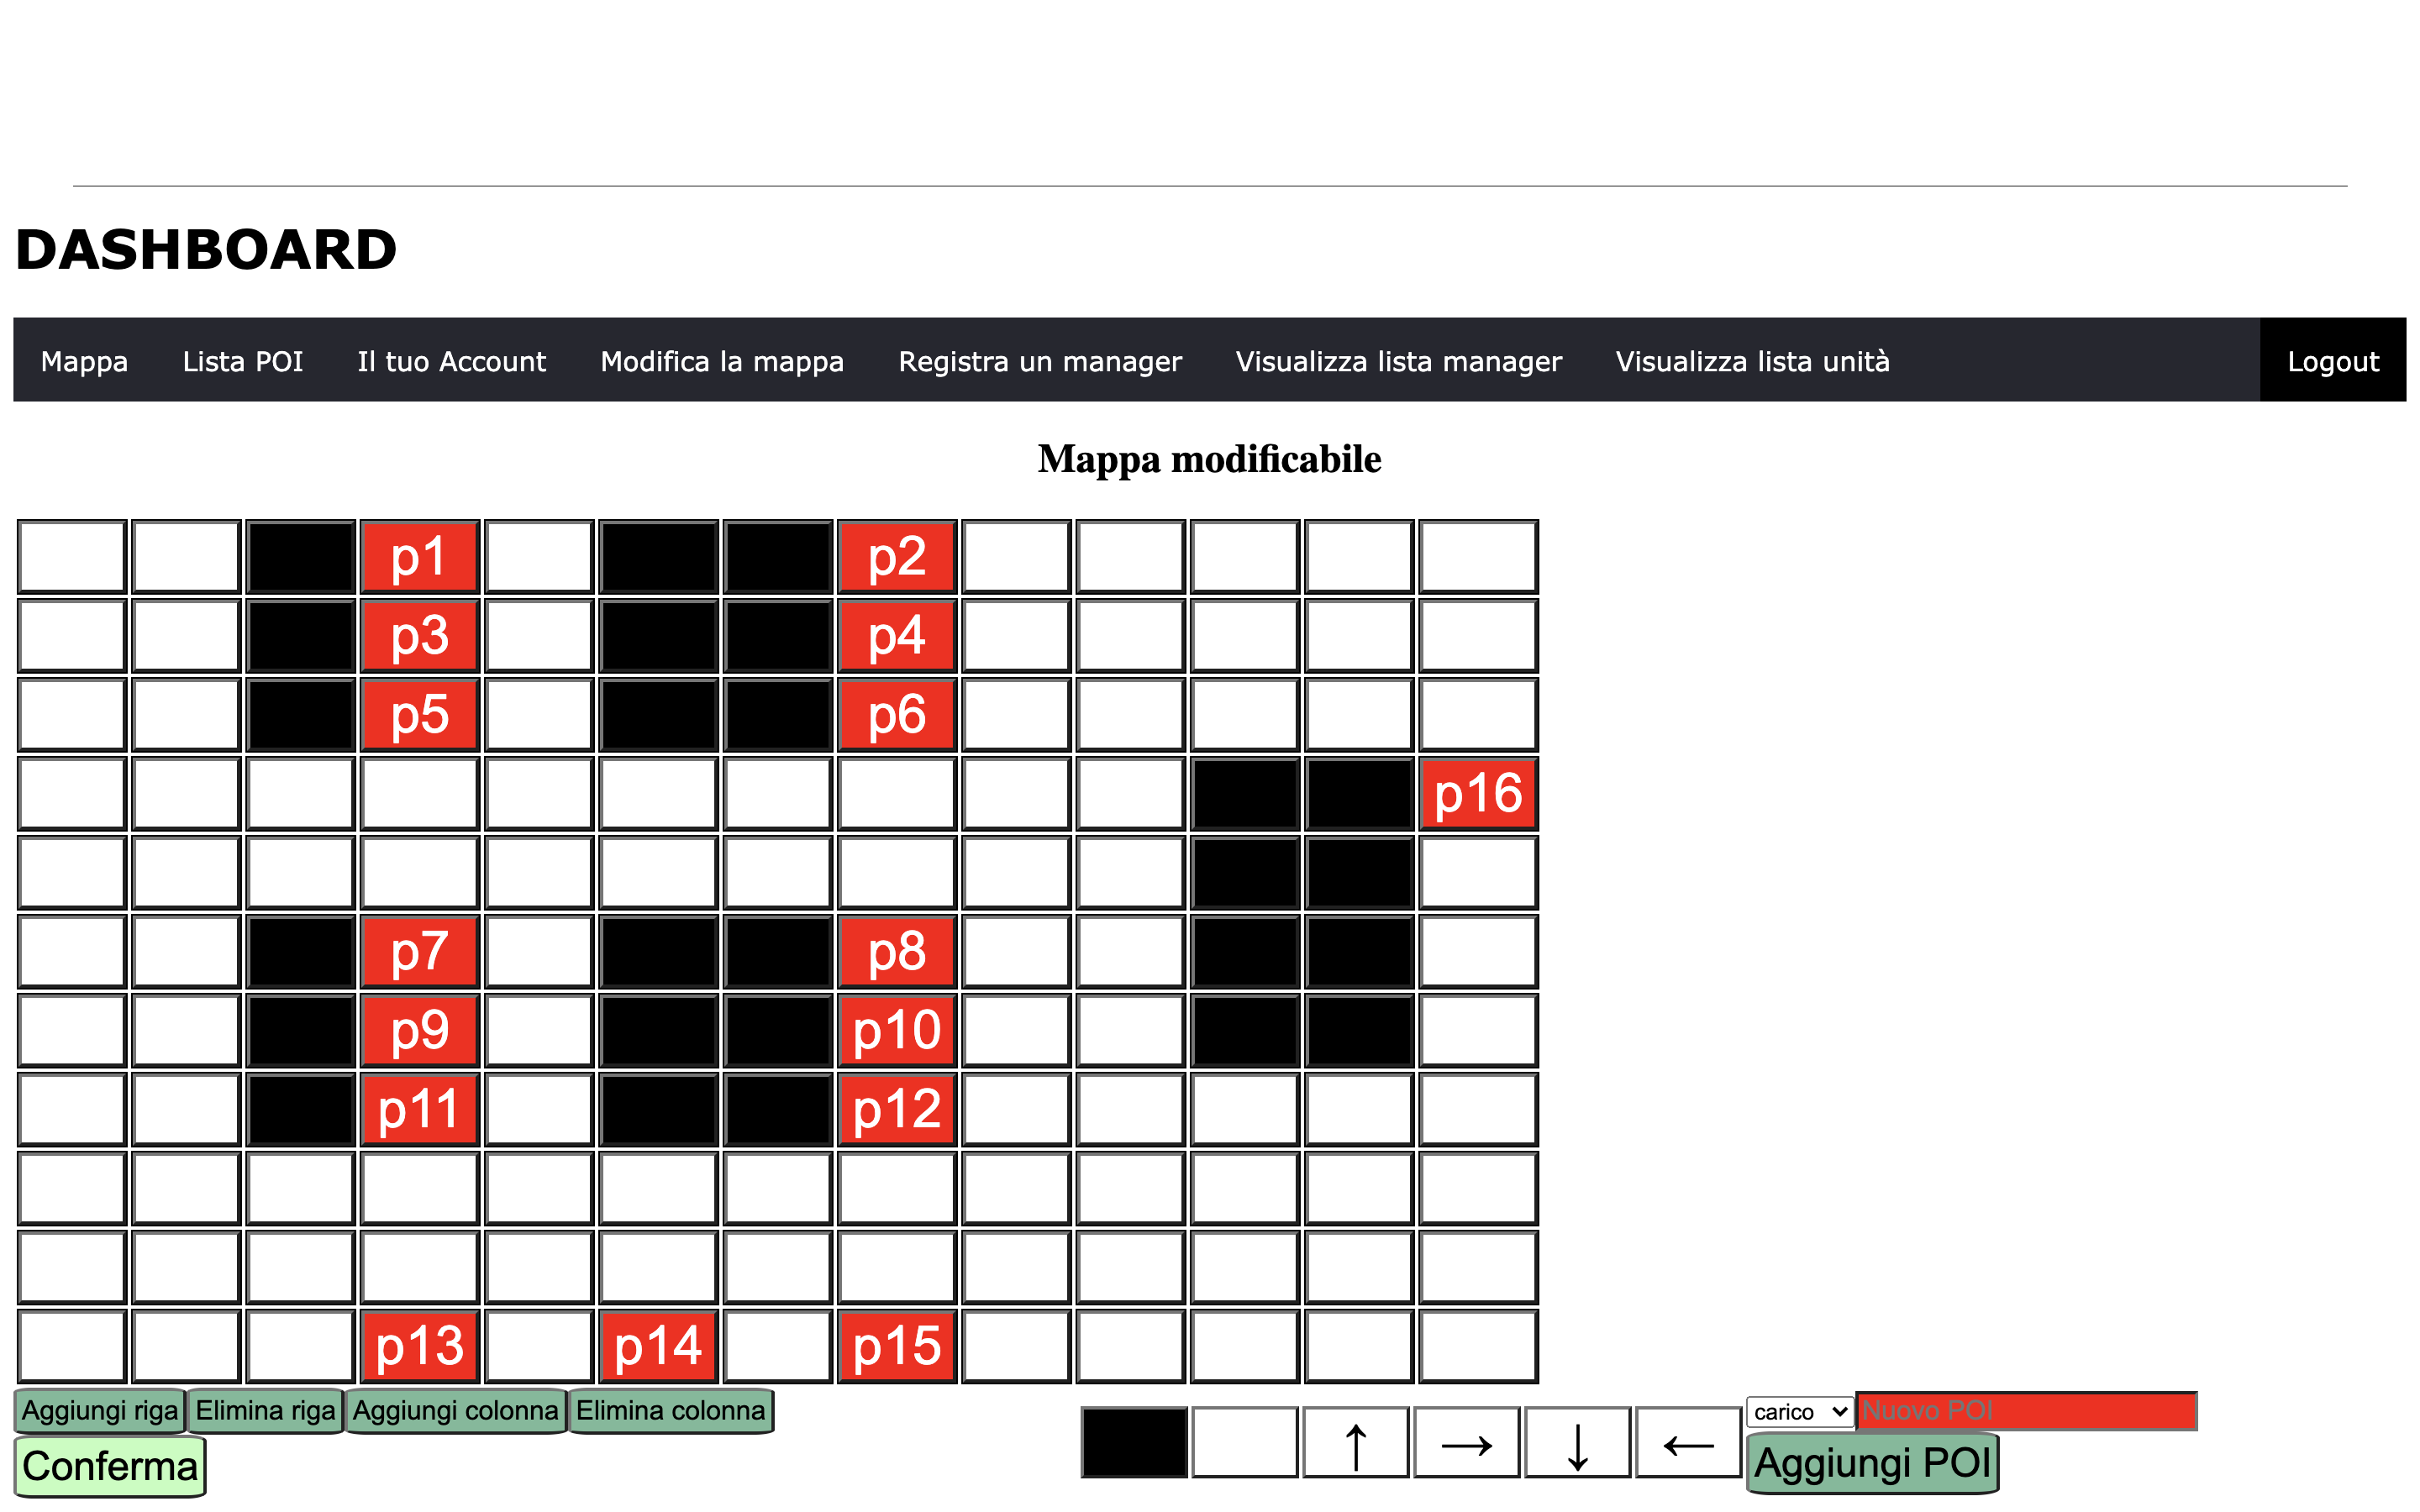
\includegraphics[scale=0.12]{res/images/managemap2.png}
            \caption{Schermata modifica mappa}
        \end{figure}
    \item quando si è soddisfatti delle modifiche premere sul pulsante "Conferma".
\end{itemize}

\begin{figure}[H]
    \centering
    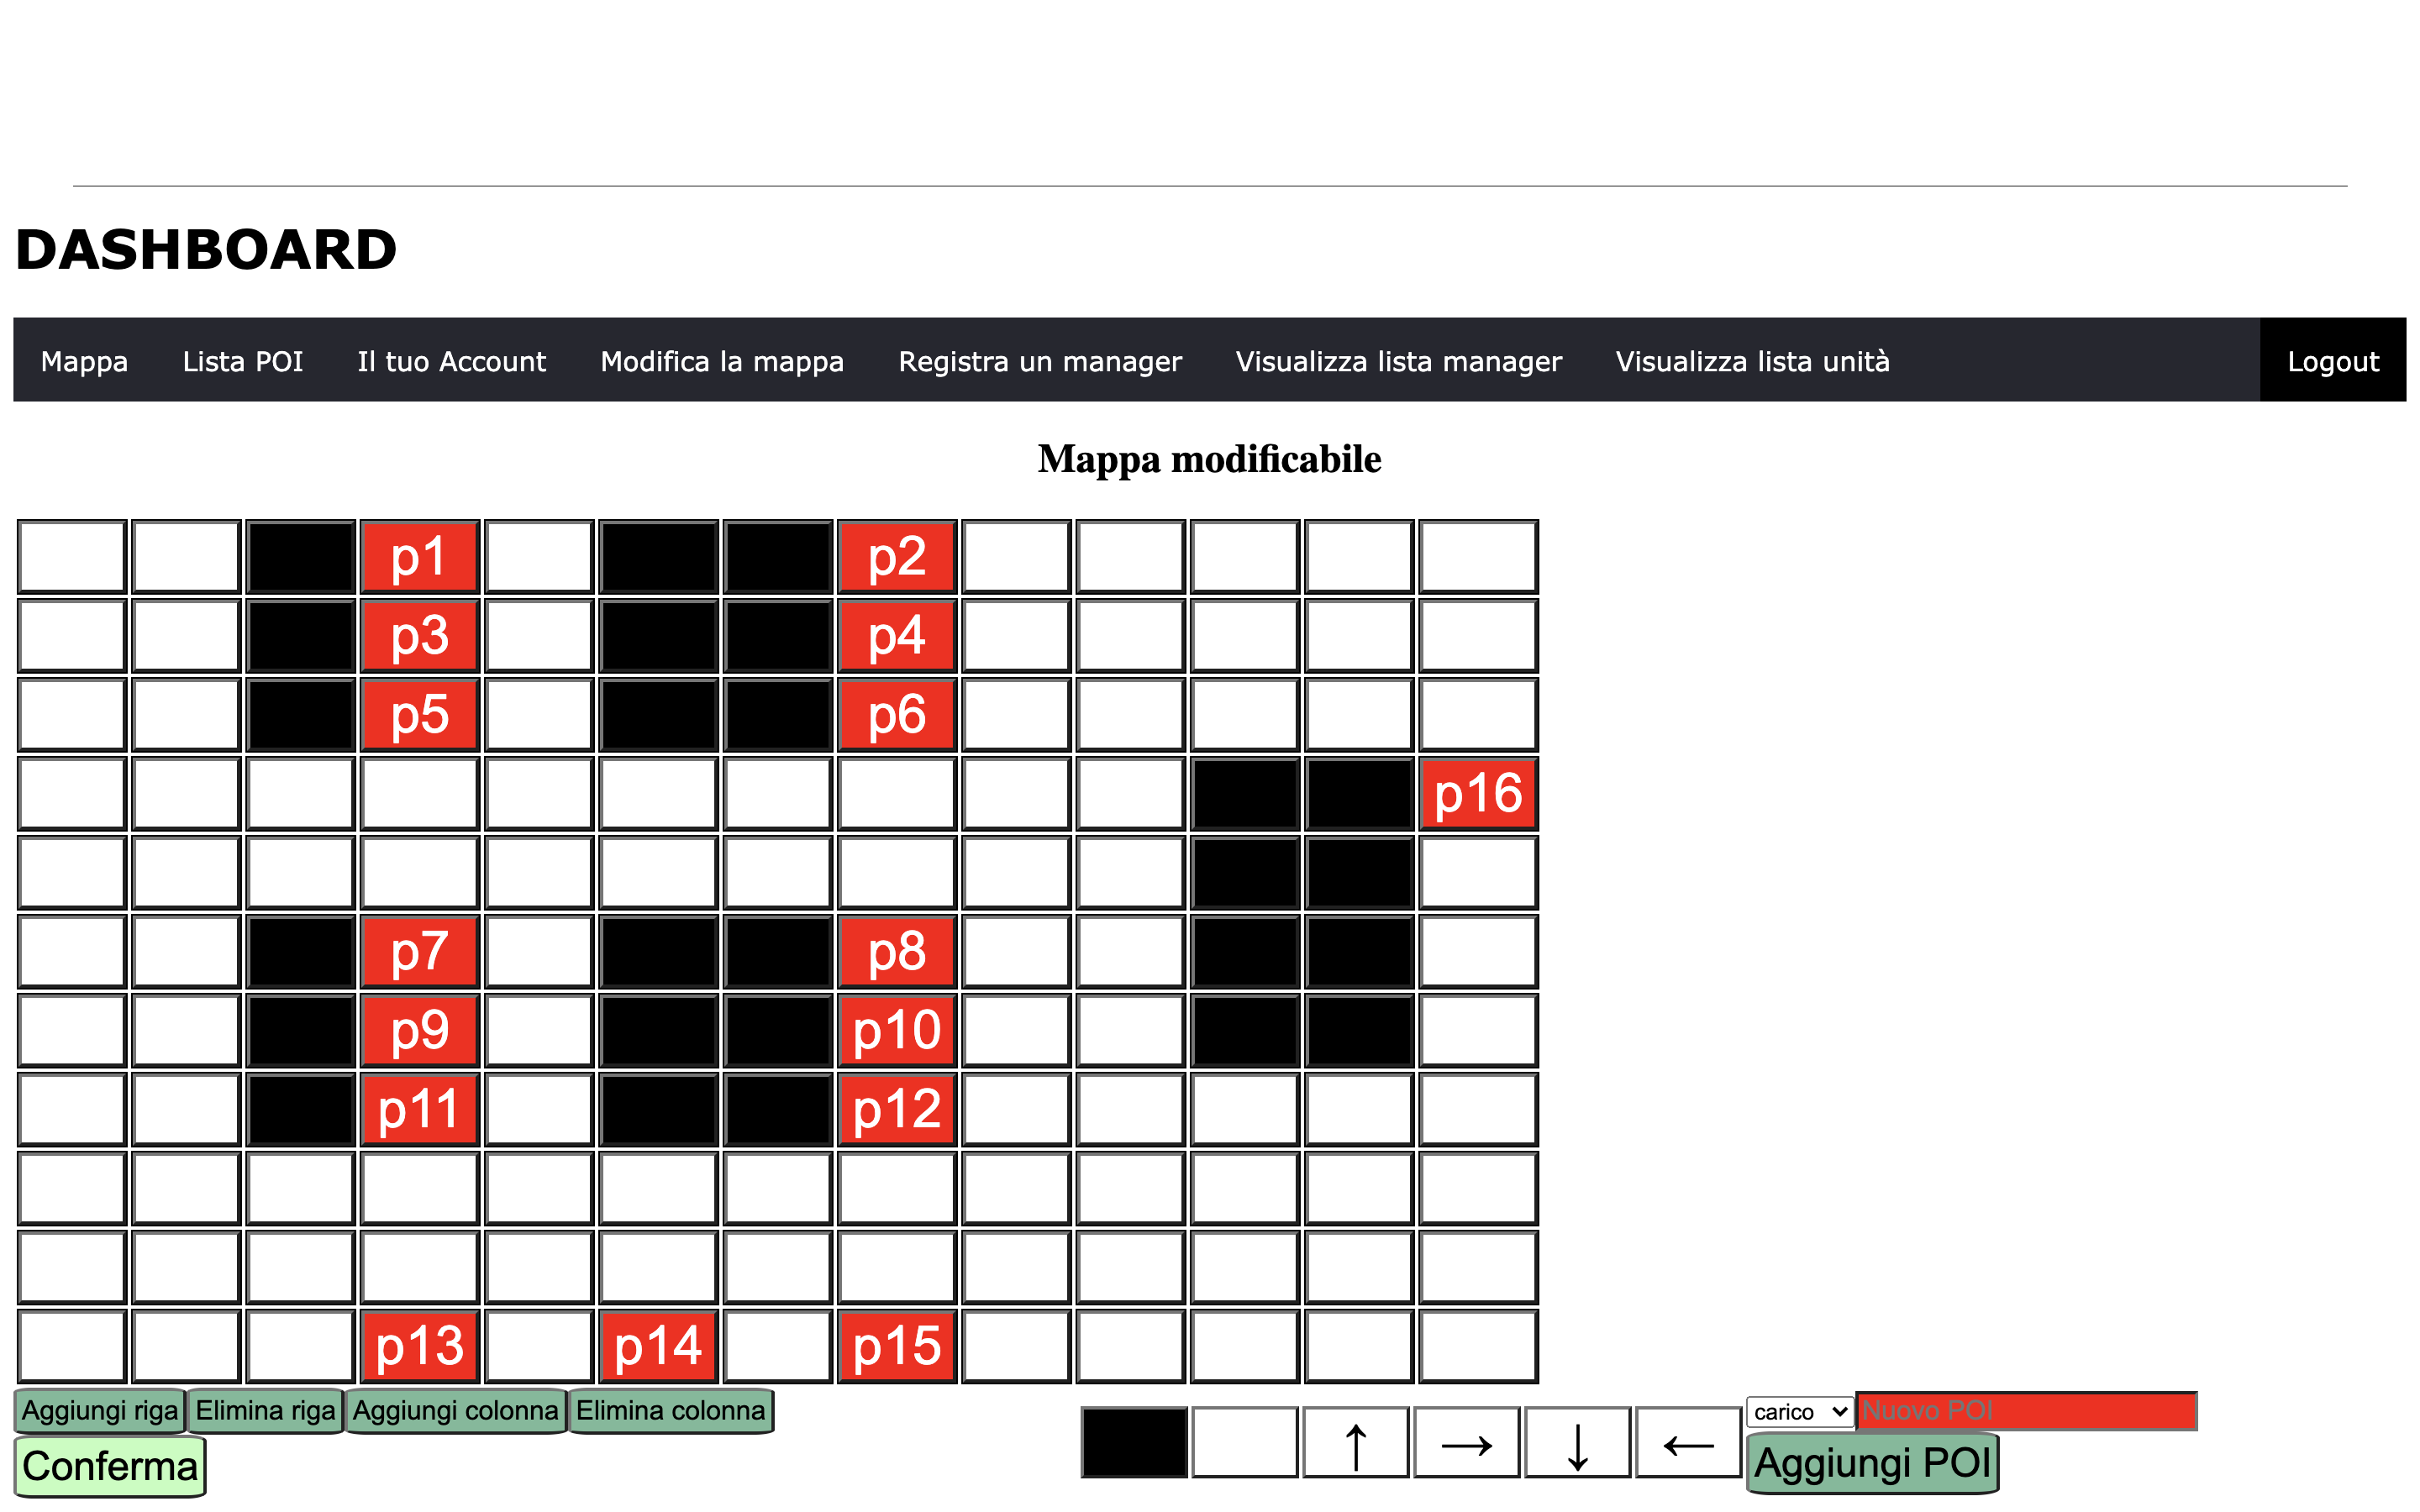
\includegraphics[scale=0.12]{res/images/managemap2.png}
    \caption{Schermata guida automatica dell'unità}
\end{figure}

\subsection{Gestione unità}
\begin{itemize}
\item Dopo l'autenticazione, tramite il menù selezionare il pulsante "Visualizza lista unità"; è possibile effettuare le seguenti operazioni:
    \item aggiungere una nuova unità: \\inserire il codice identificativo nel form e premere il pulsante "Registra";
    \item eliminare un'unità presente: 
    \begin{itemize}
        \item selezione dal menu a tendina l'id dell'untià che si intende eliminare;
        \item premere sul pulsante "Elimina" per confermare l'eliminazione.
    \end{itemize}
\end{itemize}
\begin{figure}[H]
    \centering
    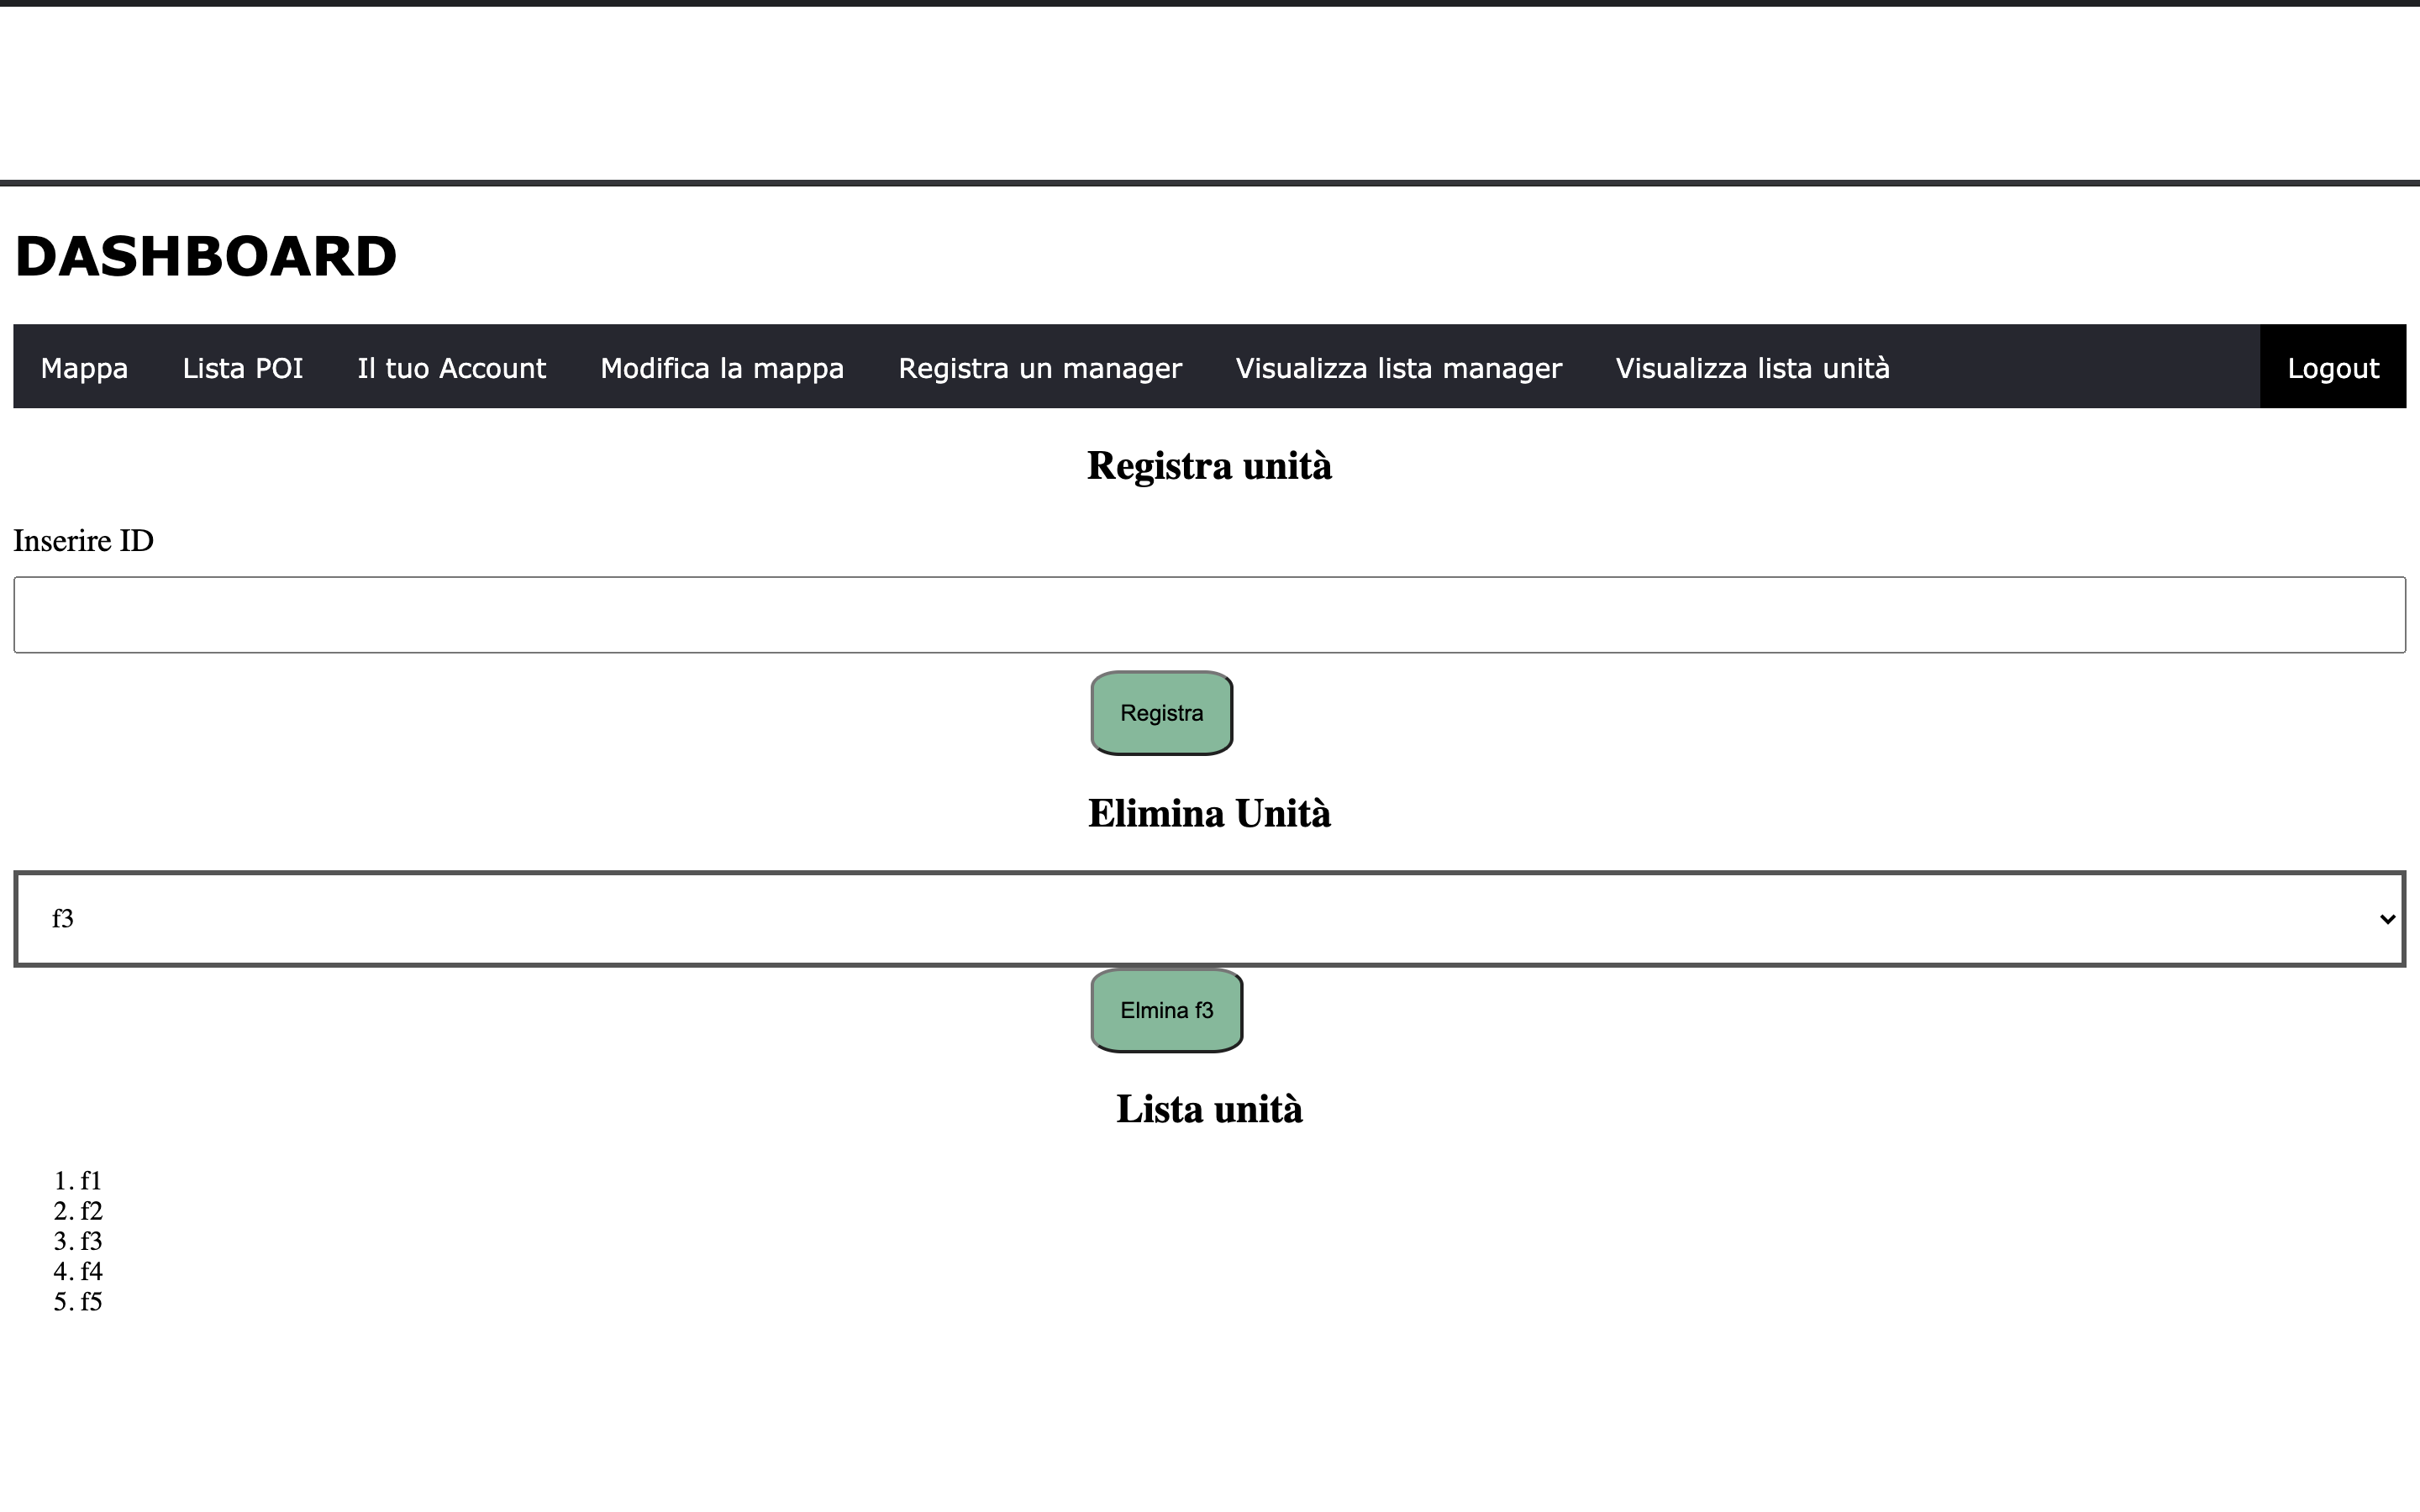
\includegraphics[scale=0.12]{res/images/newunit_admin.png}
    \caption{Schermata lista unità}
\end{figure}
	\pagebreak
	\section{Istruzione utilizzo utente responsabile}

La seguente sezione fornirà indicazioni utili per il corretto utilizzo del software nel caso l'utente interessato sia il responsabile.

\subsection{Login}
Il primo passo da effettuare è l'inserimento del proprio codice identificativo e password all'interno dei campi visualizzati nella pagina di login. Dopo aver premuto il pulsante di conferma, si verrà indirizzati alla pagina dedicata alle funzionalità di amministratore. Nel caso le credenziali inserite non risultino corrette, verrà visualizzato un messaggio d'errore e sarà quindi necessario inserire di nuovo i dati.
\begin{figure}[H]
    \centering
    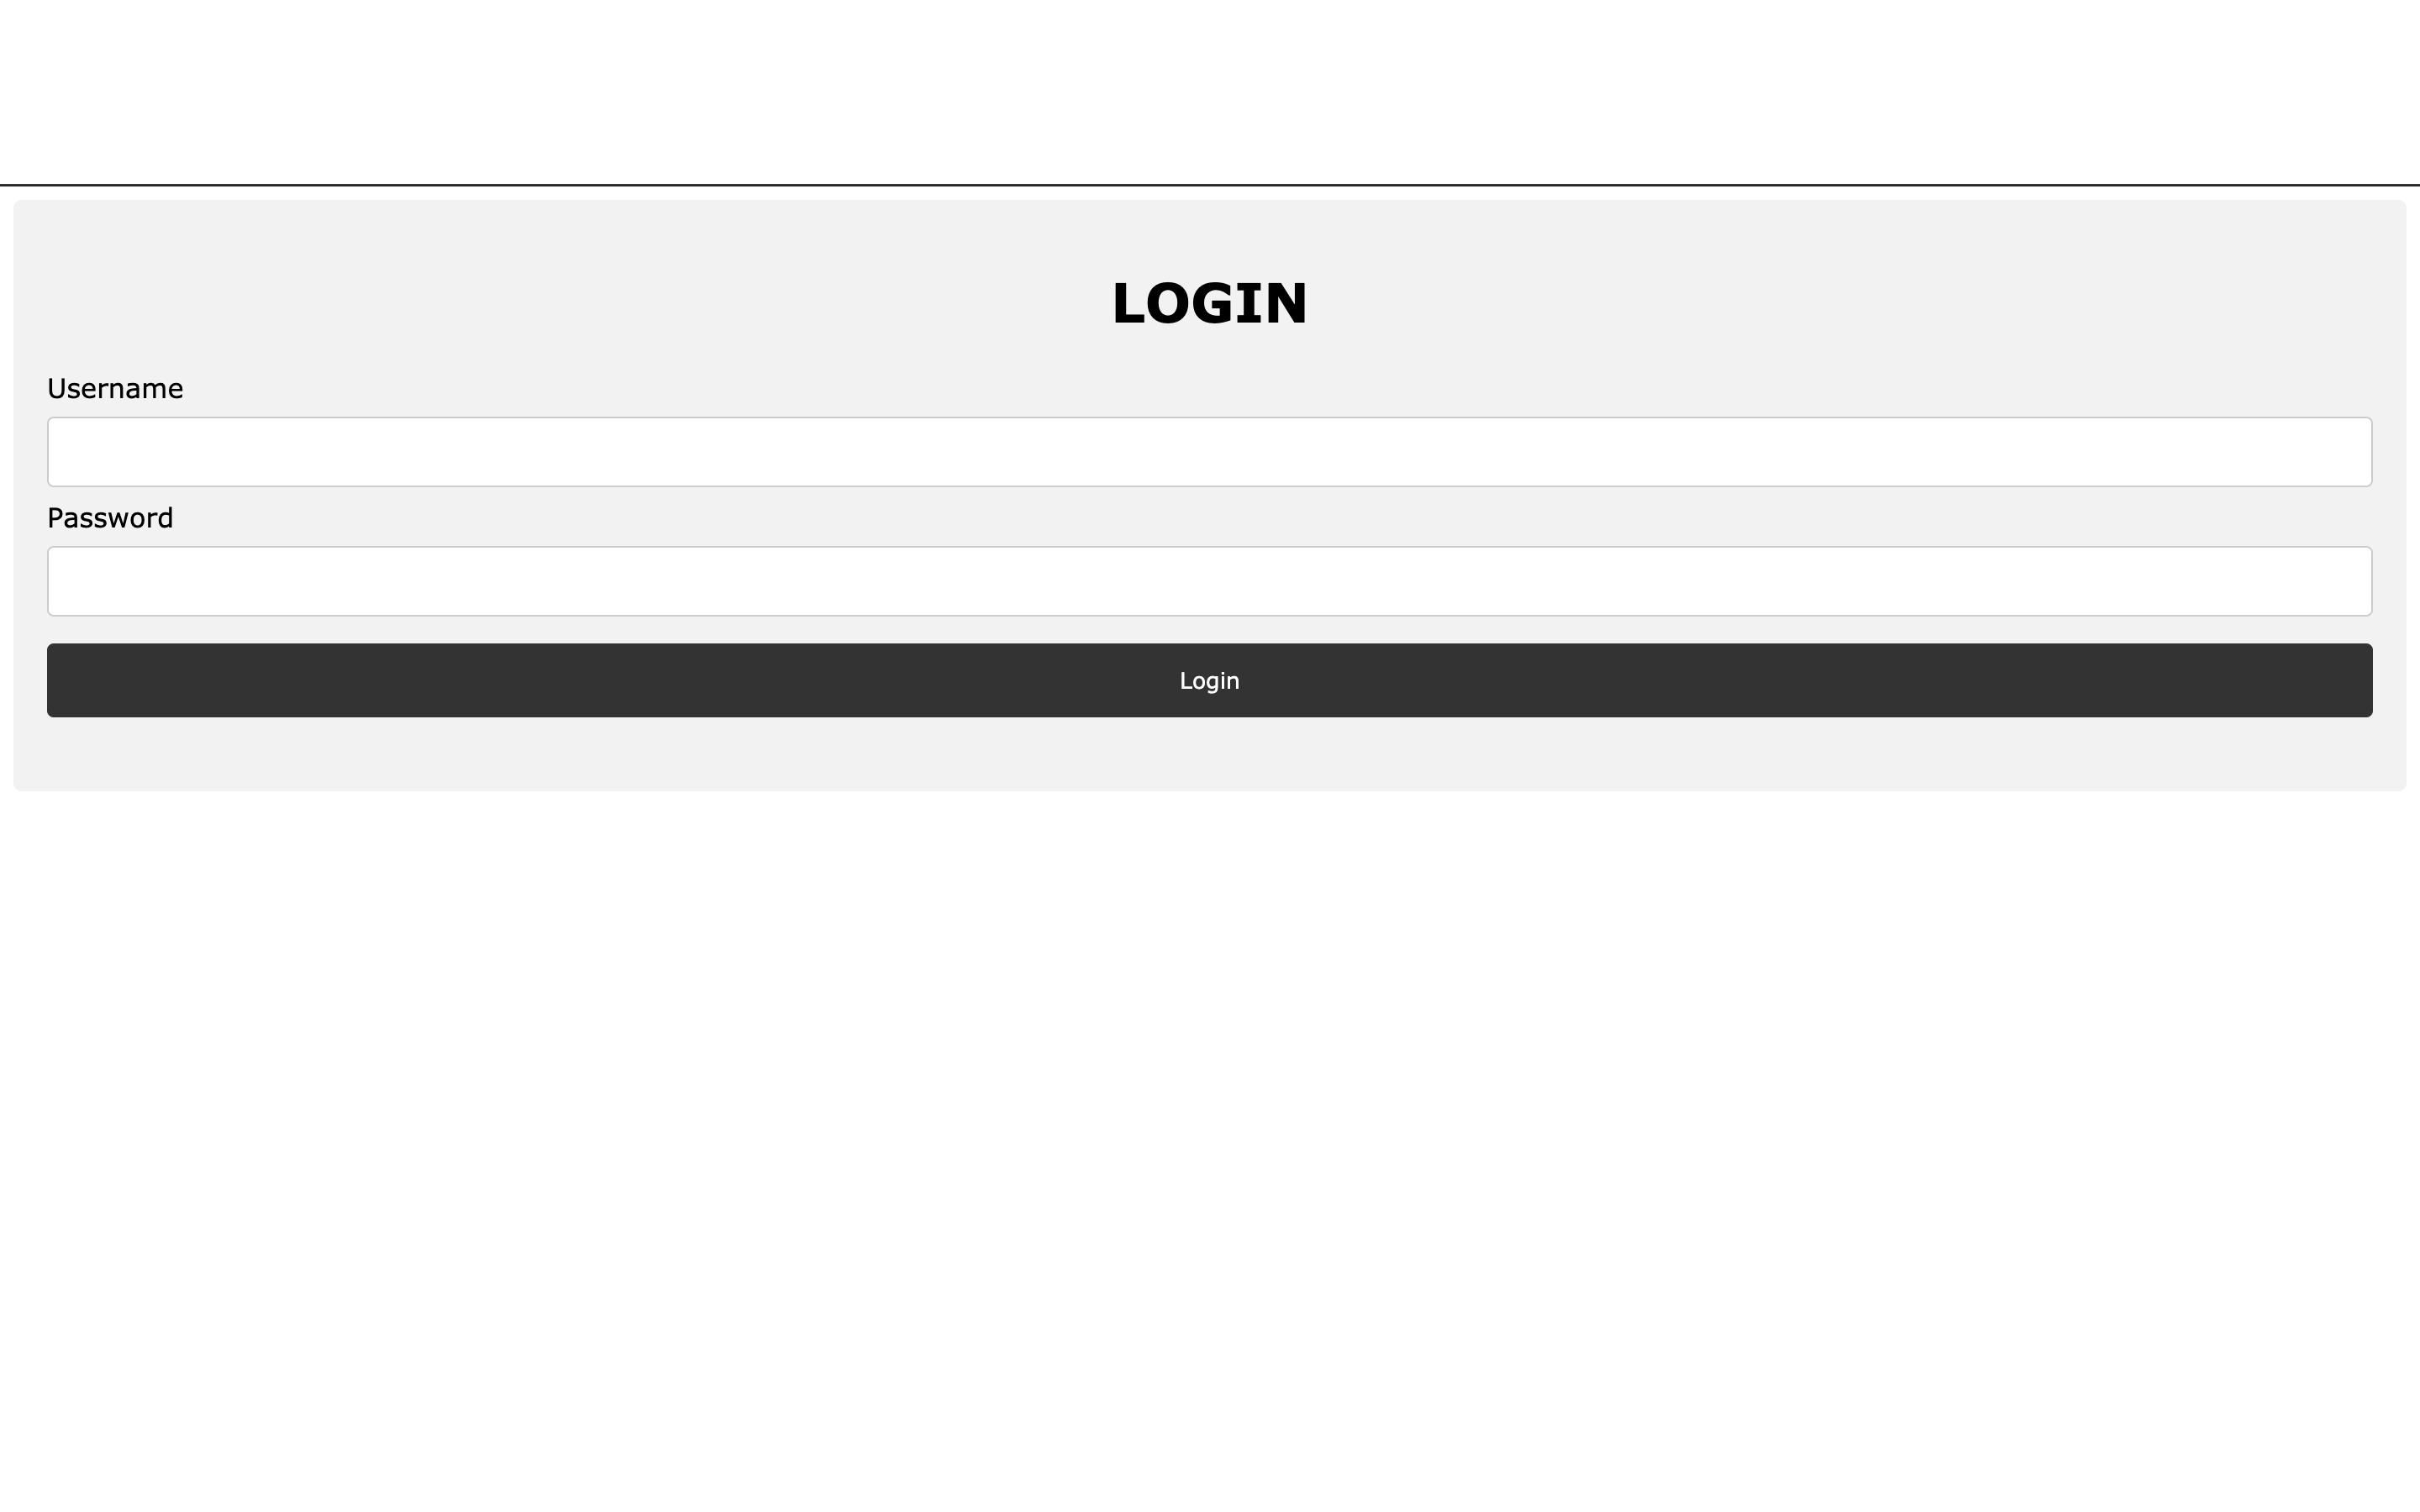
\includegraphics[scale=0.12]{res/images/login.png}
    \caption{Login}
\end{figure}

\subsection{Visualizzazione situazione in real time del magazzino}
\begin{itemize}
    \item Dopo l'autenticazione, tramite il menù selezionare il pulsante "Visualizza mappa";
    \item viene visualizzata la planimetria del magazzino con la relativa legenda e la rappresentazione dei muletti che si spostano;
    
\end{itemize}

\begin{figure}[H]
    \centering
    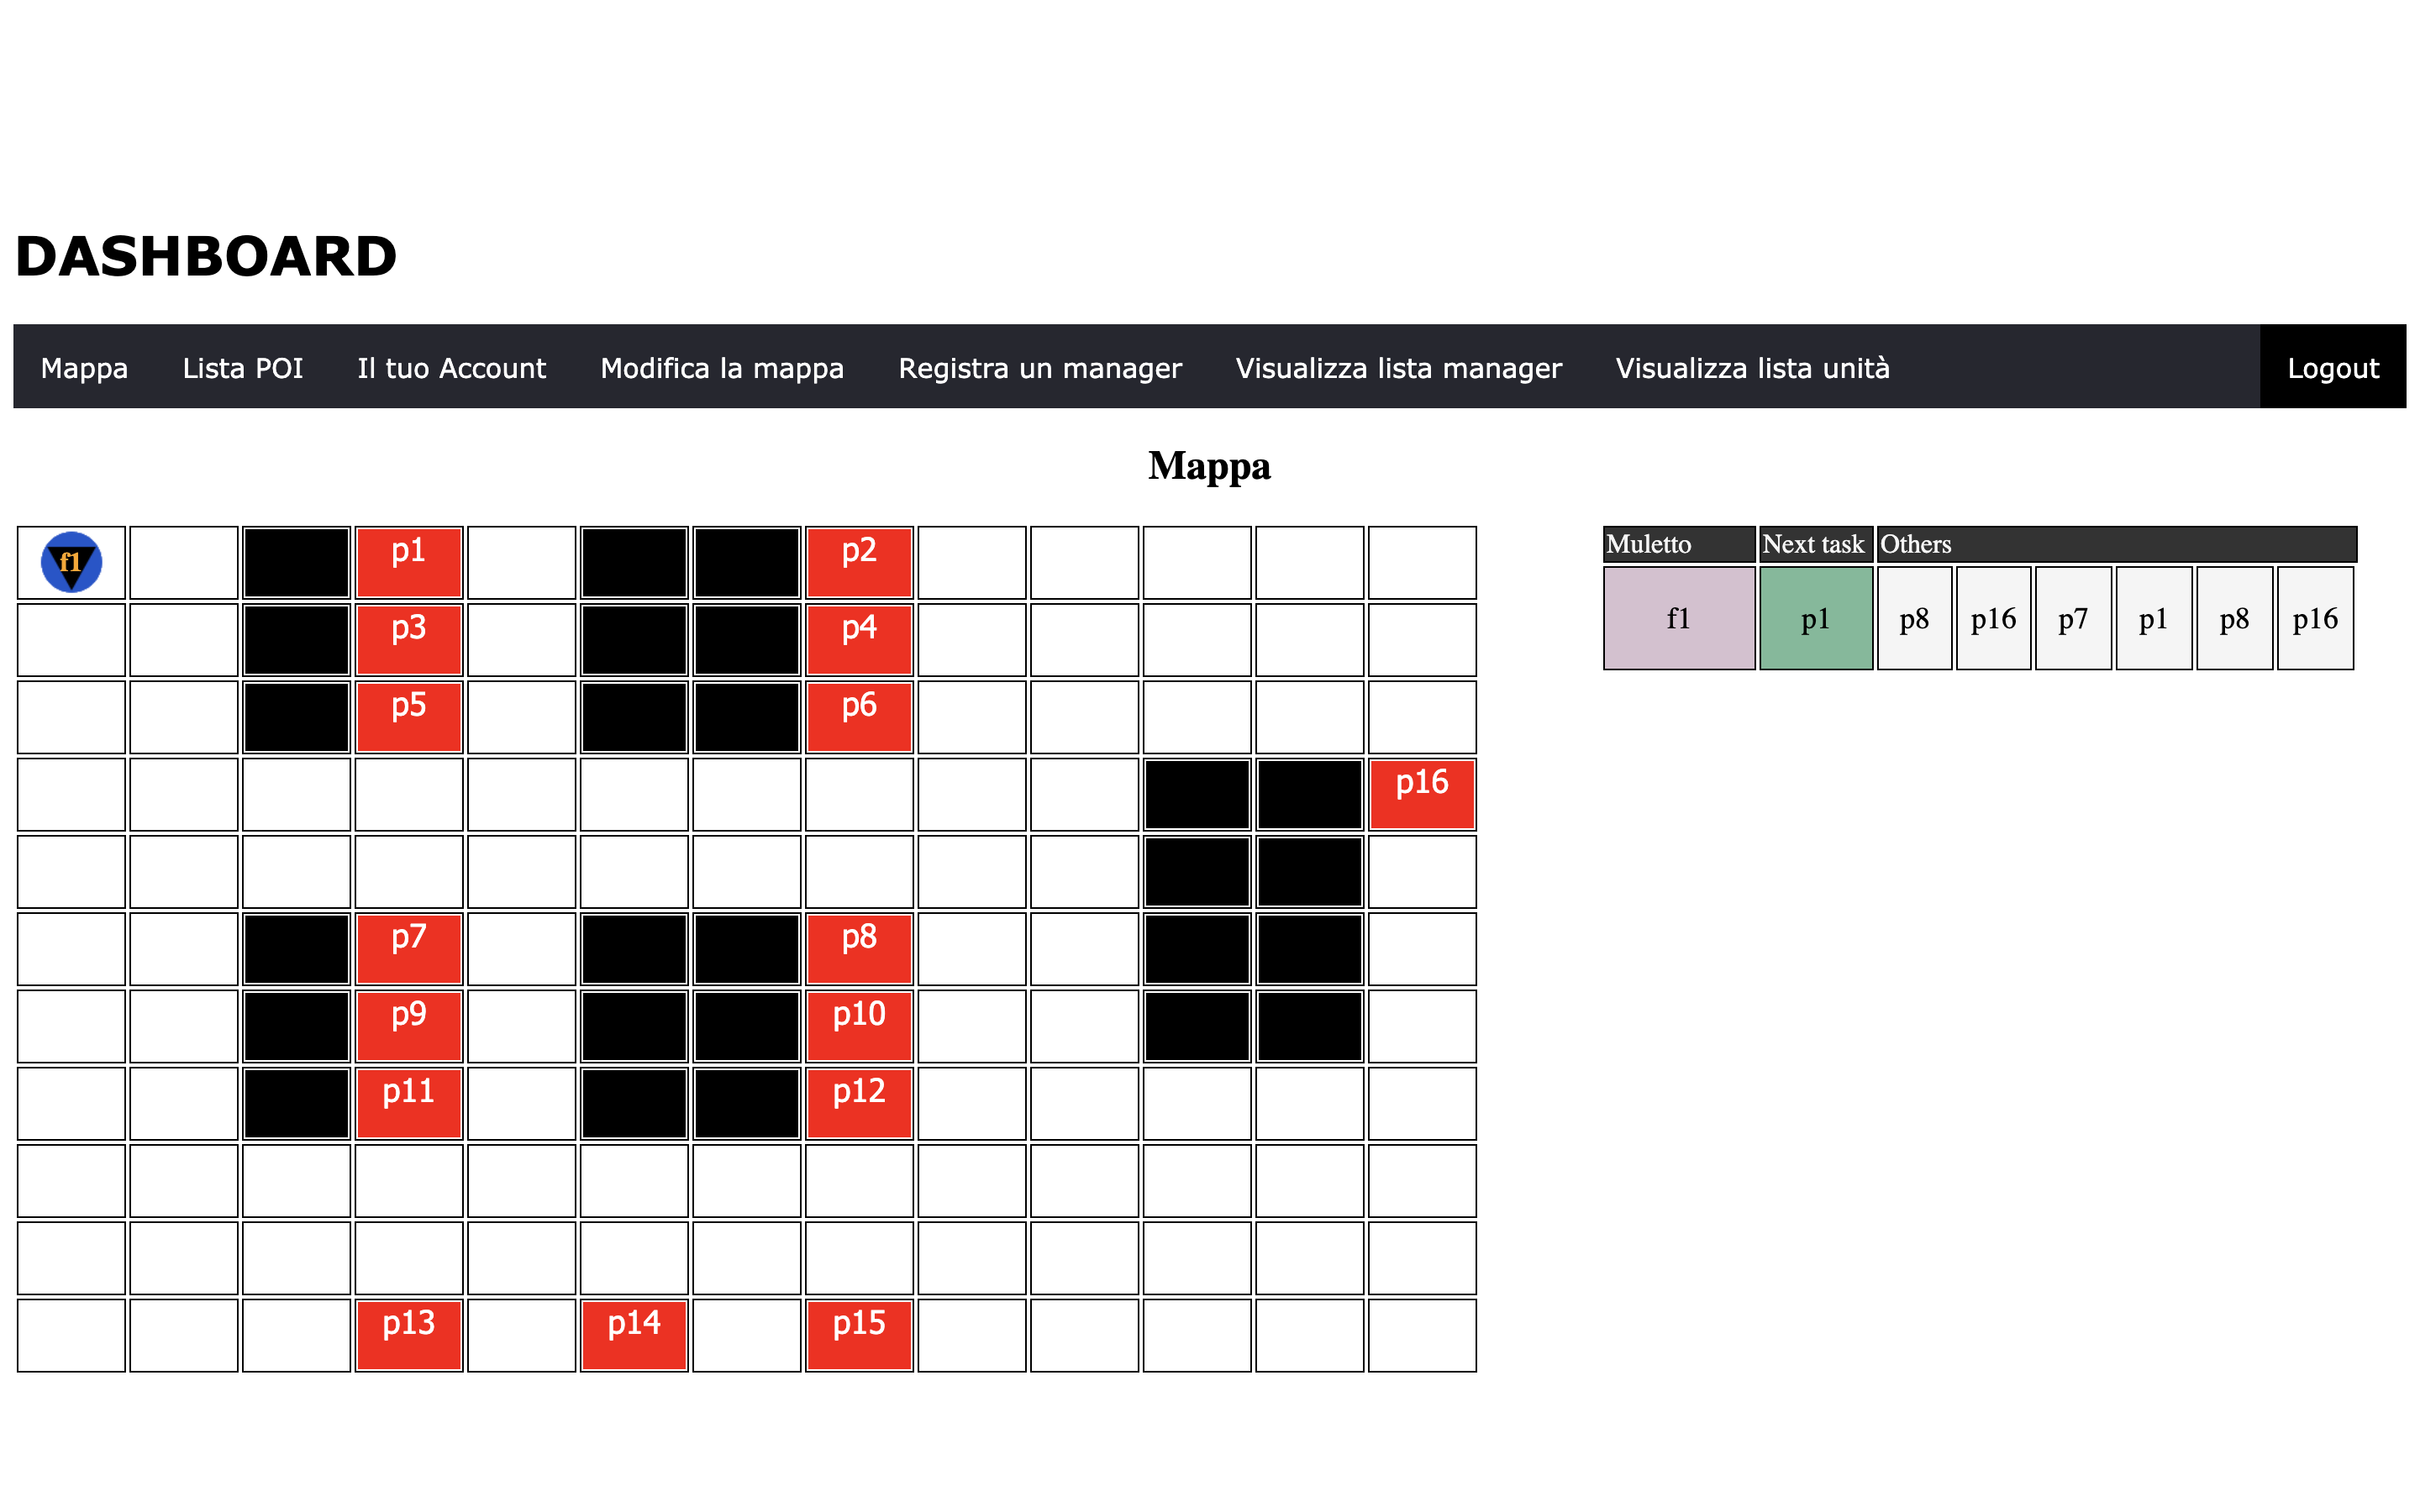
\includegraphics[scale=0.12]{res/images/map_user.png}
    \caption{Schermata guida automatica dell'unità}
\end{figure}

\subsection{Visualizzazione lista completa punti di interesse}
\begin{itemize}
    \item Dopo l'autenticazione, tramite il menù selezionare il pulsante "Visualizza lista POI";
    \item si viene indirizzati alla pagina con l'elenco di tutti i punti di interesse presenti nel magazzino;
    
\end{itemize}

\begin{figure}[H]
    \centering
    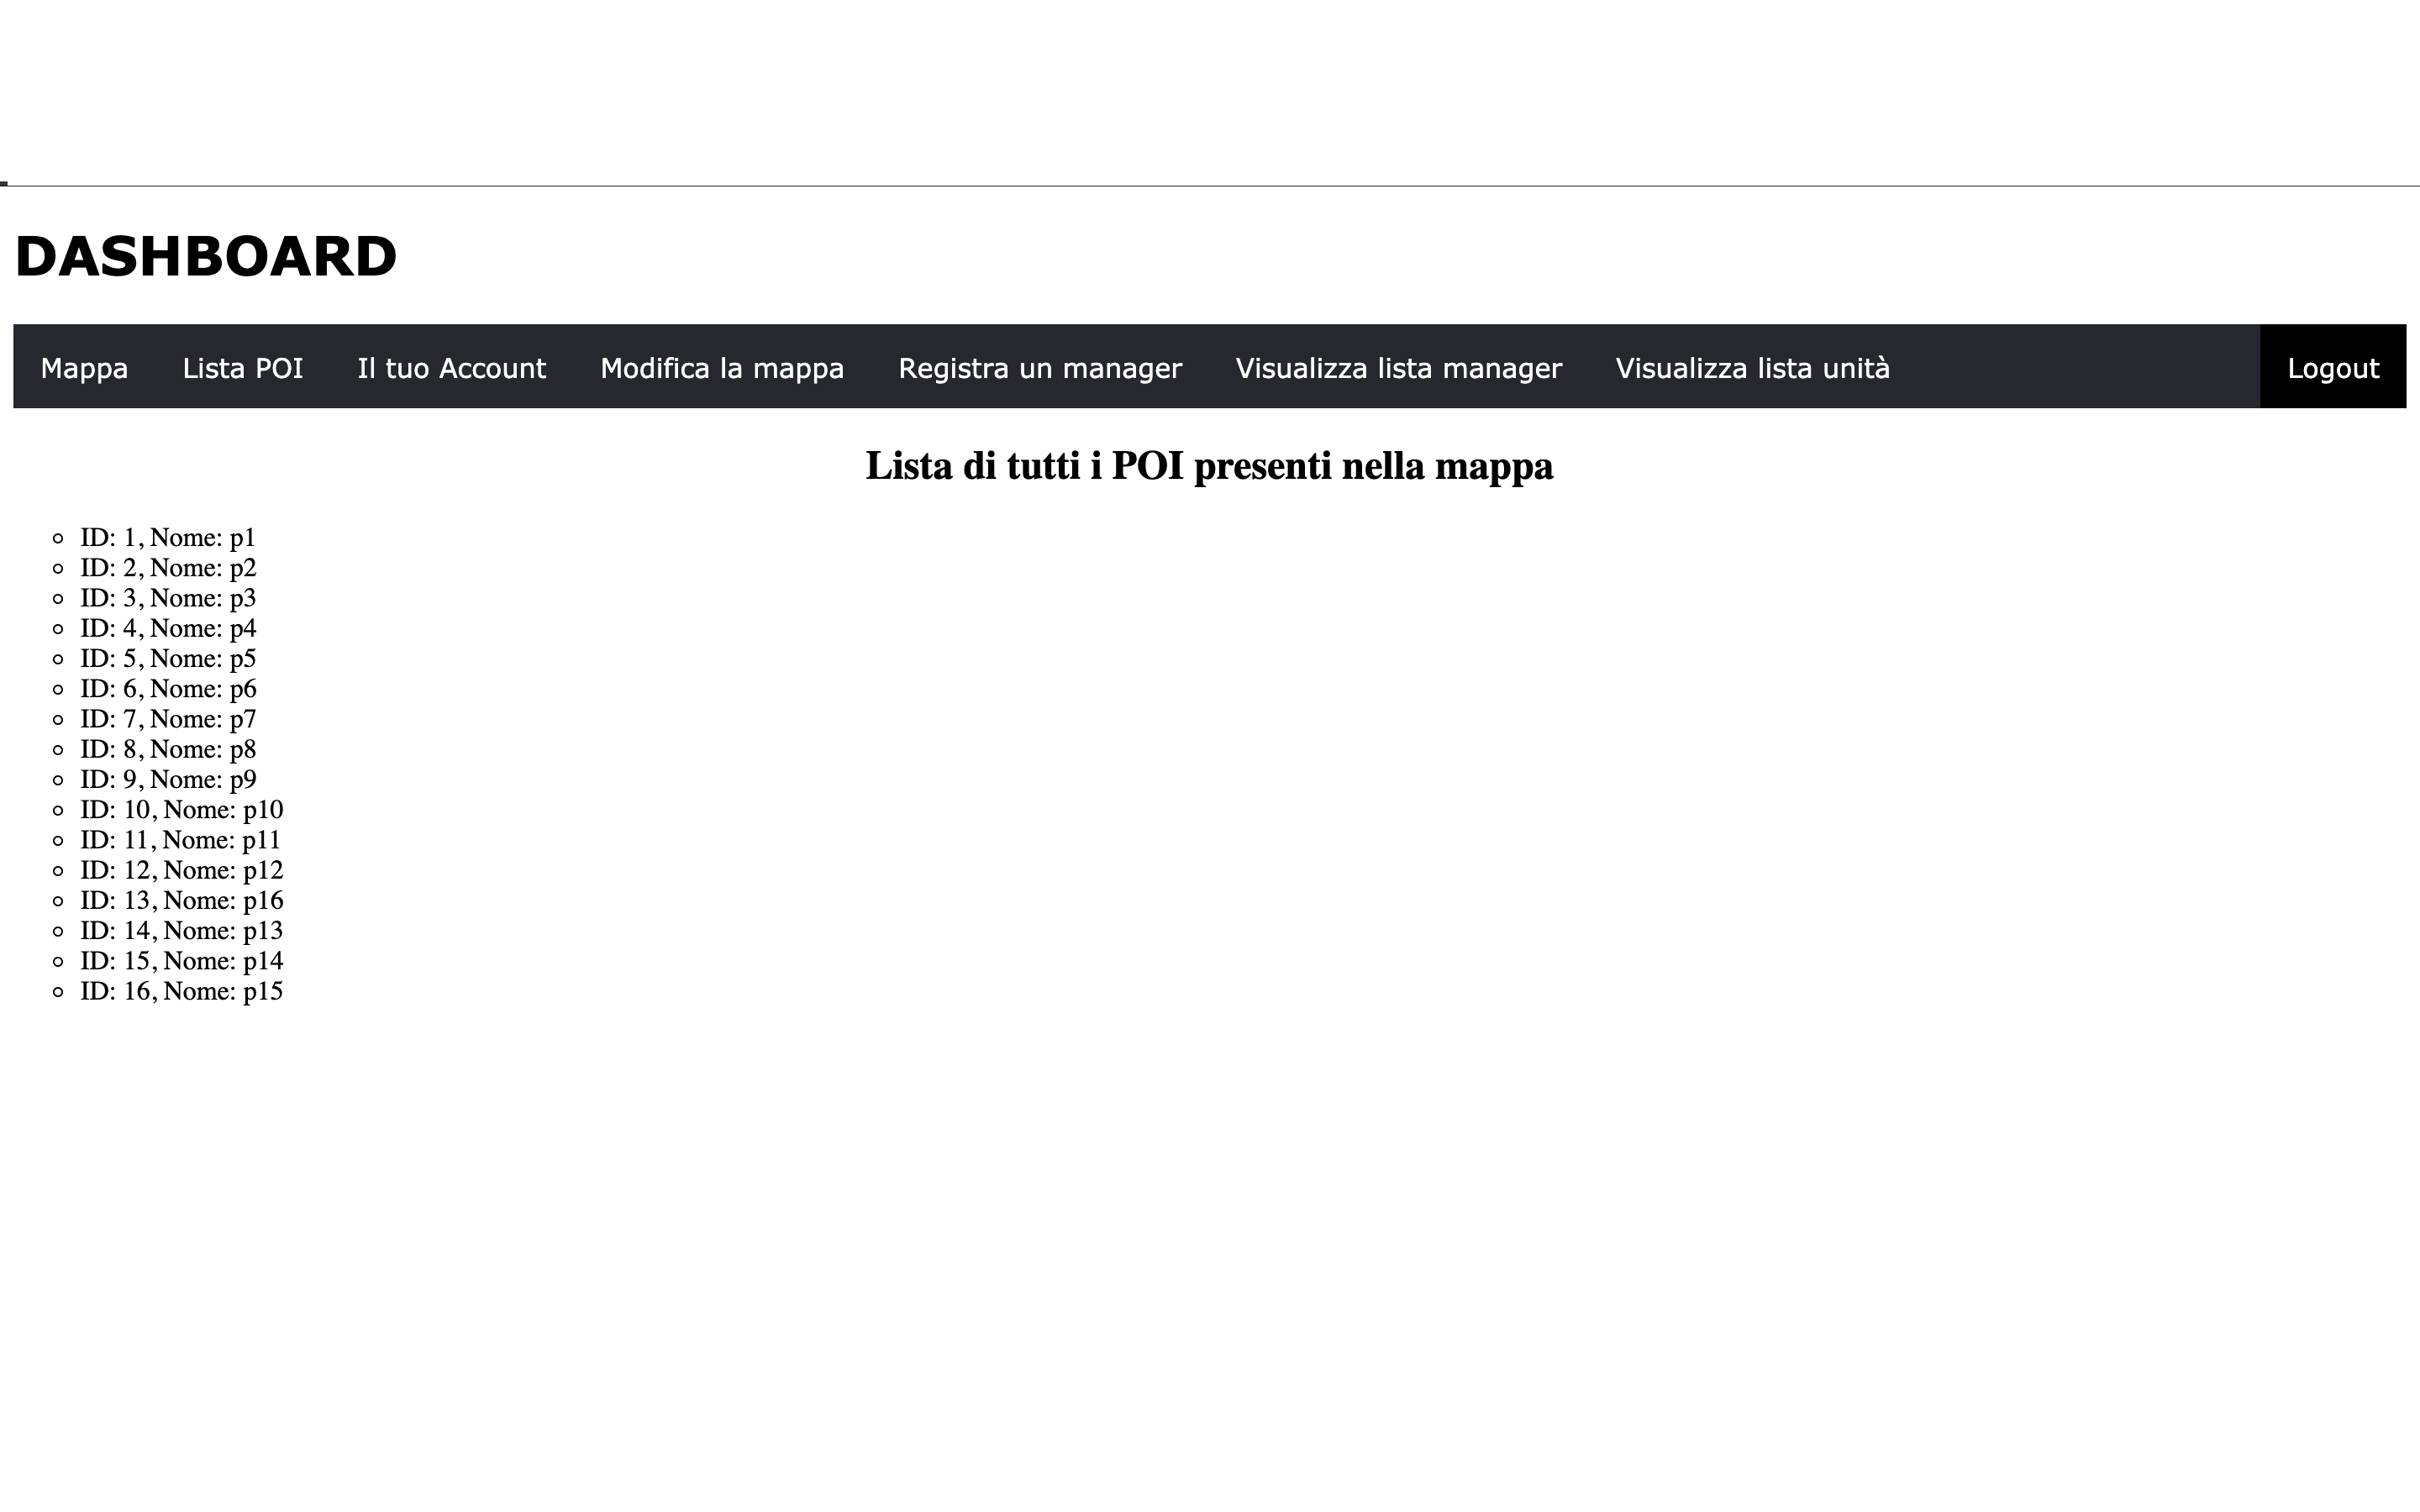
\includegraphics[scale=0.12]{res/images/listpoi_user.png}
    \caption{Schermata guida automatica dell'unità}
\end{figure}

\subsection{Visualizzazione dati del proprio profilo e modifica}
\begin{itemize}
    \item Dopo l'autenticazione, tramite il menù selezionare il pulsante "Visualizza il tuo account";
    \item si viene indirizzati alla pagina con i propri dati utente: nome, cognome, password;
    \item se si desidera modificare alcuni campi, è necessario scrivere nell'apposito form i nuovi dati e premere il pulsante "Conferma";
    
\end{itemize}
\begin{figure}[H]
    \centering
    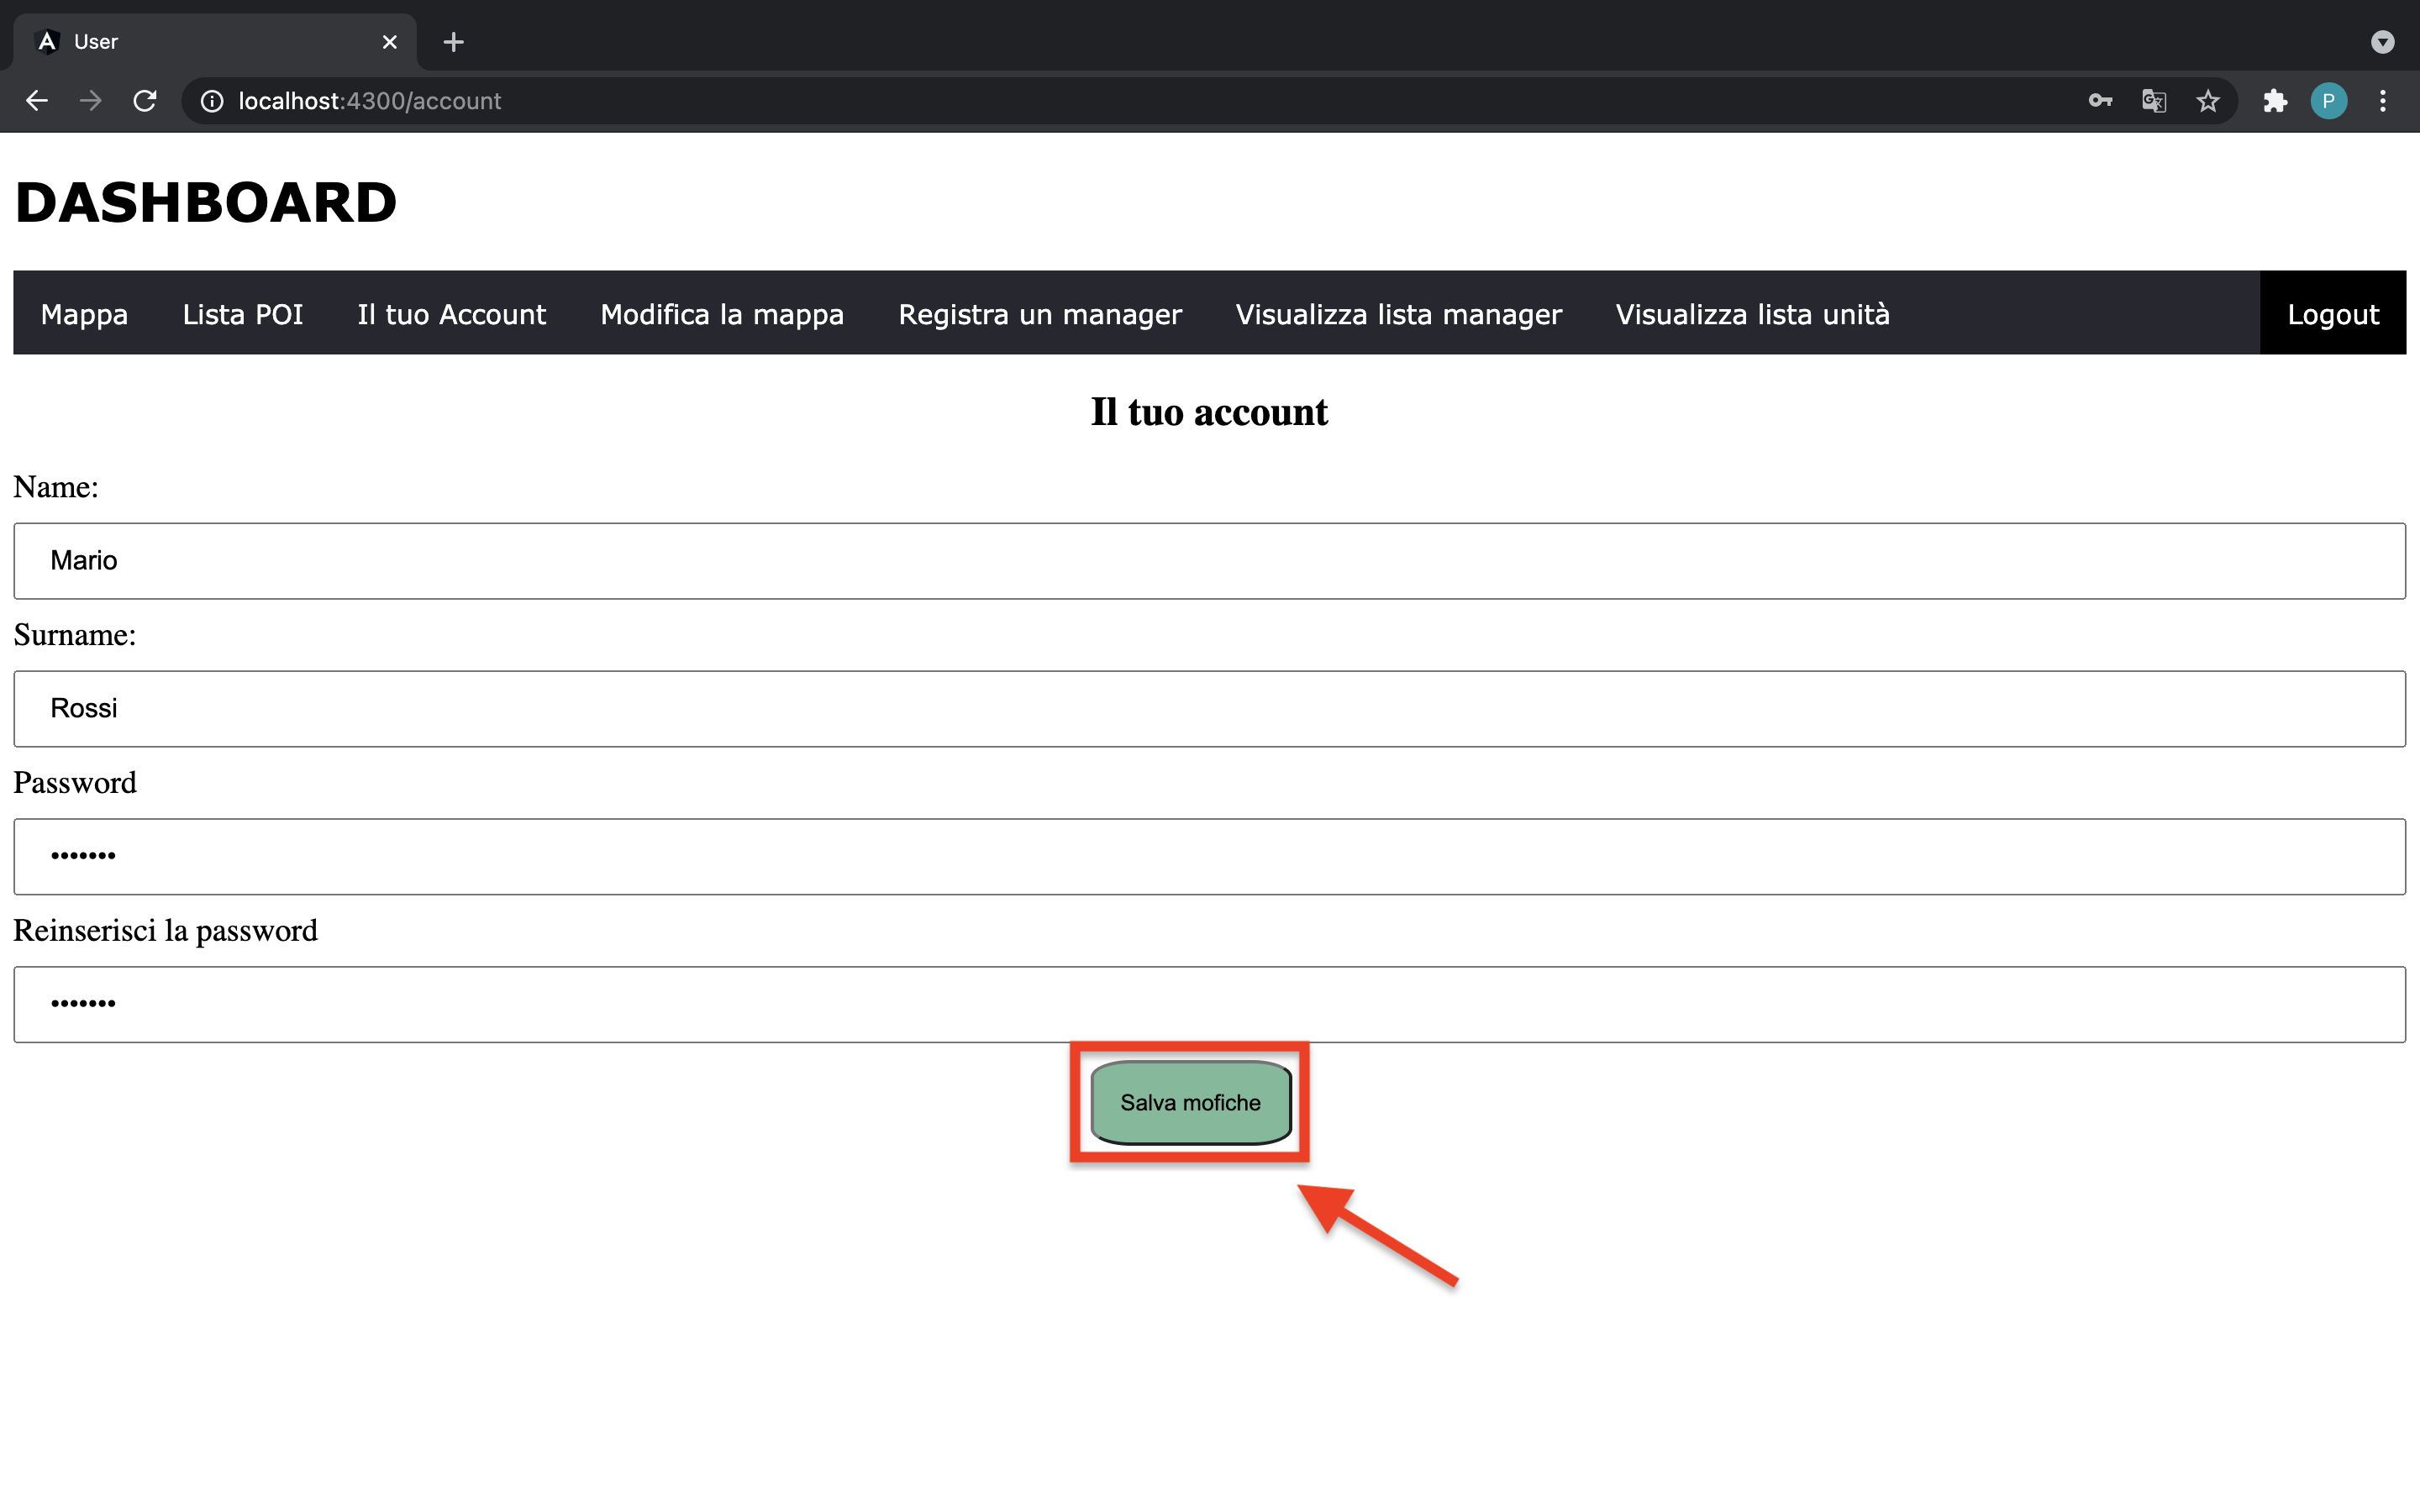
\includegraphics[scale=0.12]{res/images/account_user.png}
    \caption{Schermata guida automatica dell'unità}
\end{figure}

\subsection{Visualizzazione liste di task}
\begin{itemize}
    \item Dopo l'autenticazione, tramite il menù selezionare il pulsante "Visualizza liste di task";
    \item si viene indirizzati alla pagina con due liste: a sinistra le liste assegnate mentre a destra quelle non assegnate.

    
\end{itemize}
\begin{figure}[H]
    \centering
    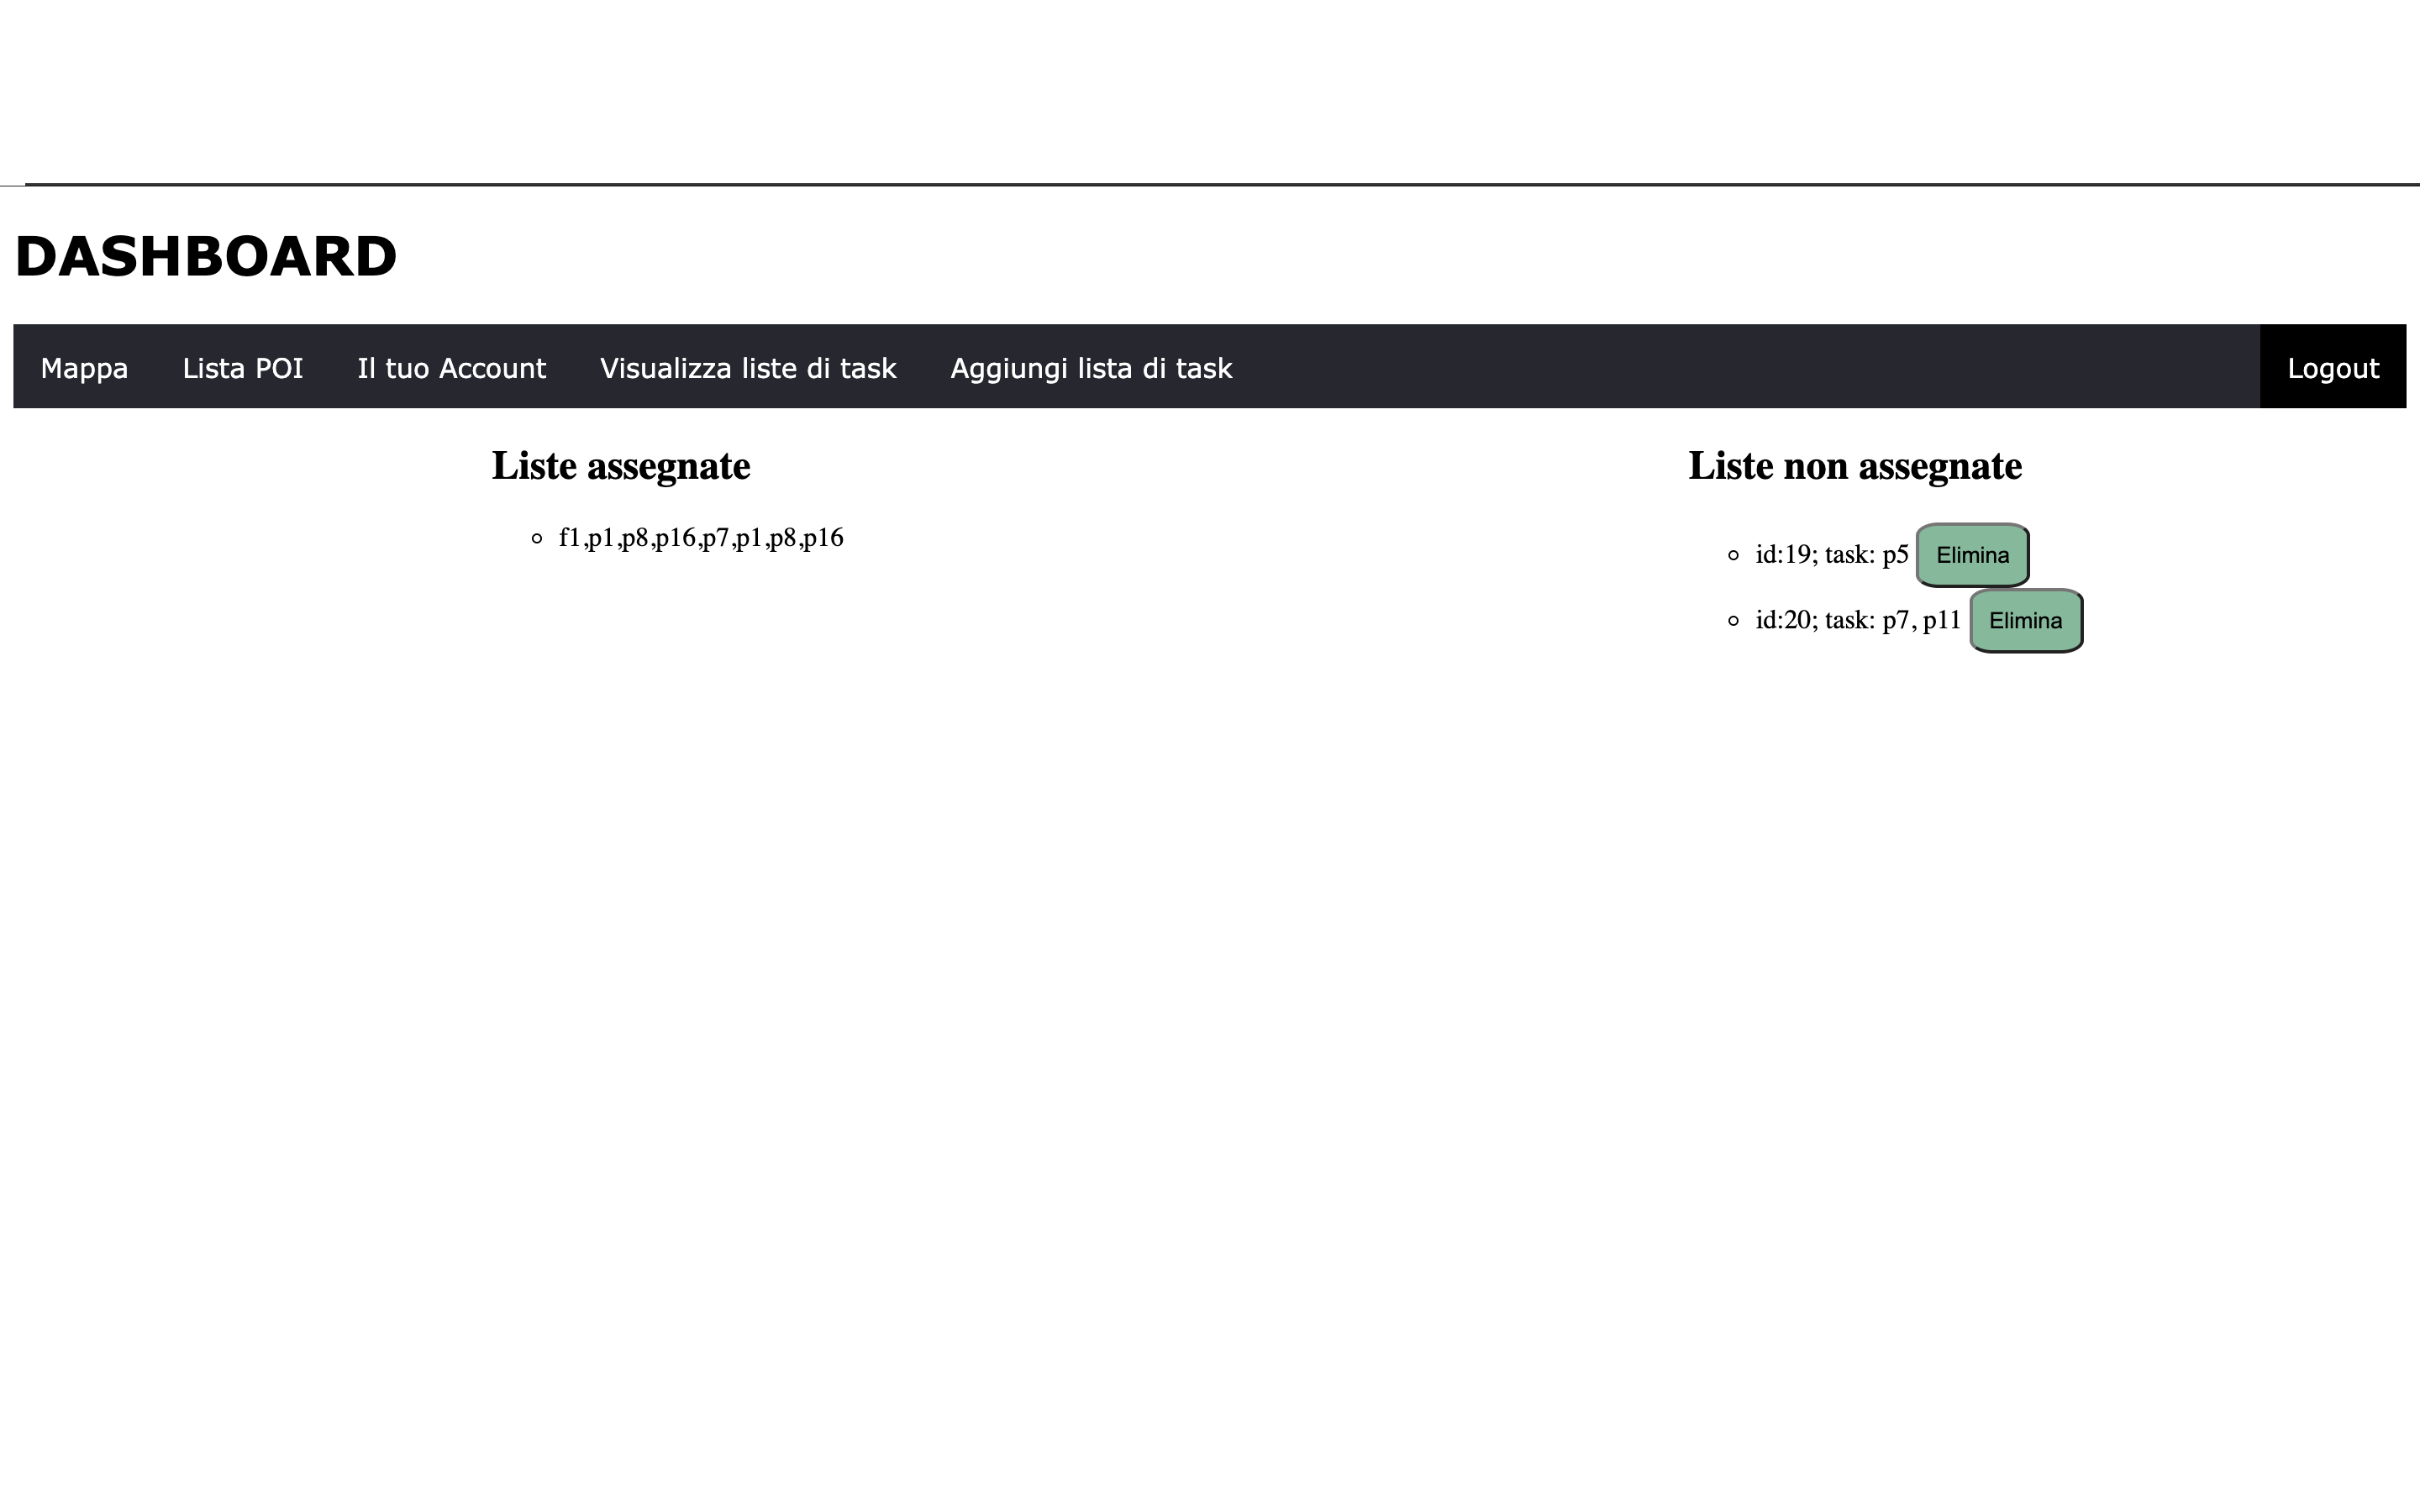
\includegraphics[scale=0.12]{res/images/task_manager.png}
    \caption{Schermata guida automatica dell'unità}
\end{figure}
\subsection{Gestione task}
\begin{itemize}
    \item Dopo l'autenticazione, tramite il menù selezionare il pulsante "Gestisci task";
    \item si viene indirizzati alla pagina con le operazioni per la gestione delle task;
\end{itemize}
\subsubsection{Aggiungere nuova lista di task}
\begin{itemize}
    \item Premere sul pulsante "Aggiungi nuova lista di task"
    \item viene visualizzato un form in cui inserire il POI di interesse e confermare; \\ripetere questo punto per tutte le task che si intendono inserire;
    \item tramite il pulsante "Elimina" di fianco ad ogni task inserita è possibile eliminarla prima di confermare;
    \item una volta aggiunte tutte le task, premere il pulsante "Conferma";
    \item per tornare alla pagina iniziale serve premere sul pulsante "Chiudi".
\end{itemize}

\begin{figure}[H]
    \centering
    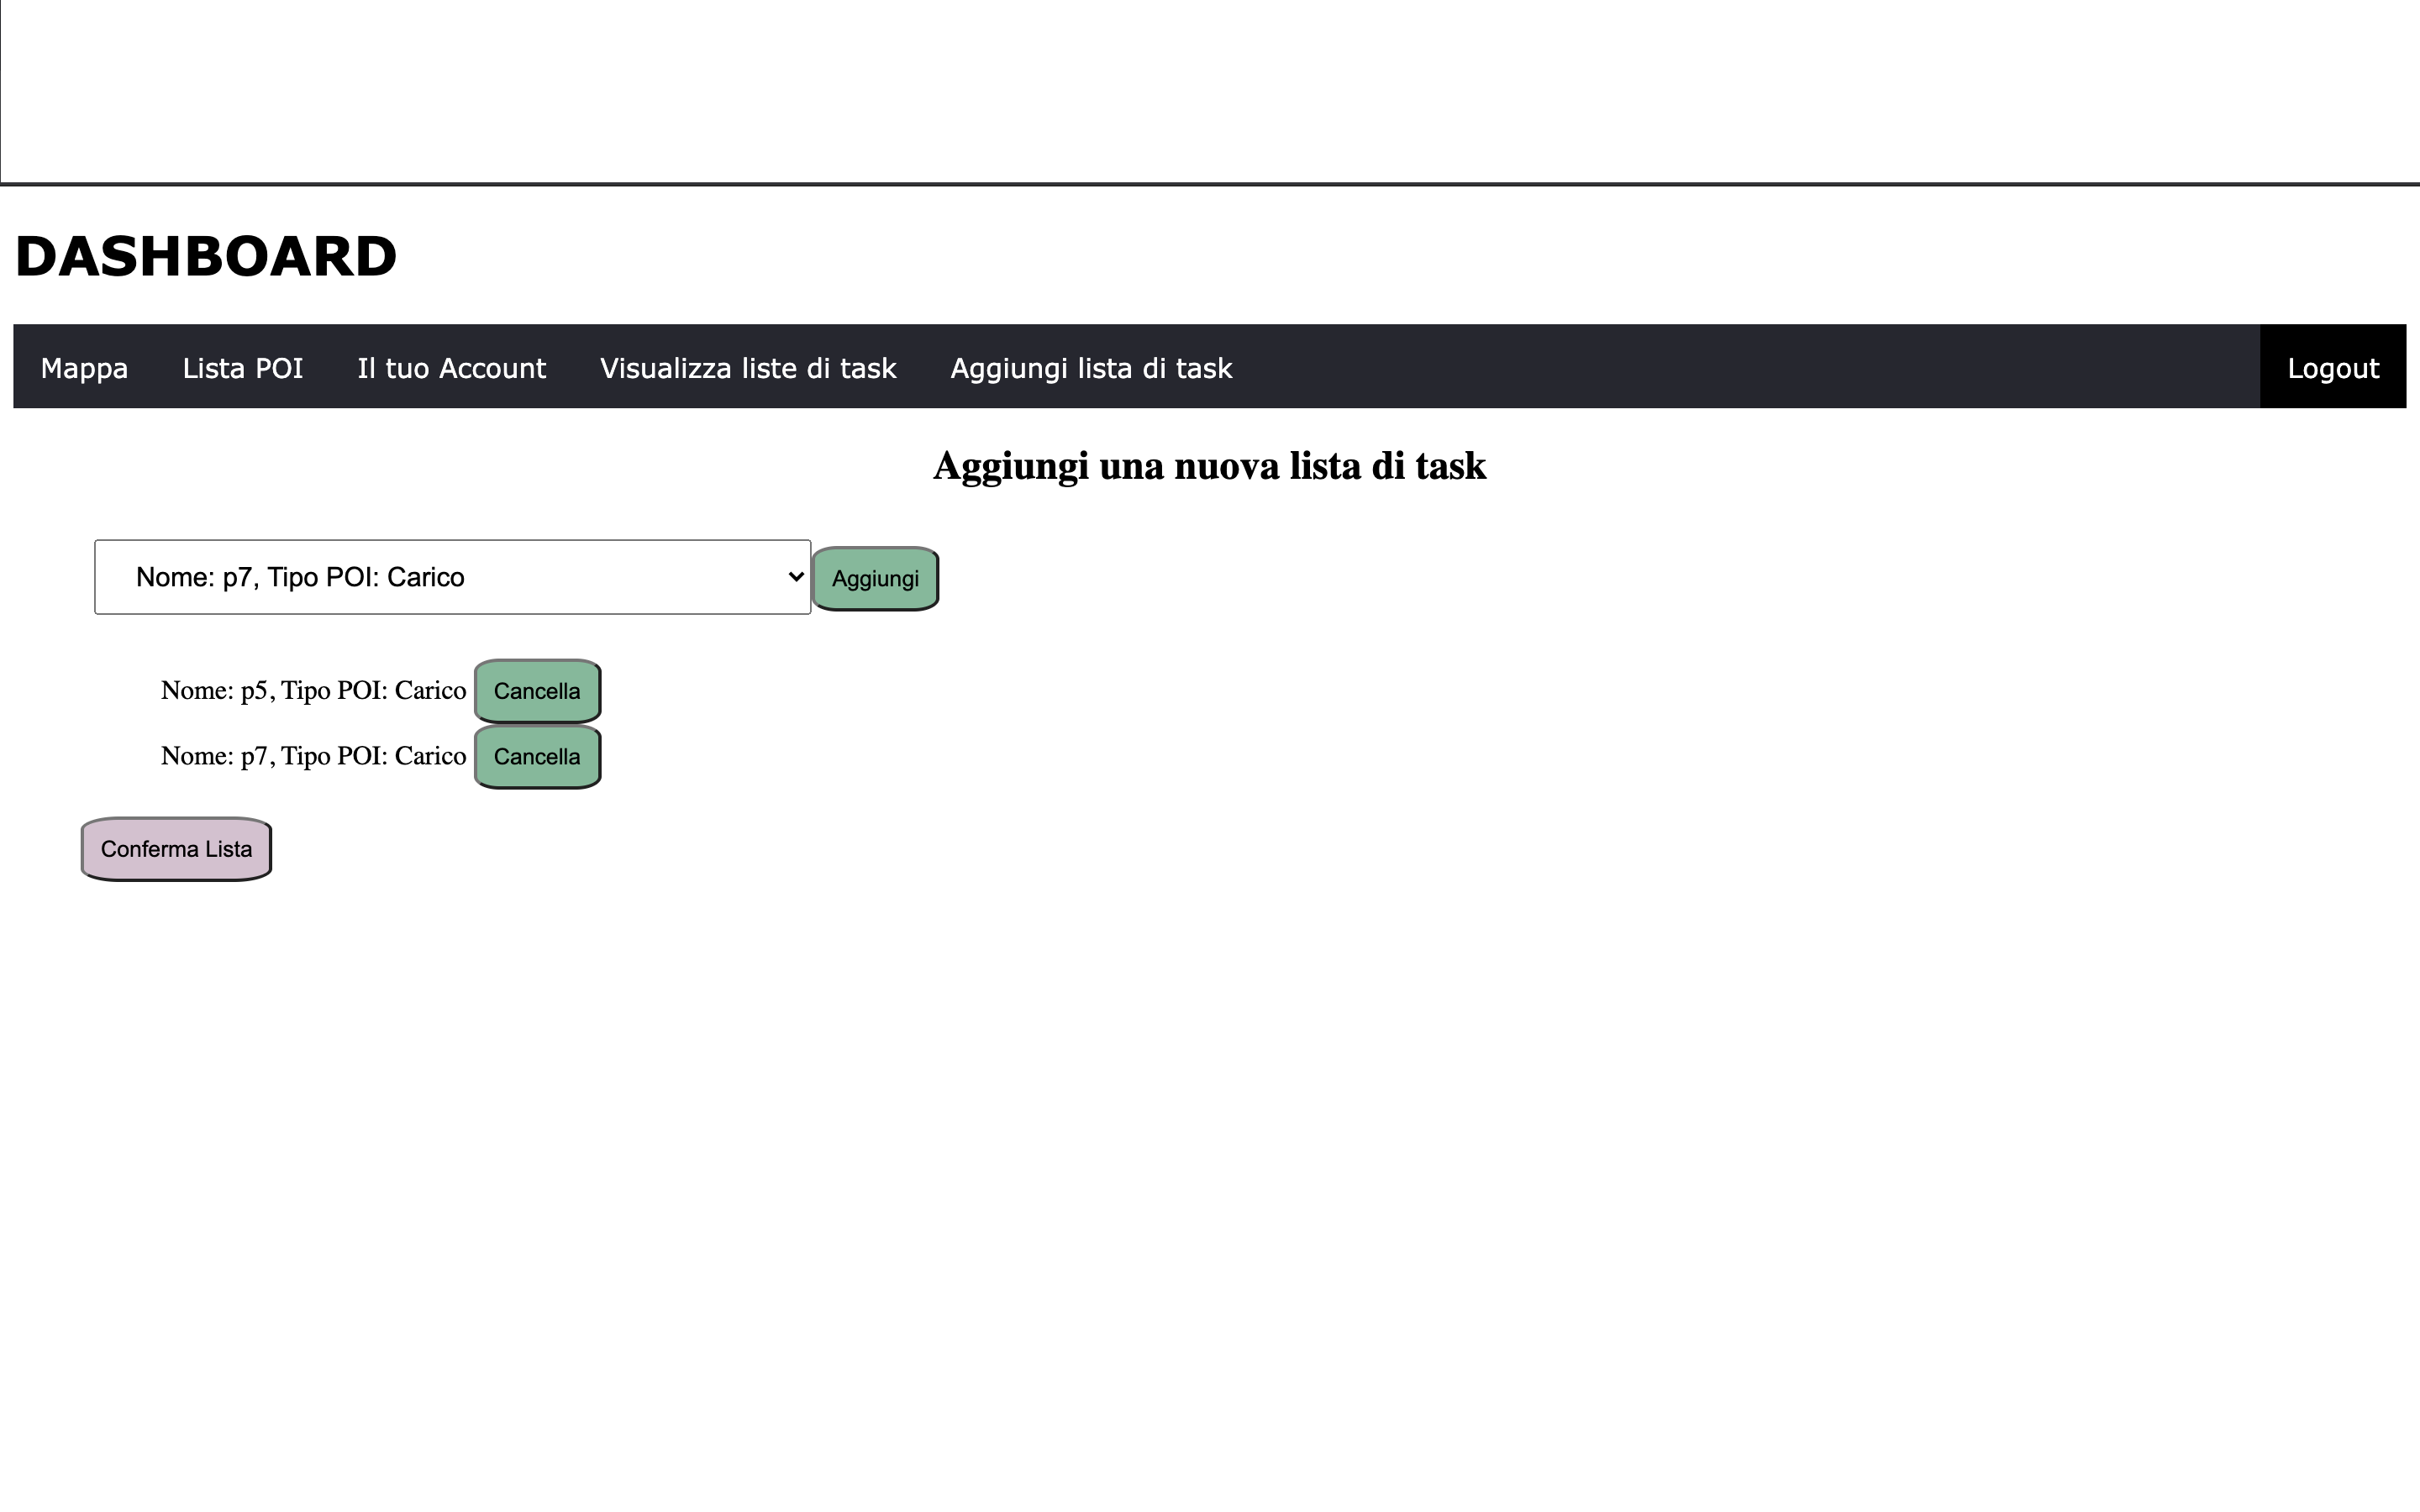
\includegraphics[scale=0.12]{res/images/newtask_manager.png}
    \caption{Schermata guida automatica dell'unità}
\end{figure}

\subsubsection{Eliminare una lista di task non ancora assegnata}
\begin{itemize}
    \item Premere sul pulsante "Elimina lista di task"
    \item viene visualizzata la lista di task non ancora assegnate;
    \item tramite il pulsante "Elimina" di fianco ad ogni lista è possibile eliminare la lista;
    \item per tornare alla pagina iniziale serve premere sul pulsante "Chiudi".
\end{itemize}
\begin{figure}[H]
    \centering
    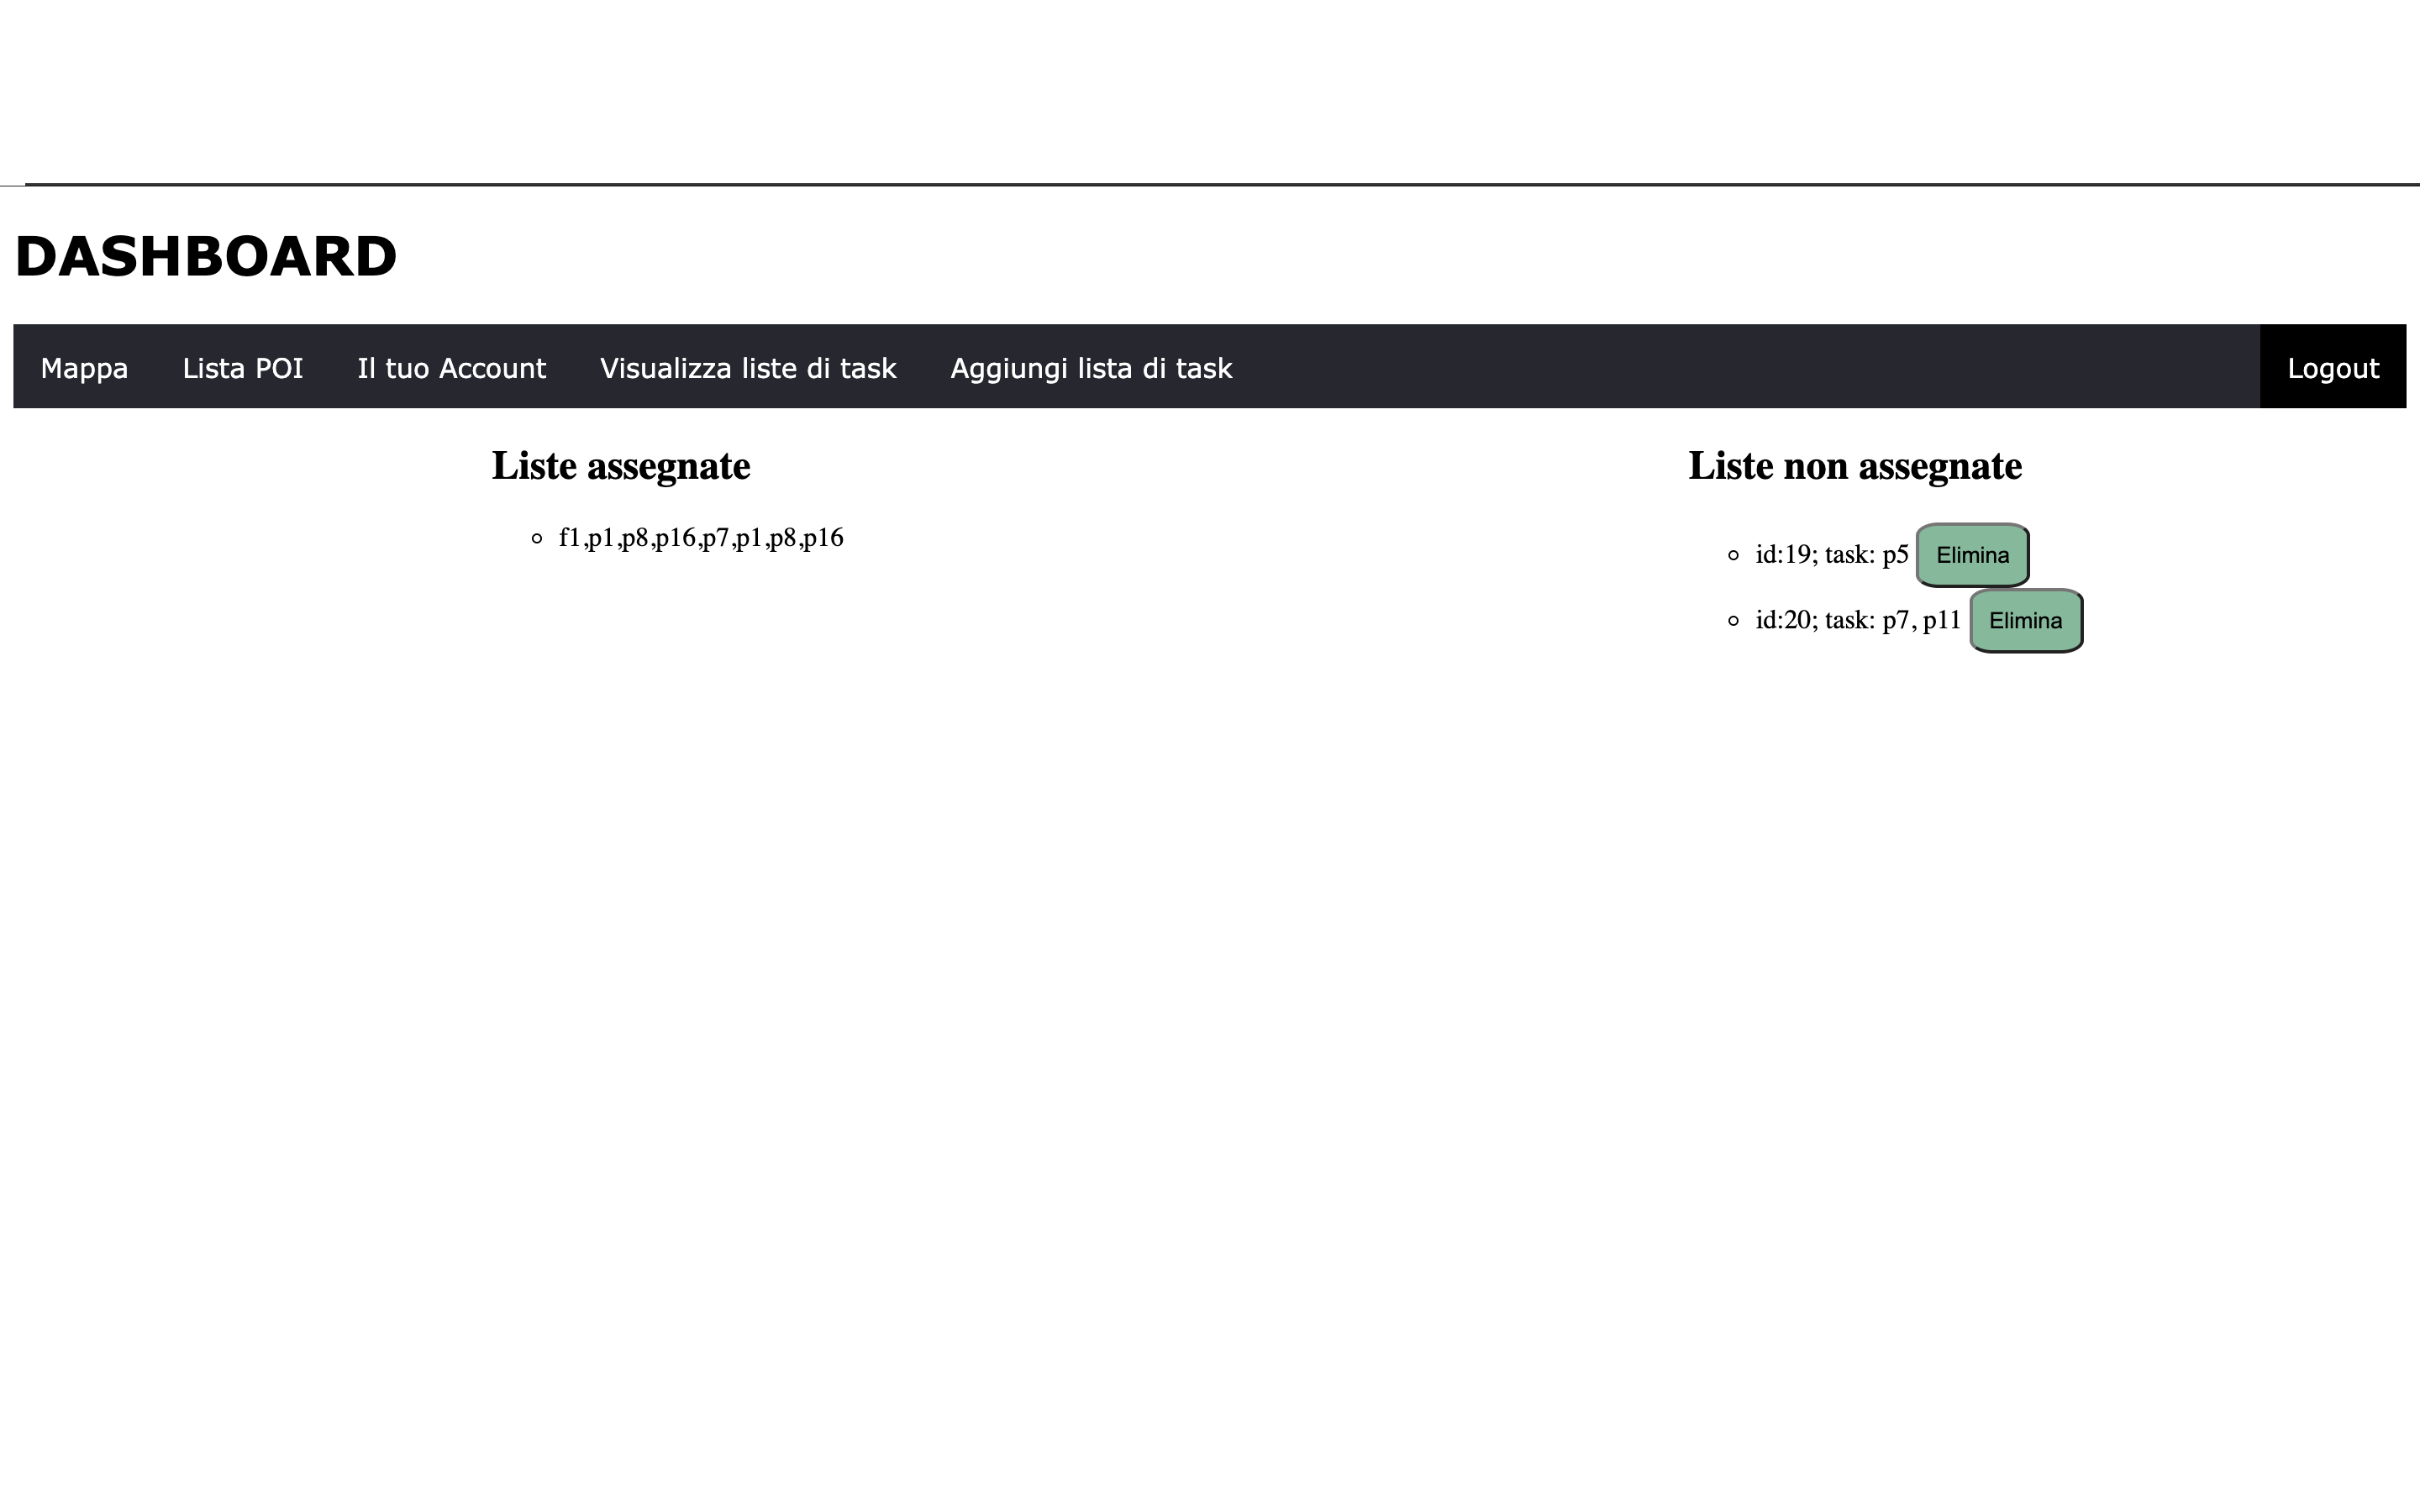
\includegraphics[scale=0.12]{res/images/task_manager.png}
    \caption{Schermata guida automatica dell'unità}
\end{figure}
	\pagebreak
	\section{Istruzione utilizzo utente operatore}
La seguente sezione fornirà indicazioni utili per il corretto utilizzo del software nel caso l'utente interessato sia l'operatore che deve guidare l'unità.

\subsection{Guida automatica dell'unità}
\begin{itemize}
    \item Premere sul pulsante "Start" per iniziare il movimento del muletto verso il primo POI della lista;
    \item i movimenti effettuati sono visualizzati nella mappa e nelle frecce.
    
\end{itemize}
\begin{figure}[H]
    \centering
    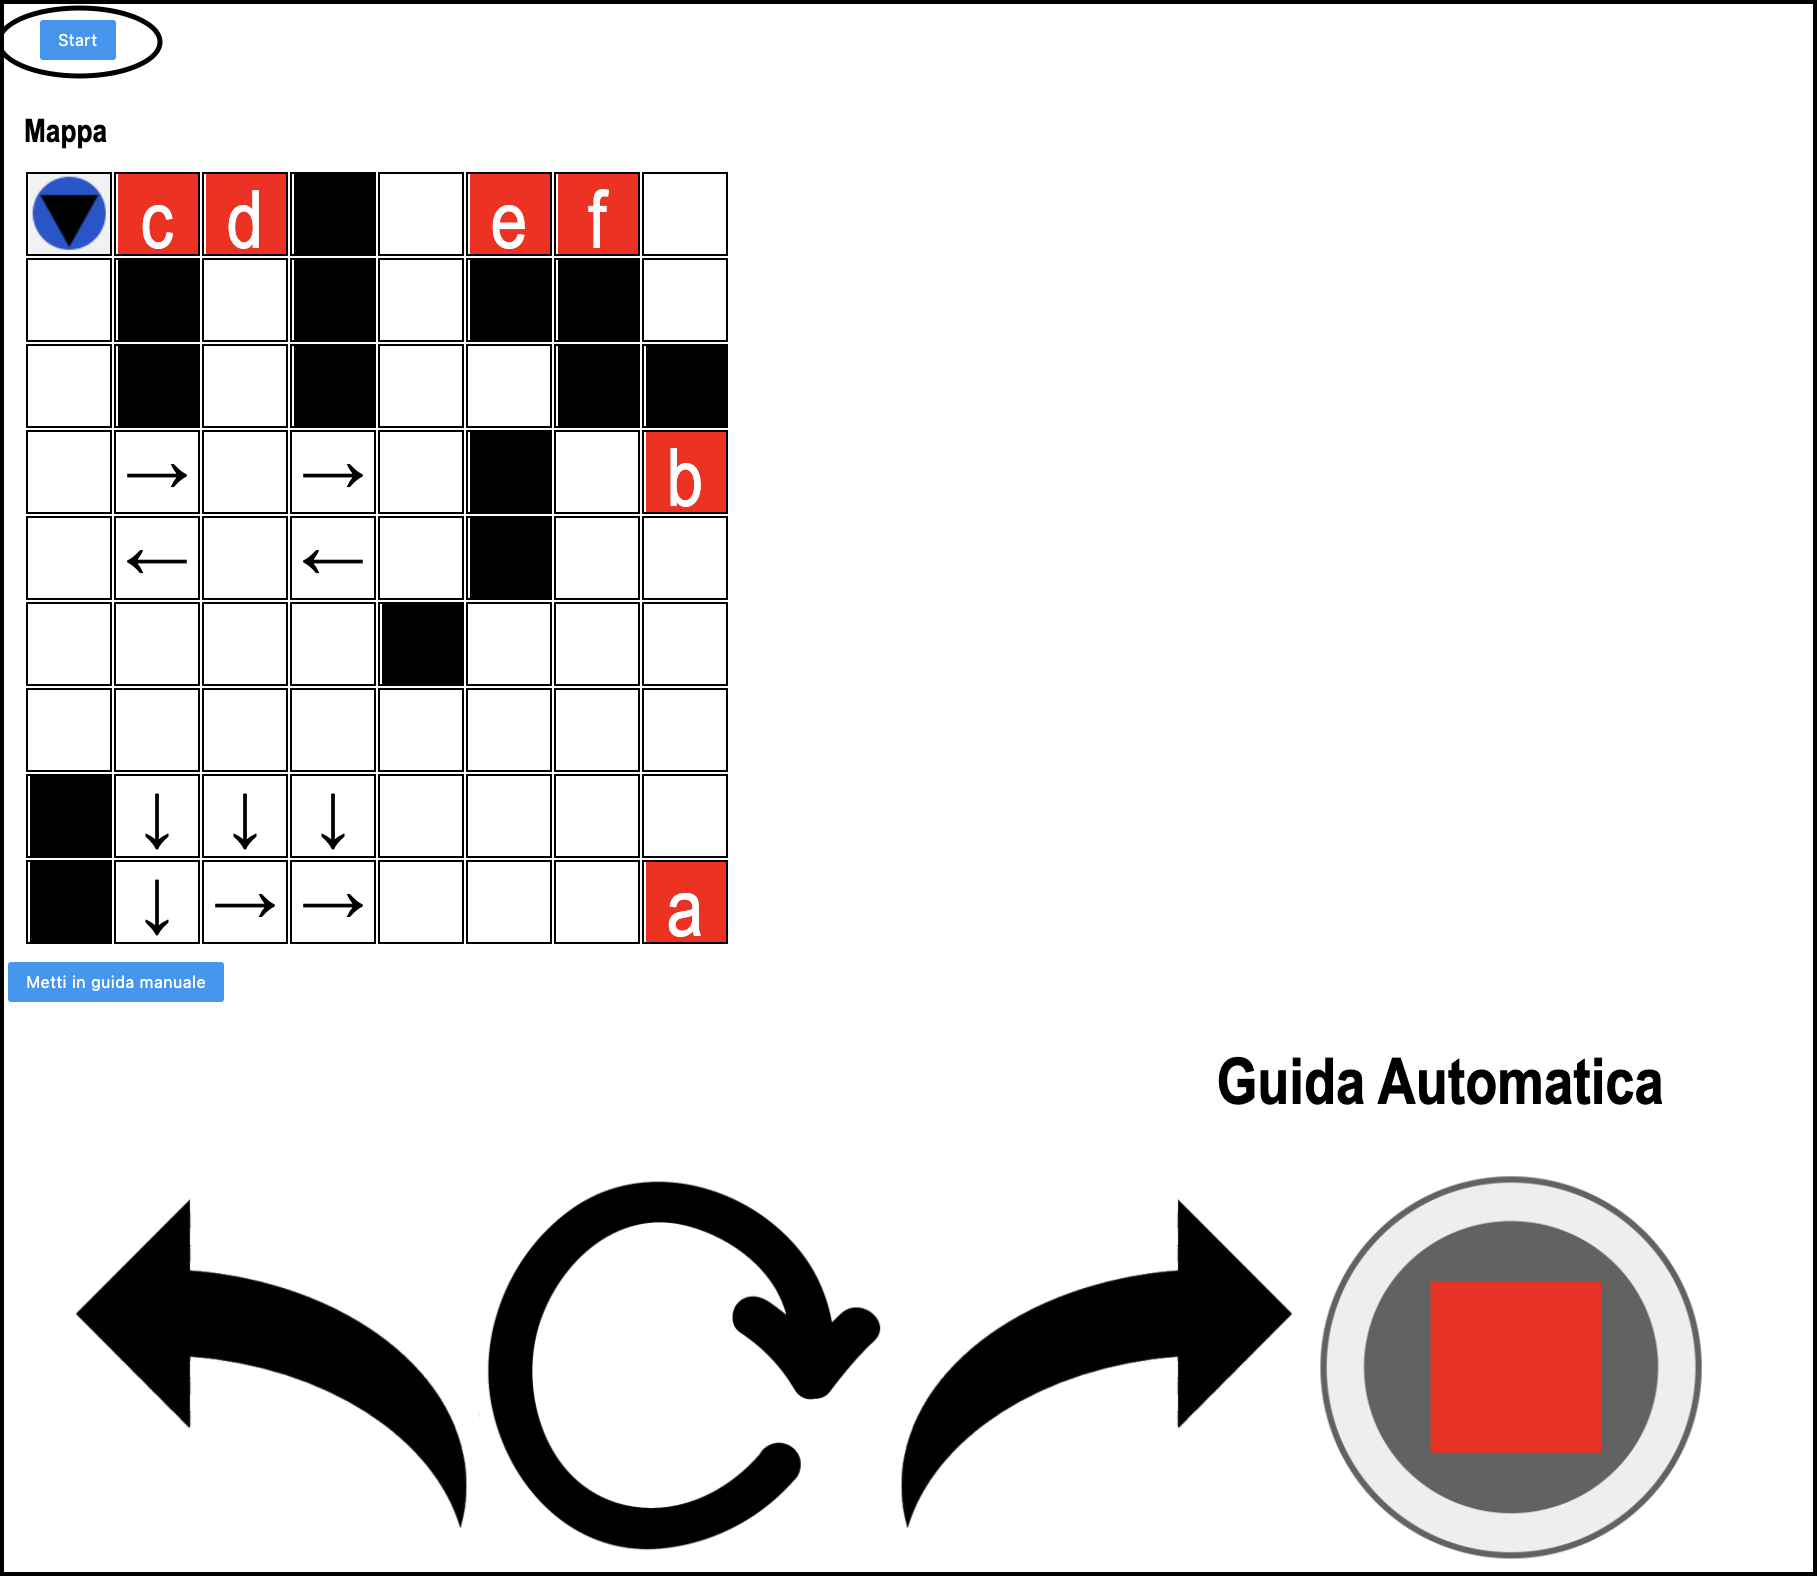
\includegraphics[scale=0.45]{res/images/forklift_start.png}
    \caption{Schermata guida automatica dell'unità}
\end{figure}
\pagebreak
\subsection{Passaggio a guida manuale/automatica}
\begin{itemize}
    \item Premere sul pulsante "Cambio guida";
    \item i comandi verranno cambiati in base allo stato di guida;
\end{itemize}
\begin{figure}[H]
    \centering
    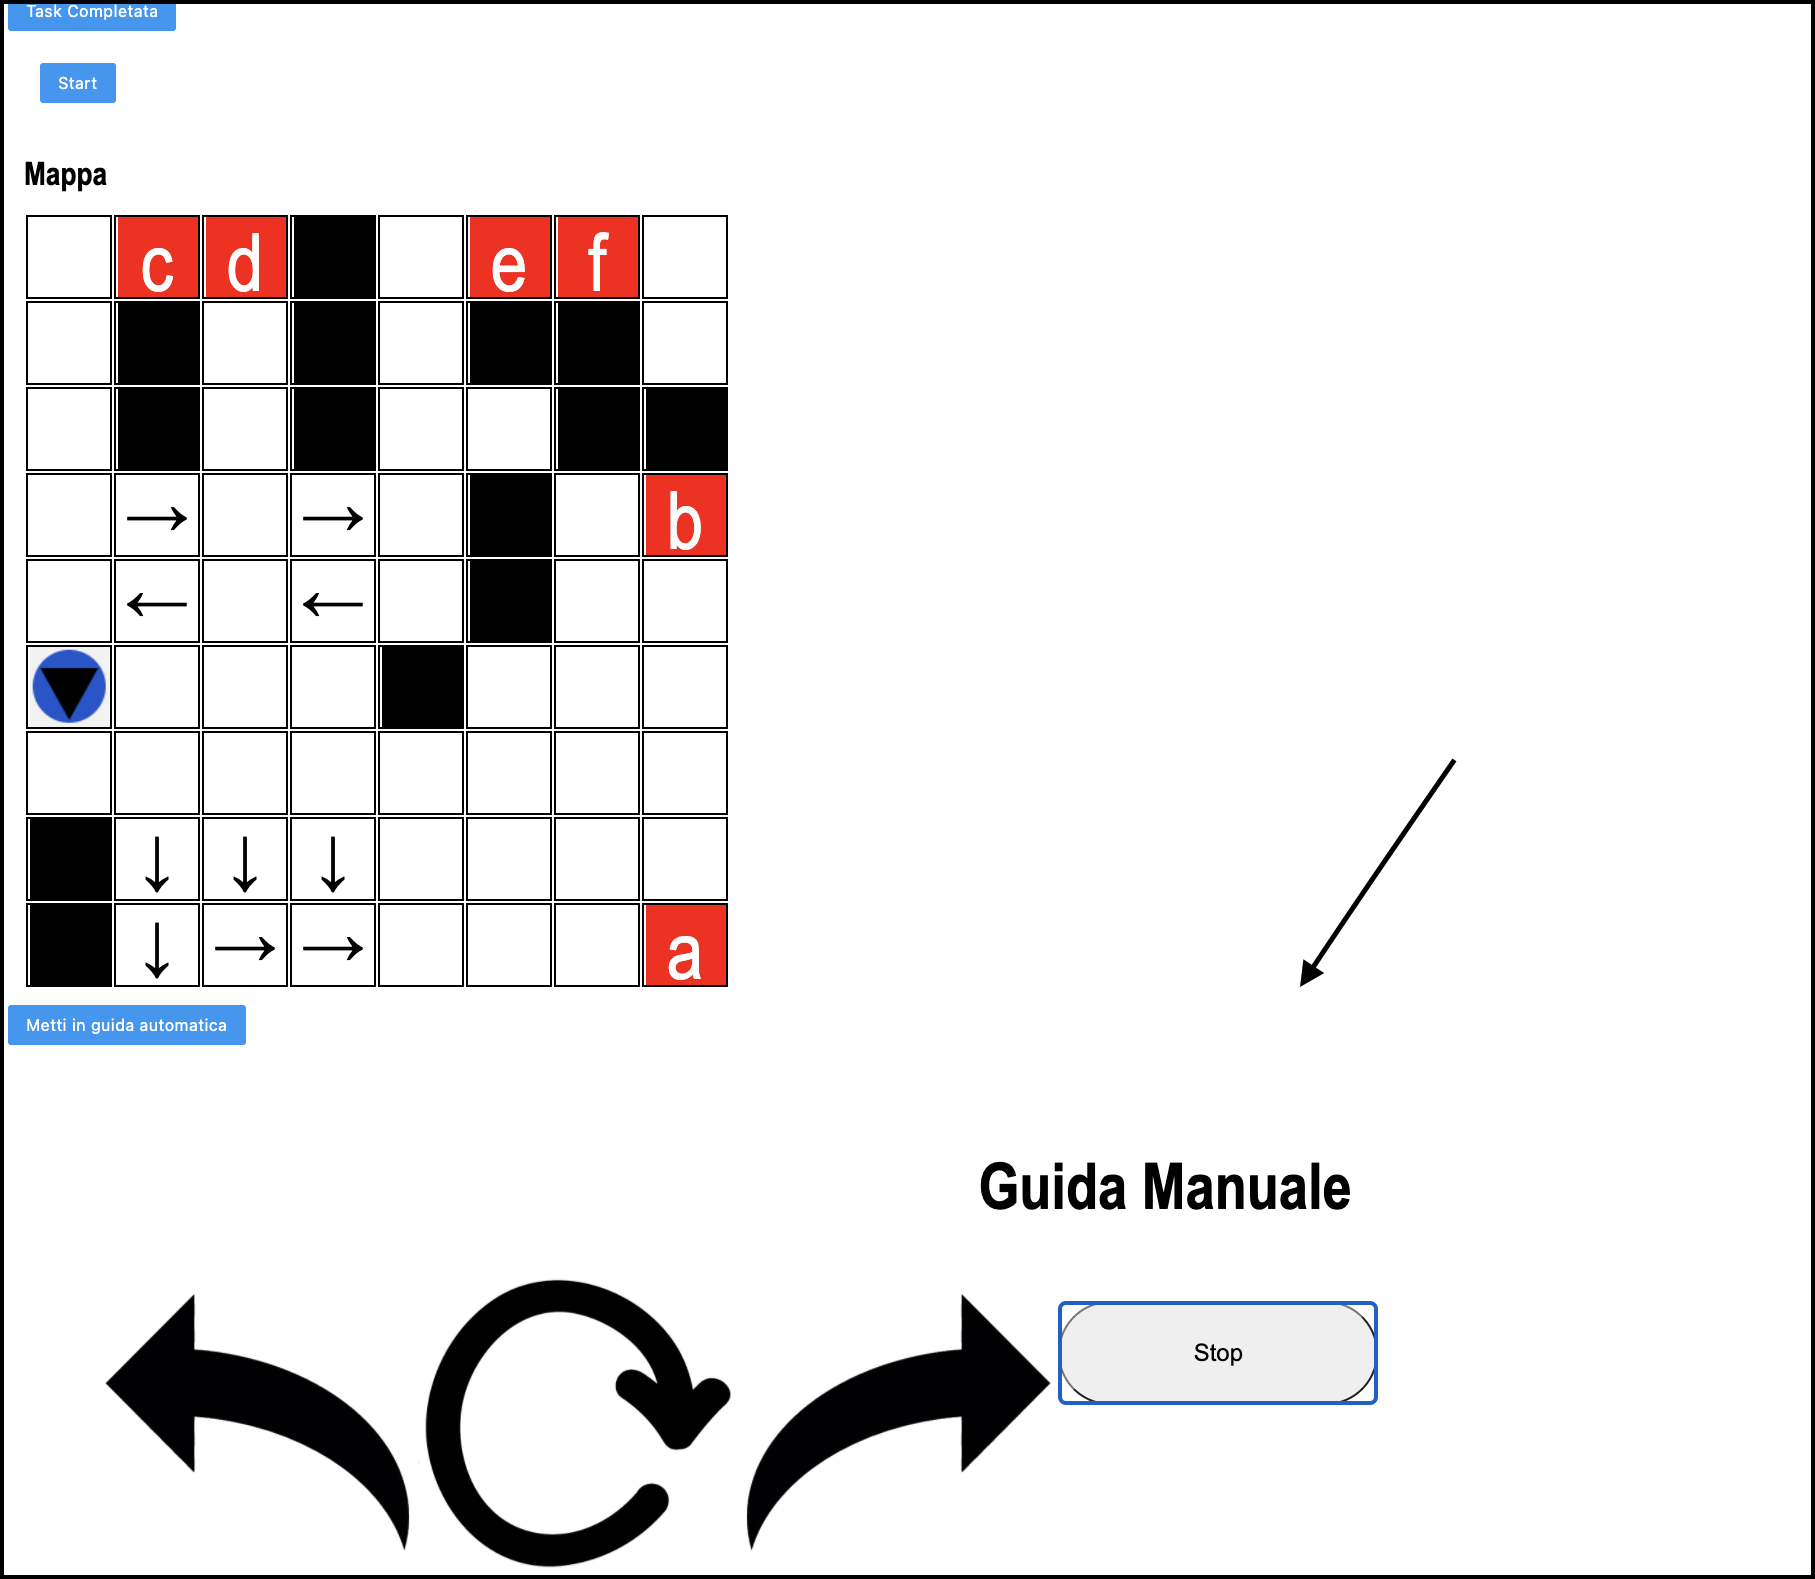
\includegraphics[scale=0.45]{res/images/forklift_guidamanuale.png}
    \caption{Schermata passaggio a guida manuale}
\end{figure}
\begin{figure}[H]
    \centering
    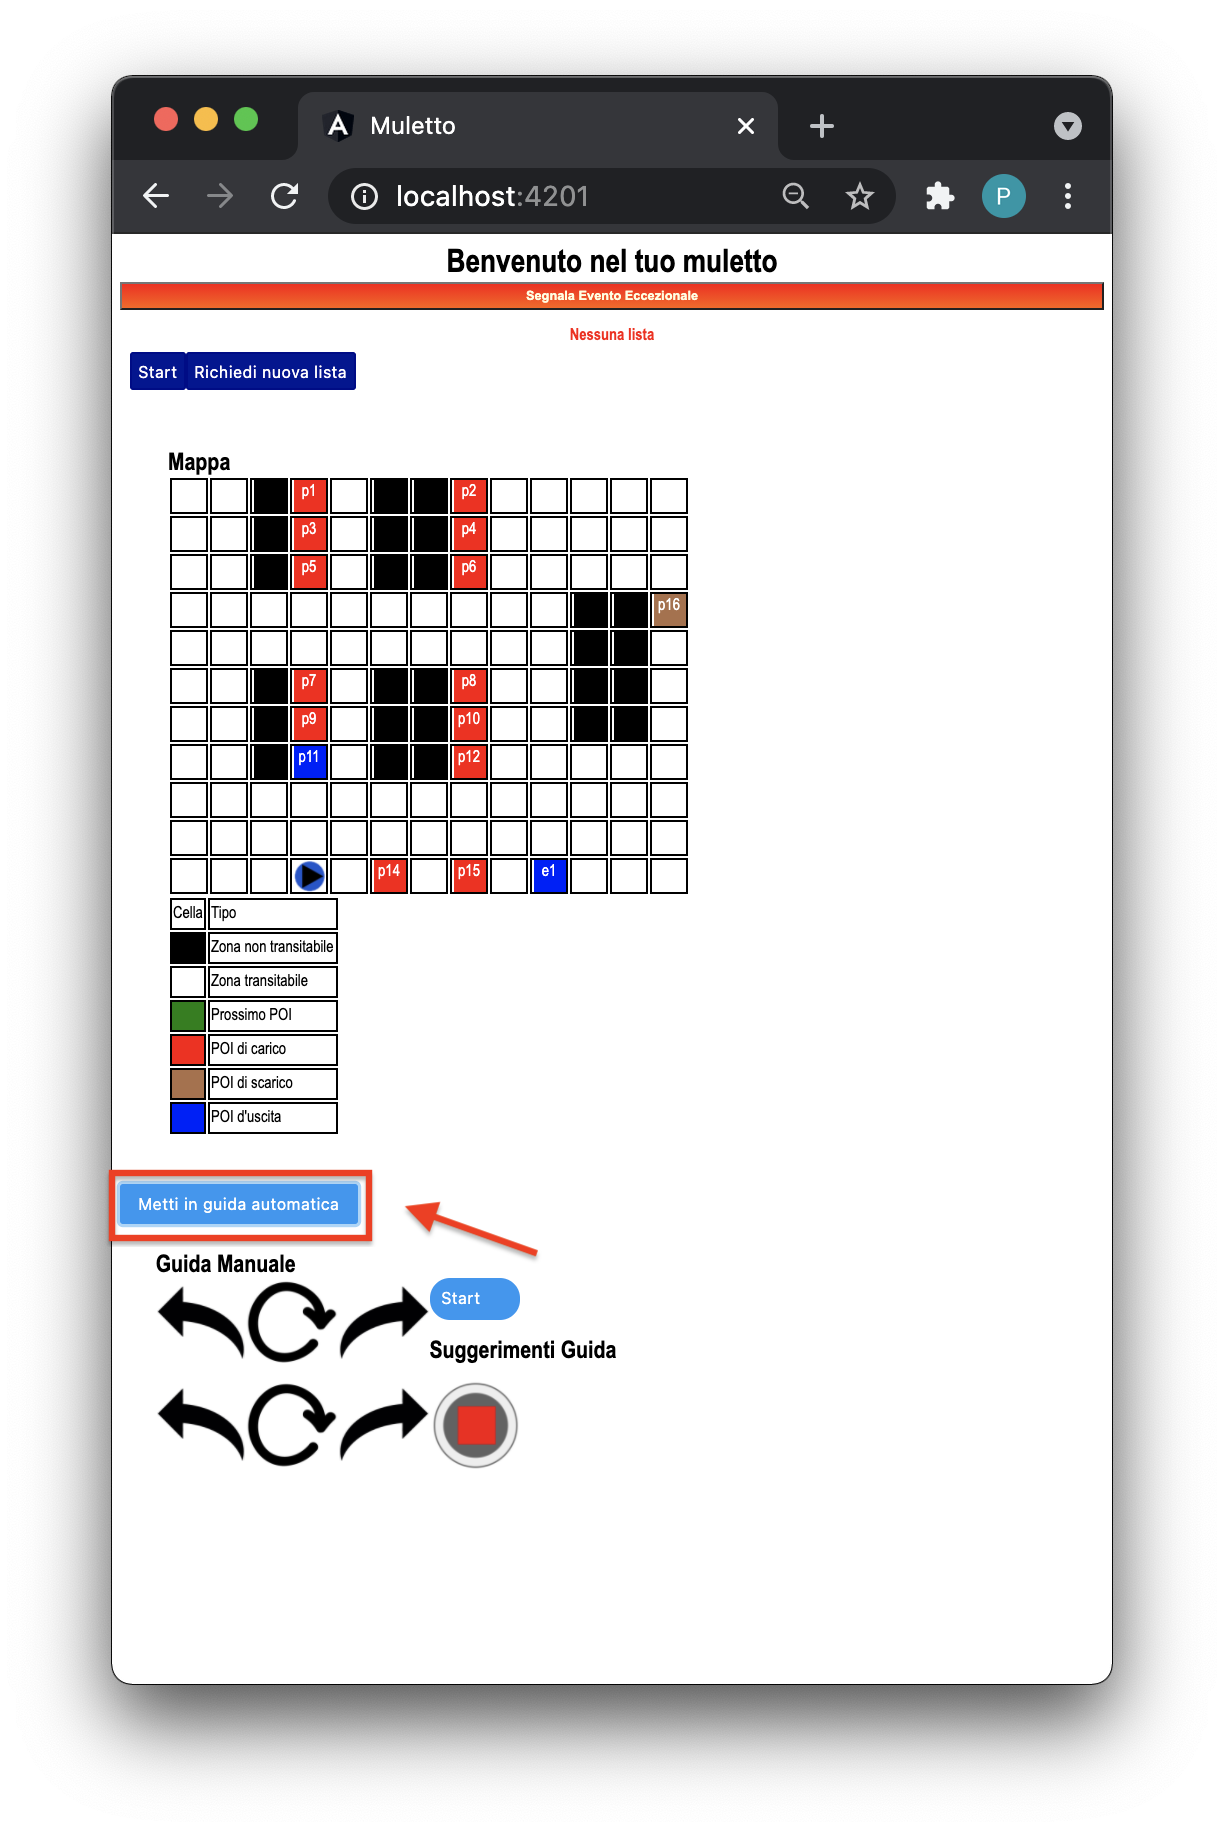
\includegraphics[scale=0.45]{res/images/forklift_cambioautomatica.png}
    \caption{Schermata passaggio a guida automatica}
\end{figure}
\pagebreak

\subsection{Guida manuale dell'unità}
\begin{itemize}
    \item Premere sul pulsante "Metti in guida manuale";
    \begin{figure}[H]
        \centering
          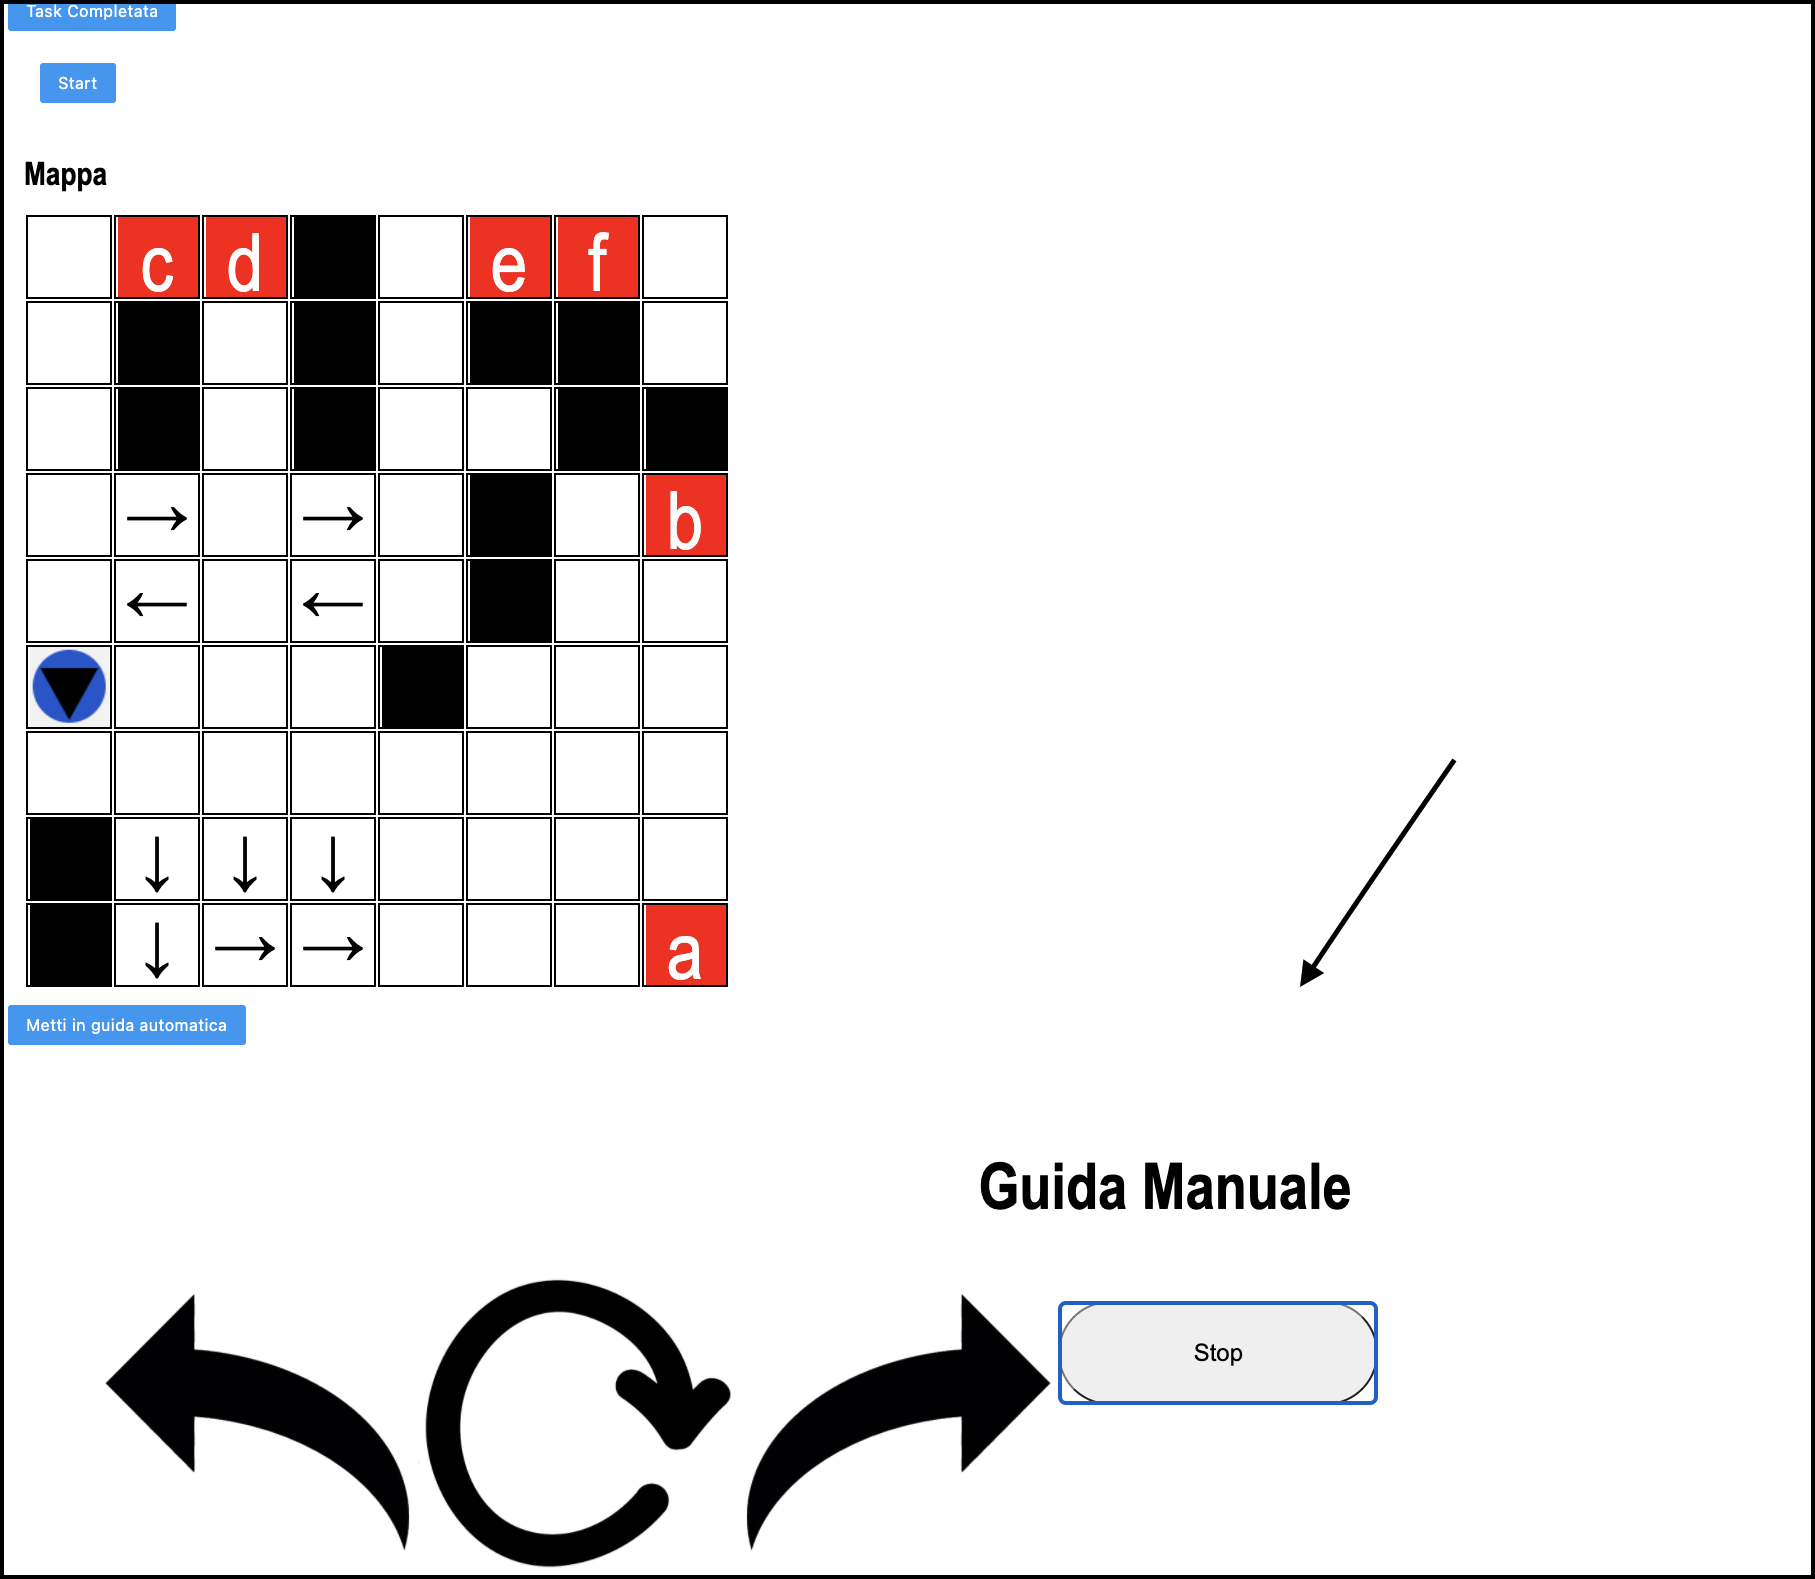
\includegraphics[scale=0.45]{res/images/forklift_guidamanuale.png}
          \caption{Schermata guida manuale dell'unità}
    \end{figure}
    \item tramite il pulsante "Start" viene avviato il movimento del muletto verso la direzione in cui è rivolto;
    \begin{figure}[H]
        \centering
          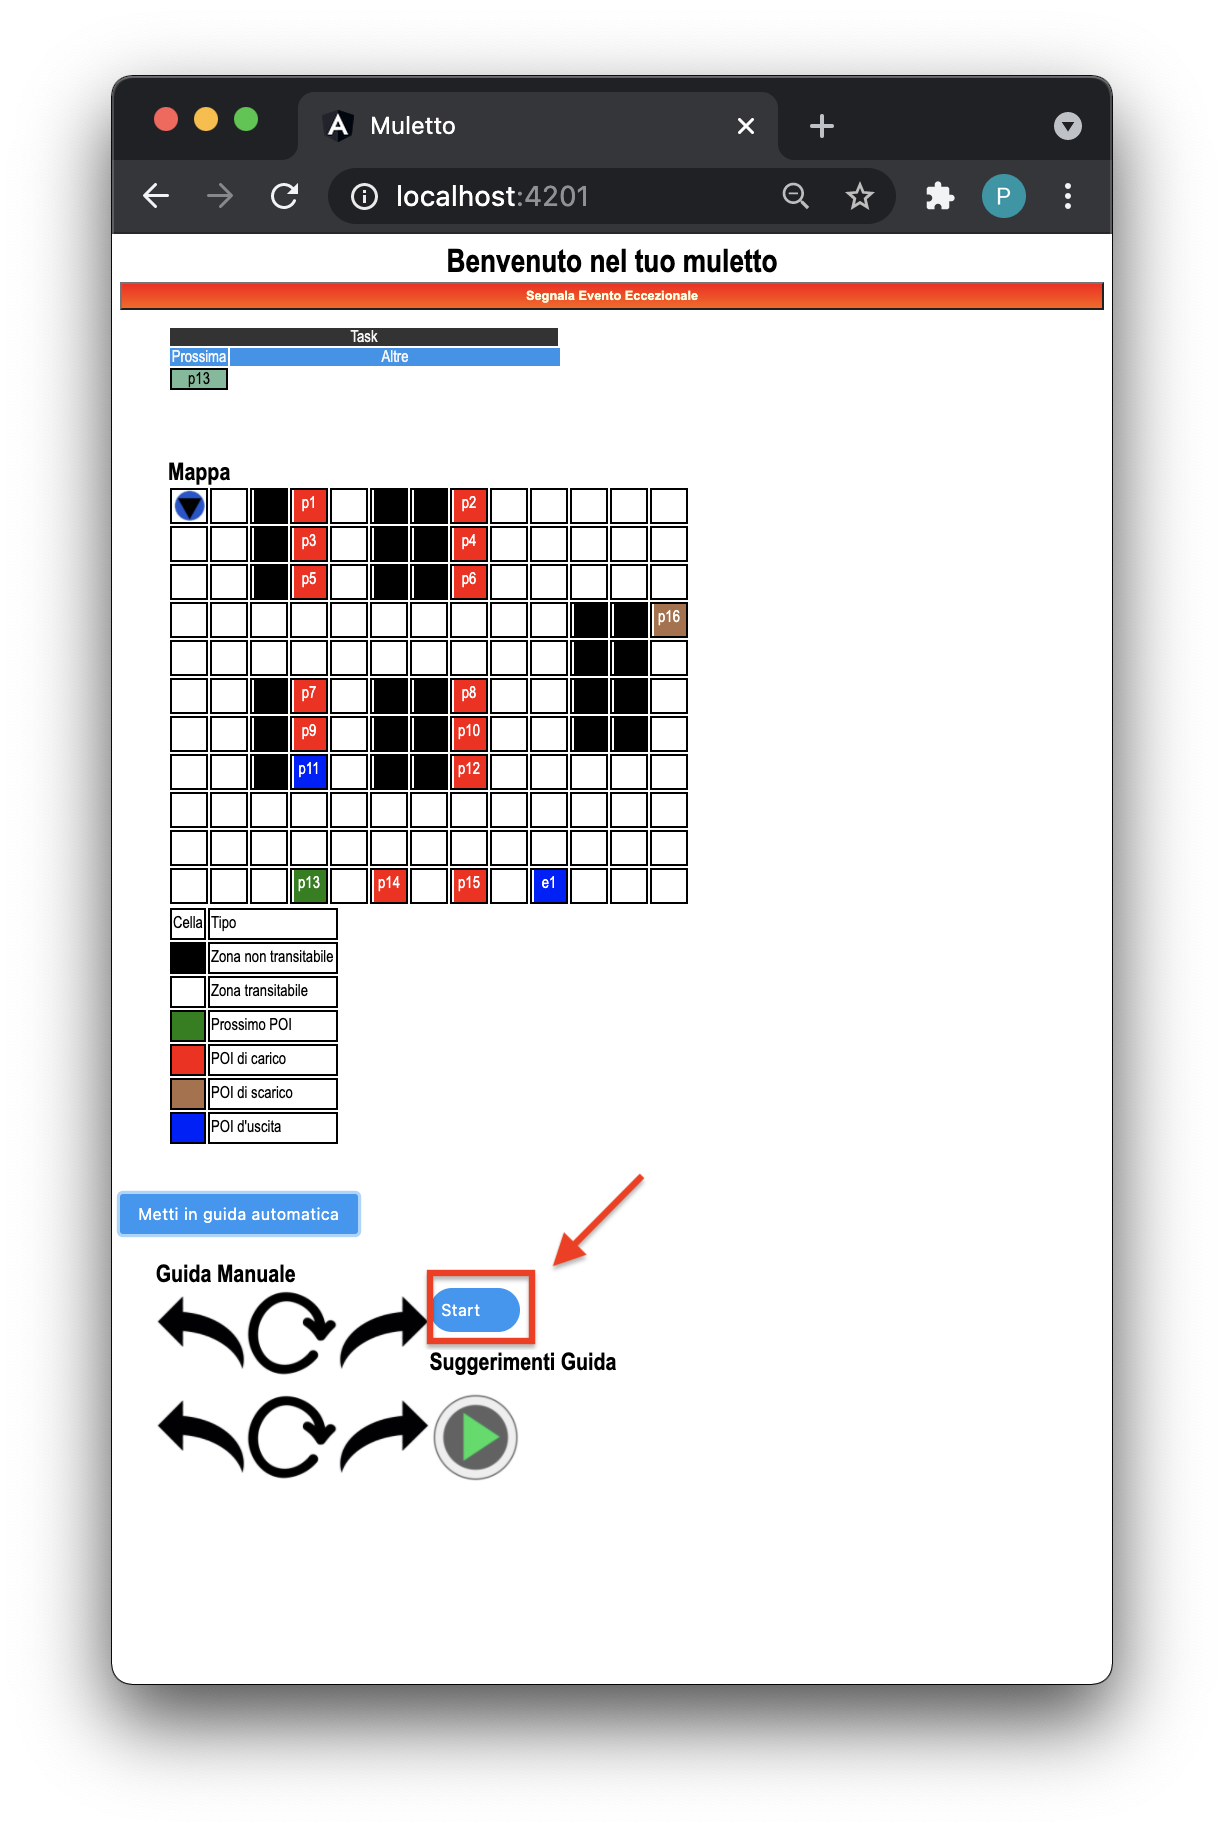
\includegraphics[scale=0.45]{res/images/guidamanuale.png}
          \caption{Schermata guida manuale dell'unità}
    \end{figure}
    \item premendo le frecce il muletto ruota di 90 gradi o 180 gradi;
    \begin{figure}[H]
        \centering
          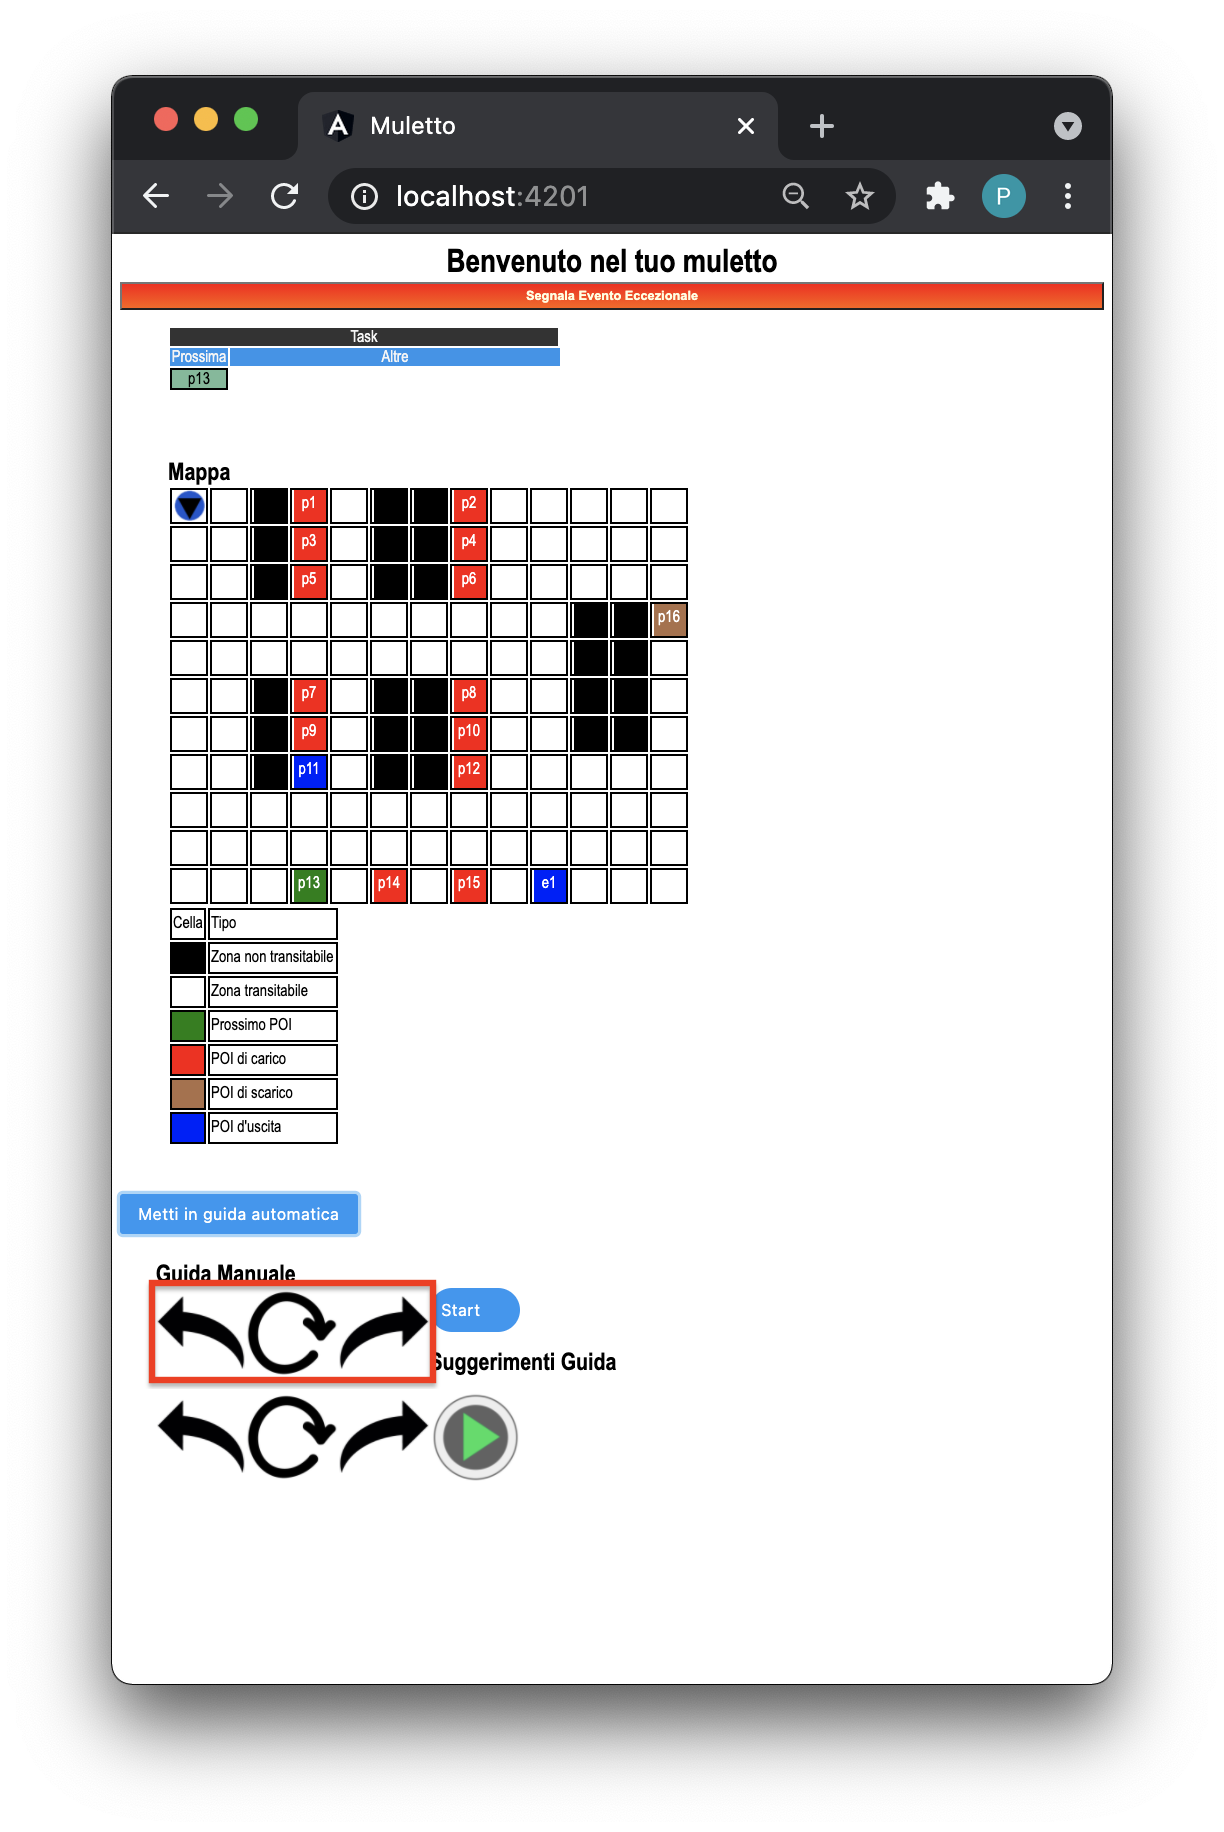
\includegraphics[scale=0.45]{res/images/guidamanuale1.png}
          \caption{Schermata guida manuale dell'unità}
    \end{figure}
    \item premendo il pulsante "Stop" viene fermato il movimento;
    \begin{figure}[H]
        \centering
          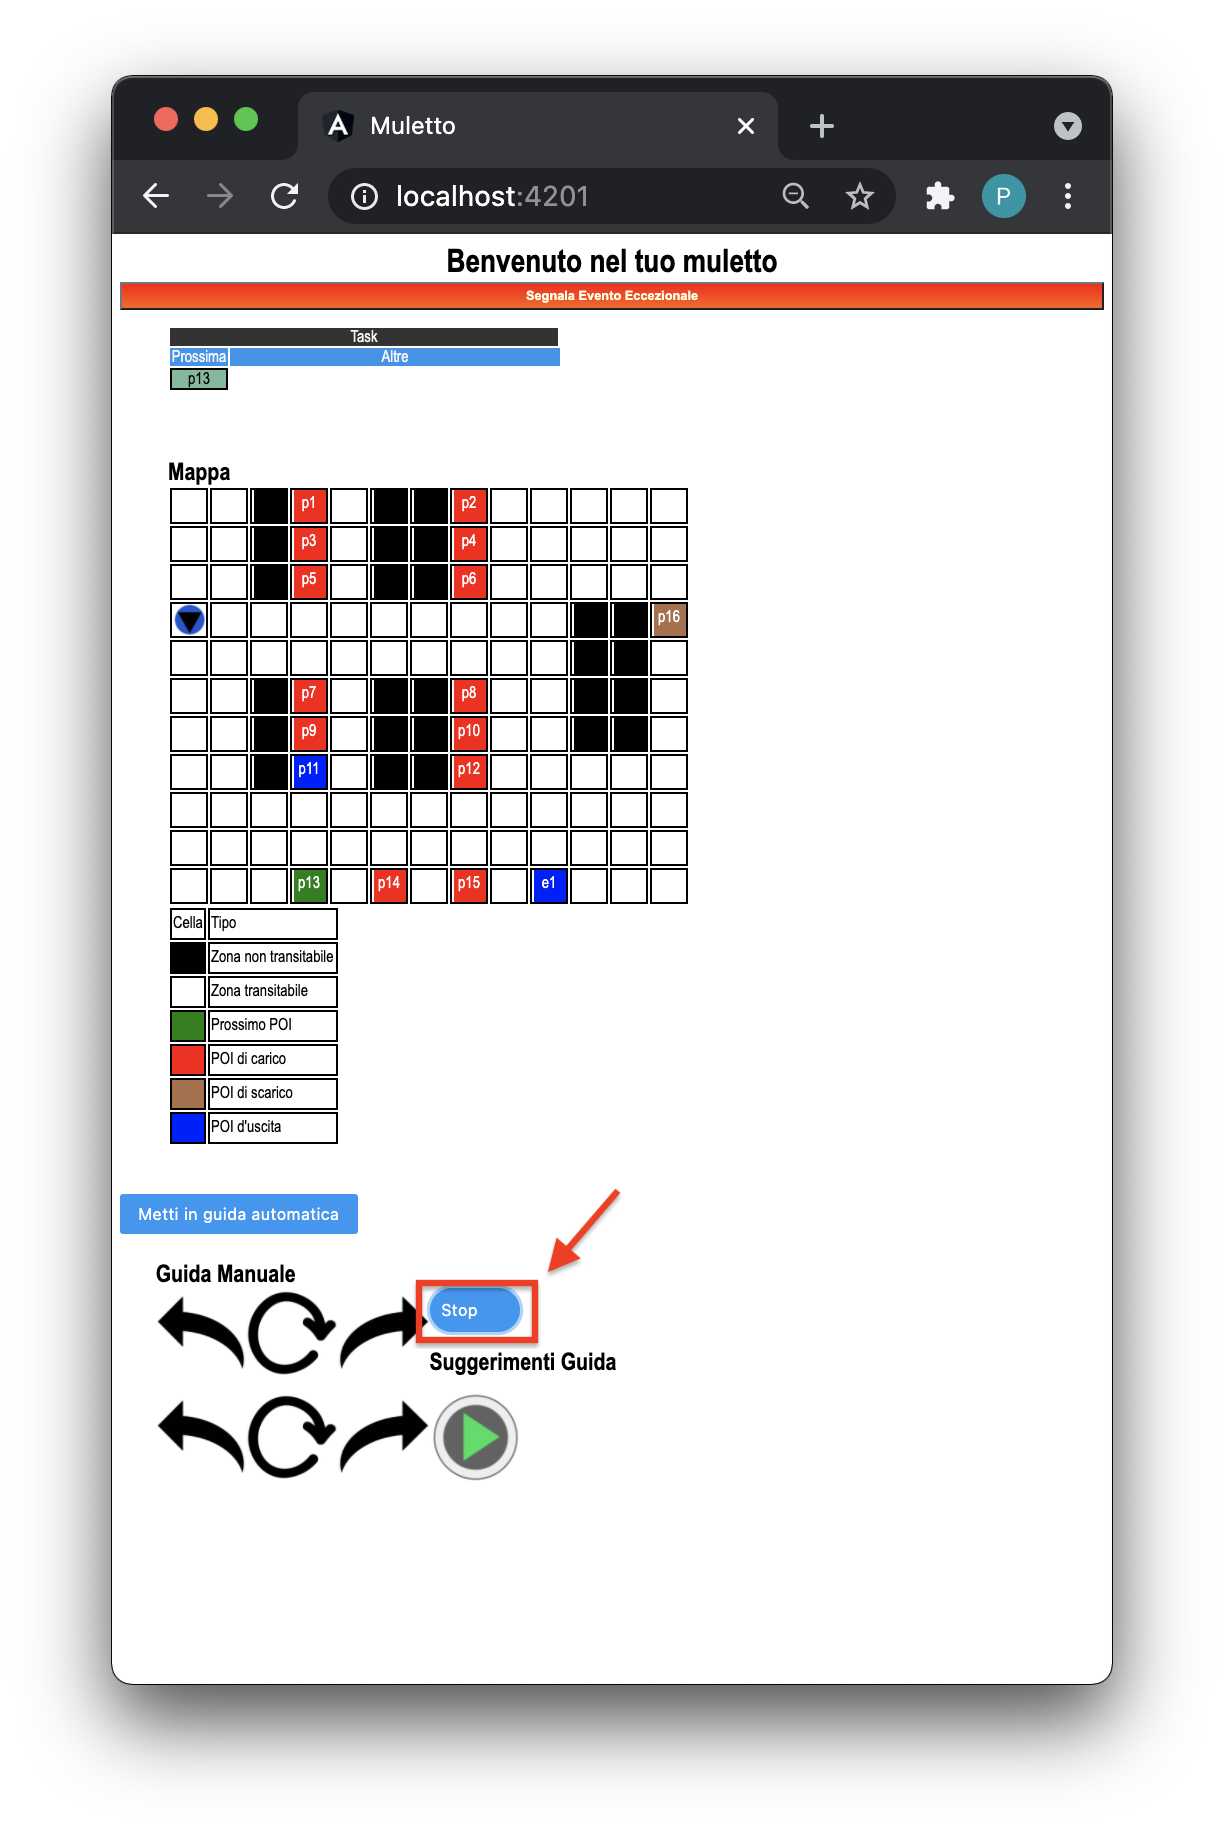
\includegraphics[scale=0.45]{res/images/guidamanuale_stop.png}
          \caption{Schermata guida manuale dell'unità}
    \end{figure}
    \item sotto sono visualizzati i suggerimenti del percorso più breve per il raggiungimento del POI interessato.
    \begin{figure}[H]
        \centering
          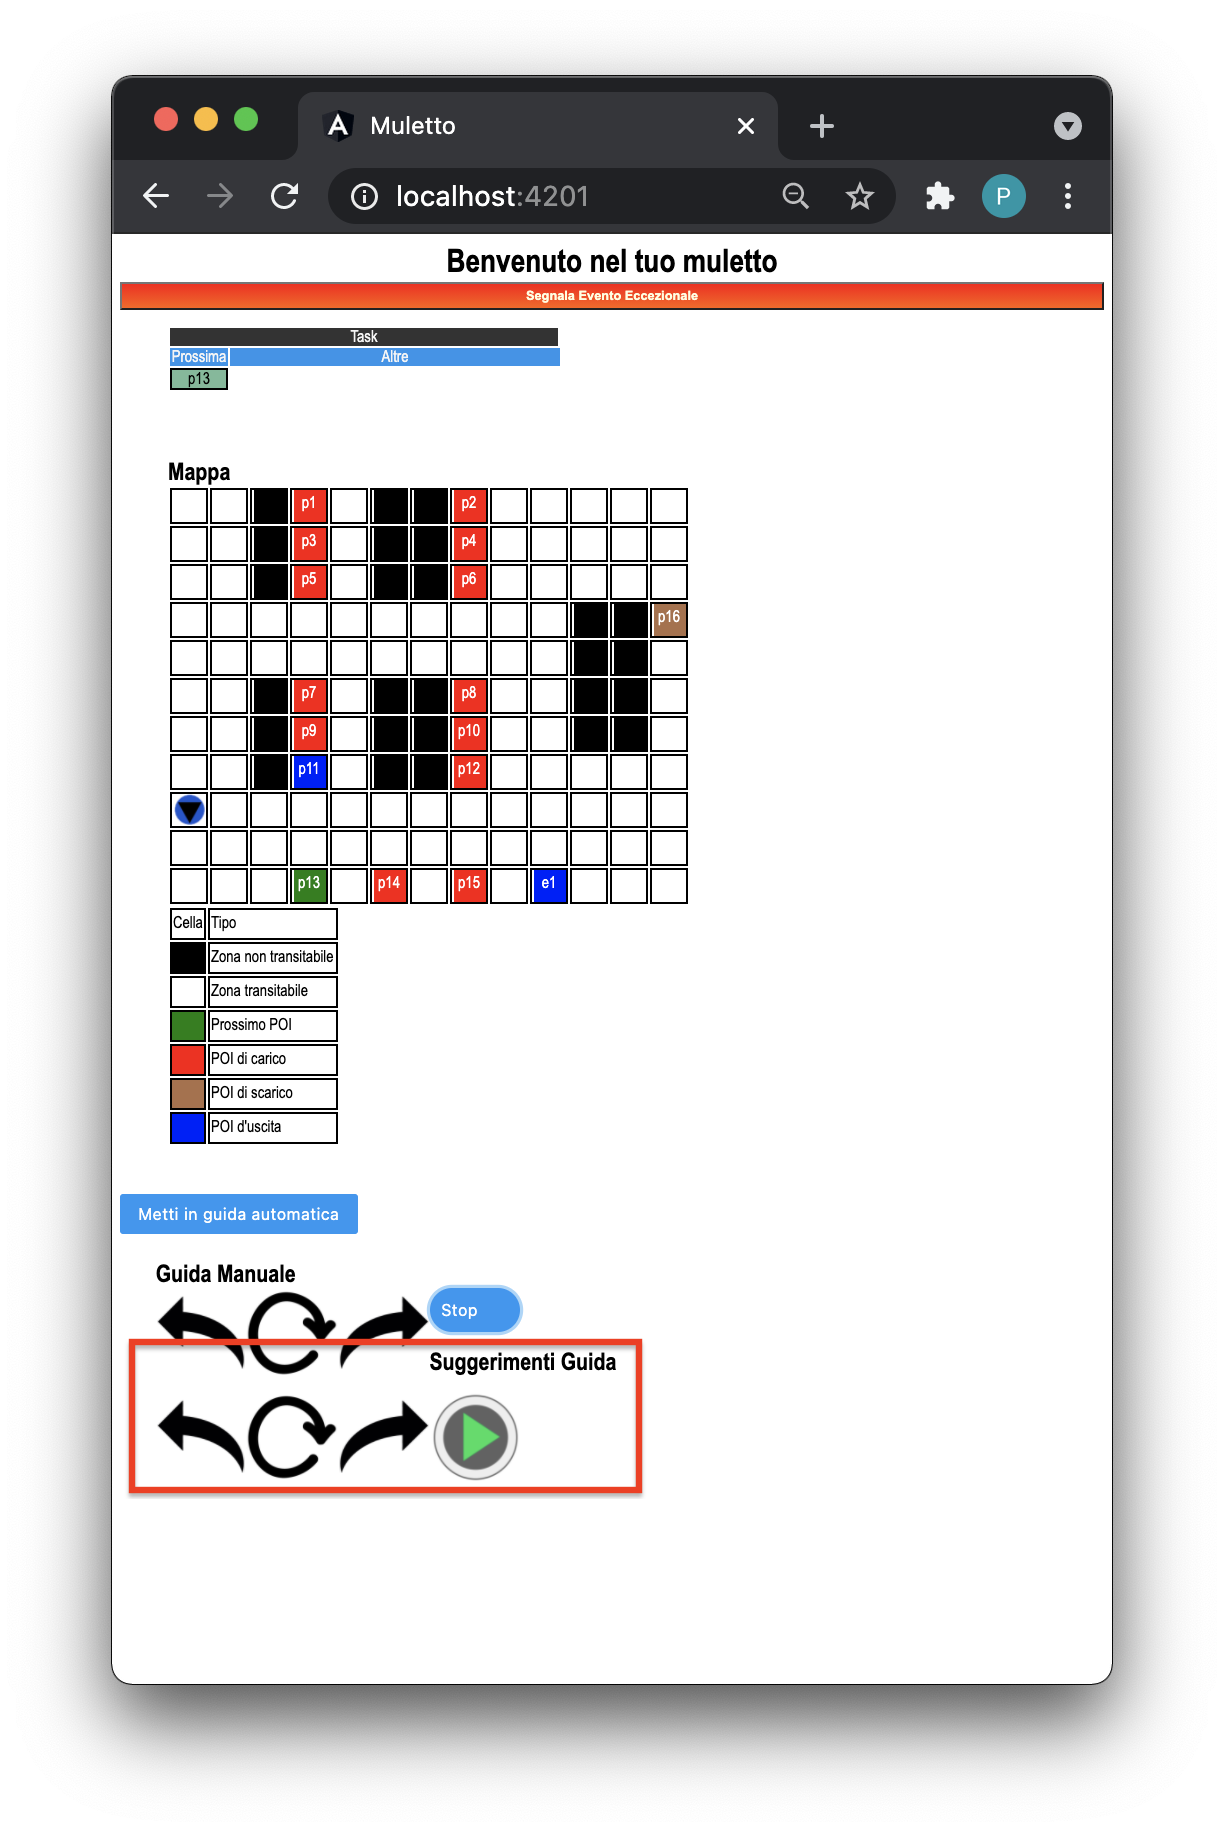
\includegraphics[scale=0.45]{res/images/suggerimenti.png}
          \caption{Schermata guida manuale dell'unità}
    \end{figure}
\end{itemize}

\subsection{Completamento task}
\begin{itemize}
    \item Una volta raggiunto il POI, l'unità si ferma e viene visualizzato un pulsante "Task completata";
    \item premere su esso per notificare lo scarico delle merci e per continuare il proprio percorso;
    \begin{figure}[H]
        \centering
        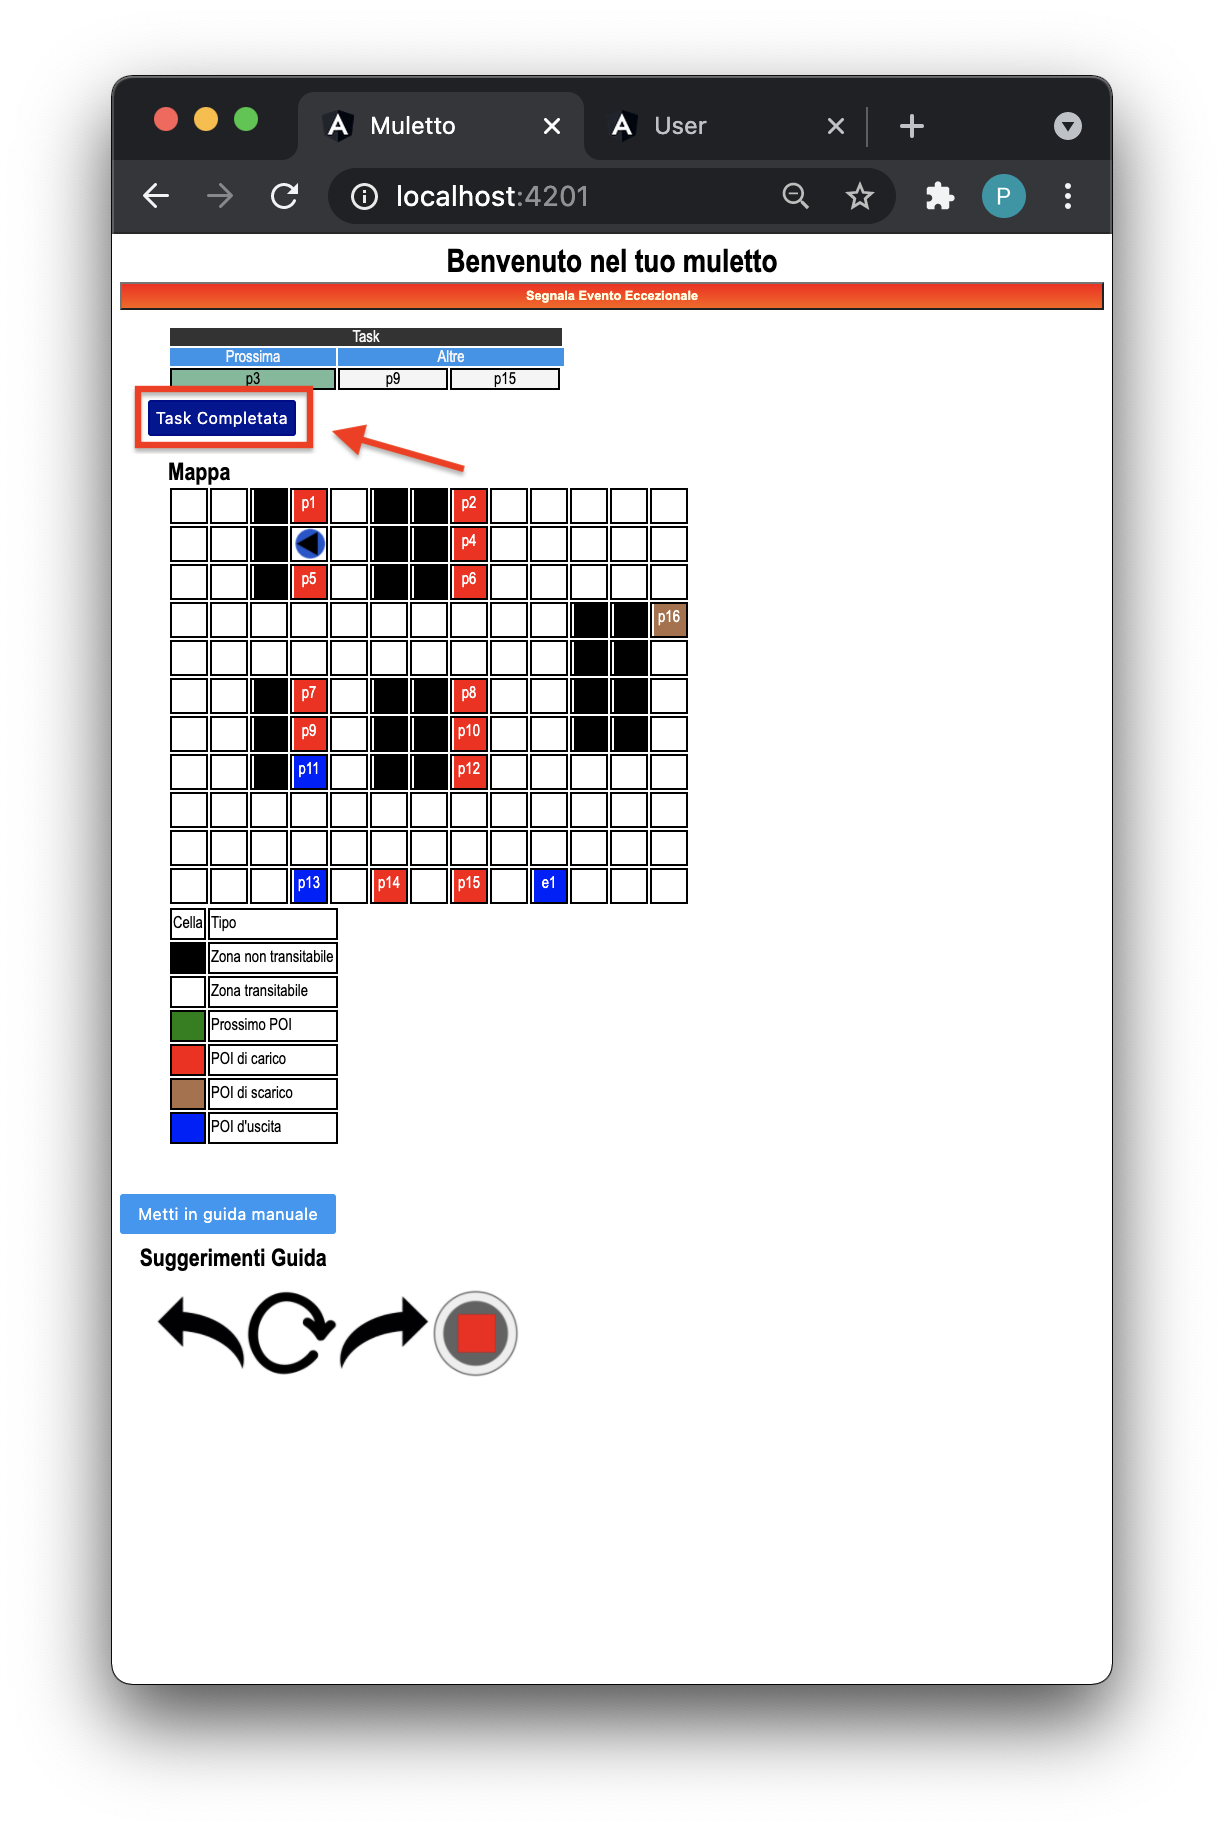
\includegraphics[scale=0.45]{res/images/forklift_taskcompletata.png}
    \end{figure}
    \item verrà quindi evidenziato in verde il prossimo POI da raggiungere e l'unità si recherà in esso se in guida automatica.
    \item \begin{figure}[H]
        \centering
        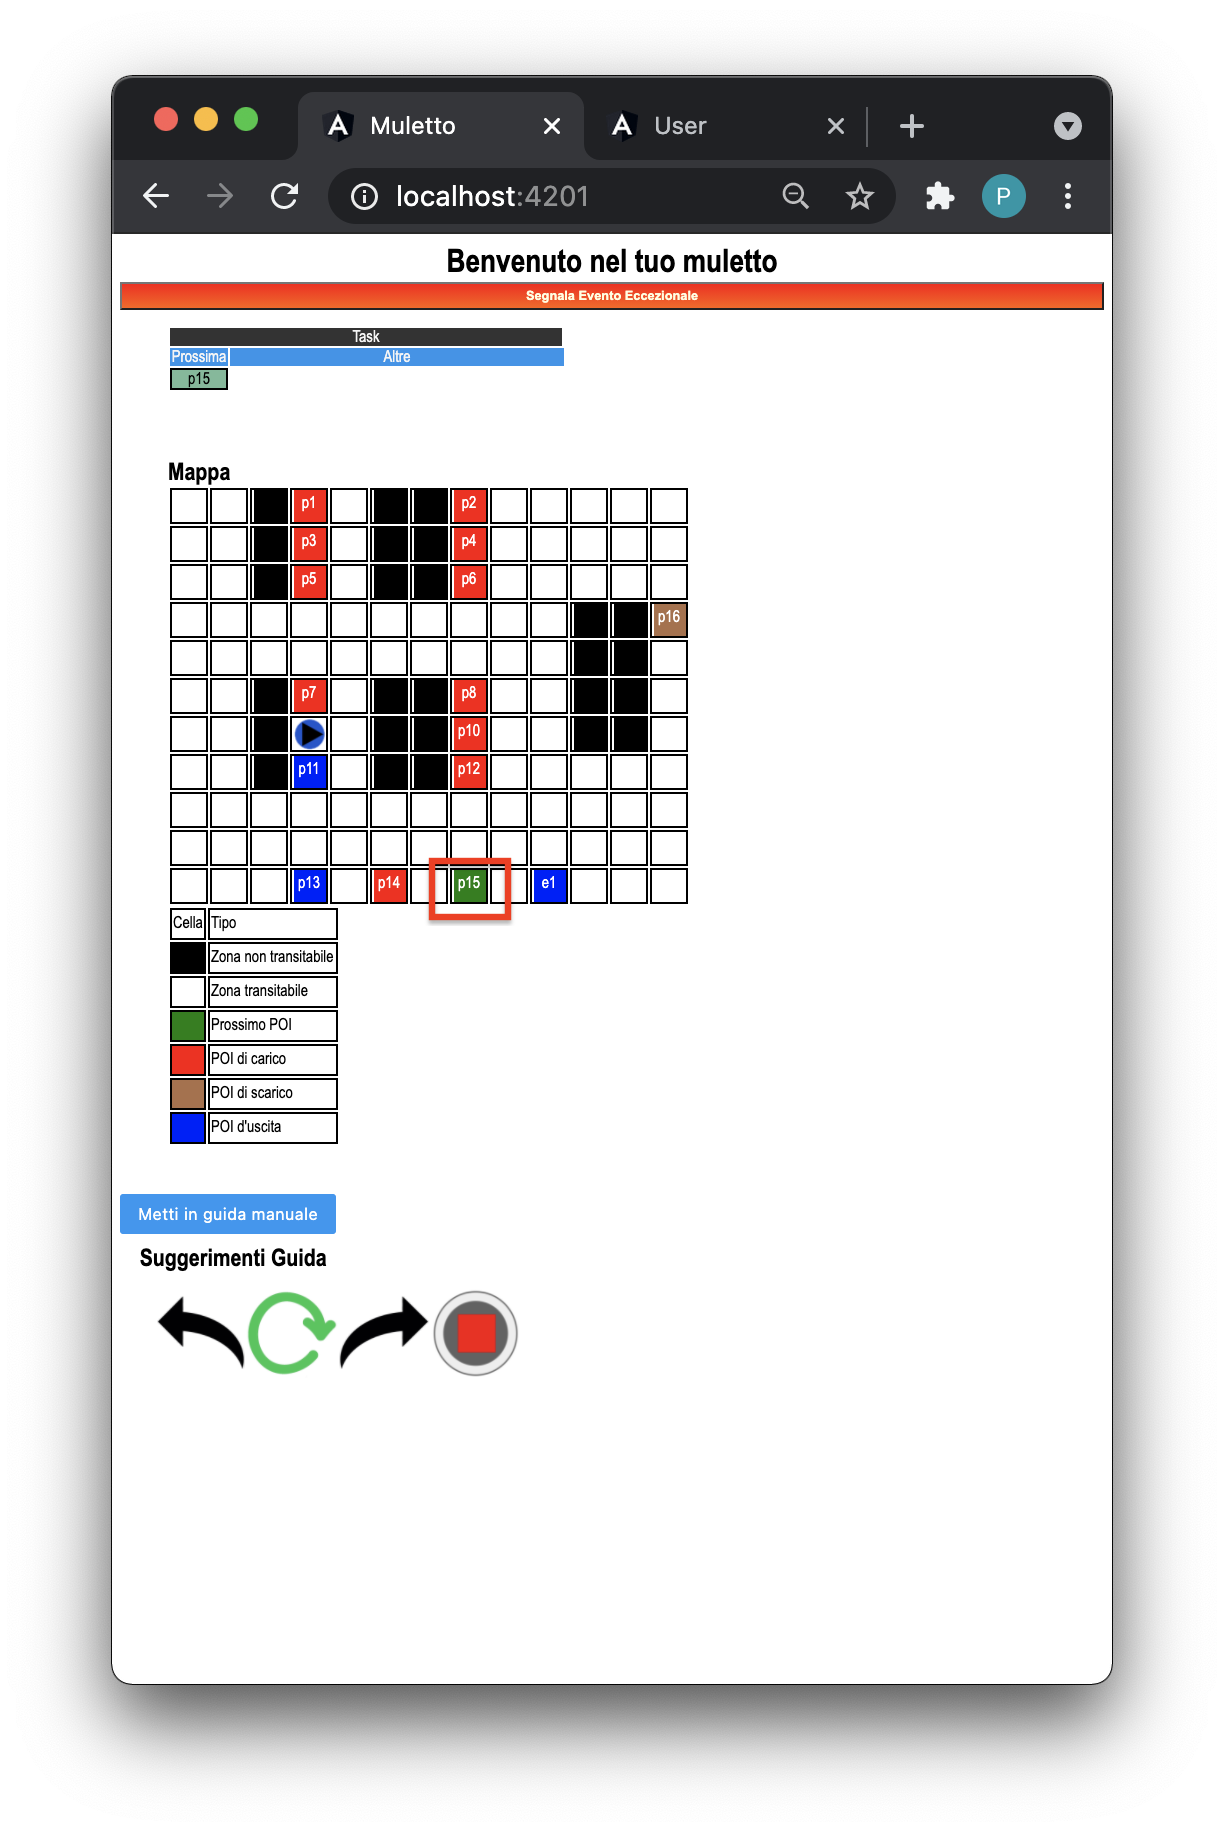
\includegraphics[scale=0.45]{res/images/next.png}
    \end{figure}
\end{itemize}
\subsection{Ritorno alla base}
\begin{itemize}
    \item Quando sono finite le liste di task disponibili, viene visualizzata la base più vicina da raggiungere.
    \item premere il pulsante "Start" per recarsi in essa.
\end{itemize}
\begin{figure}[H]
    \centering
    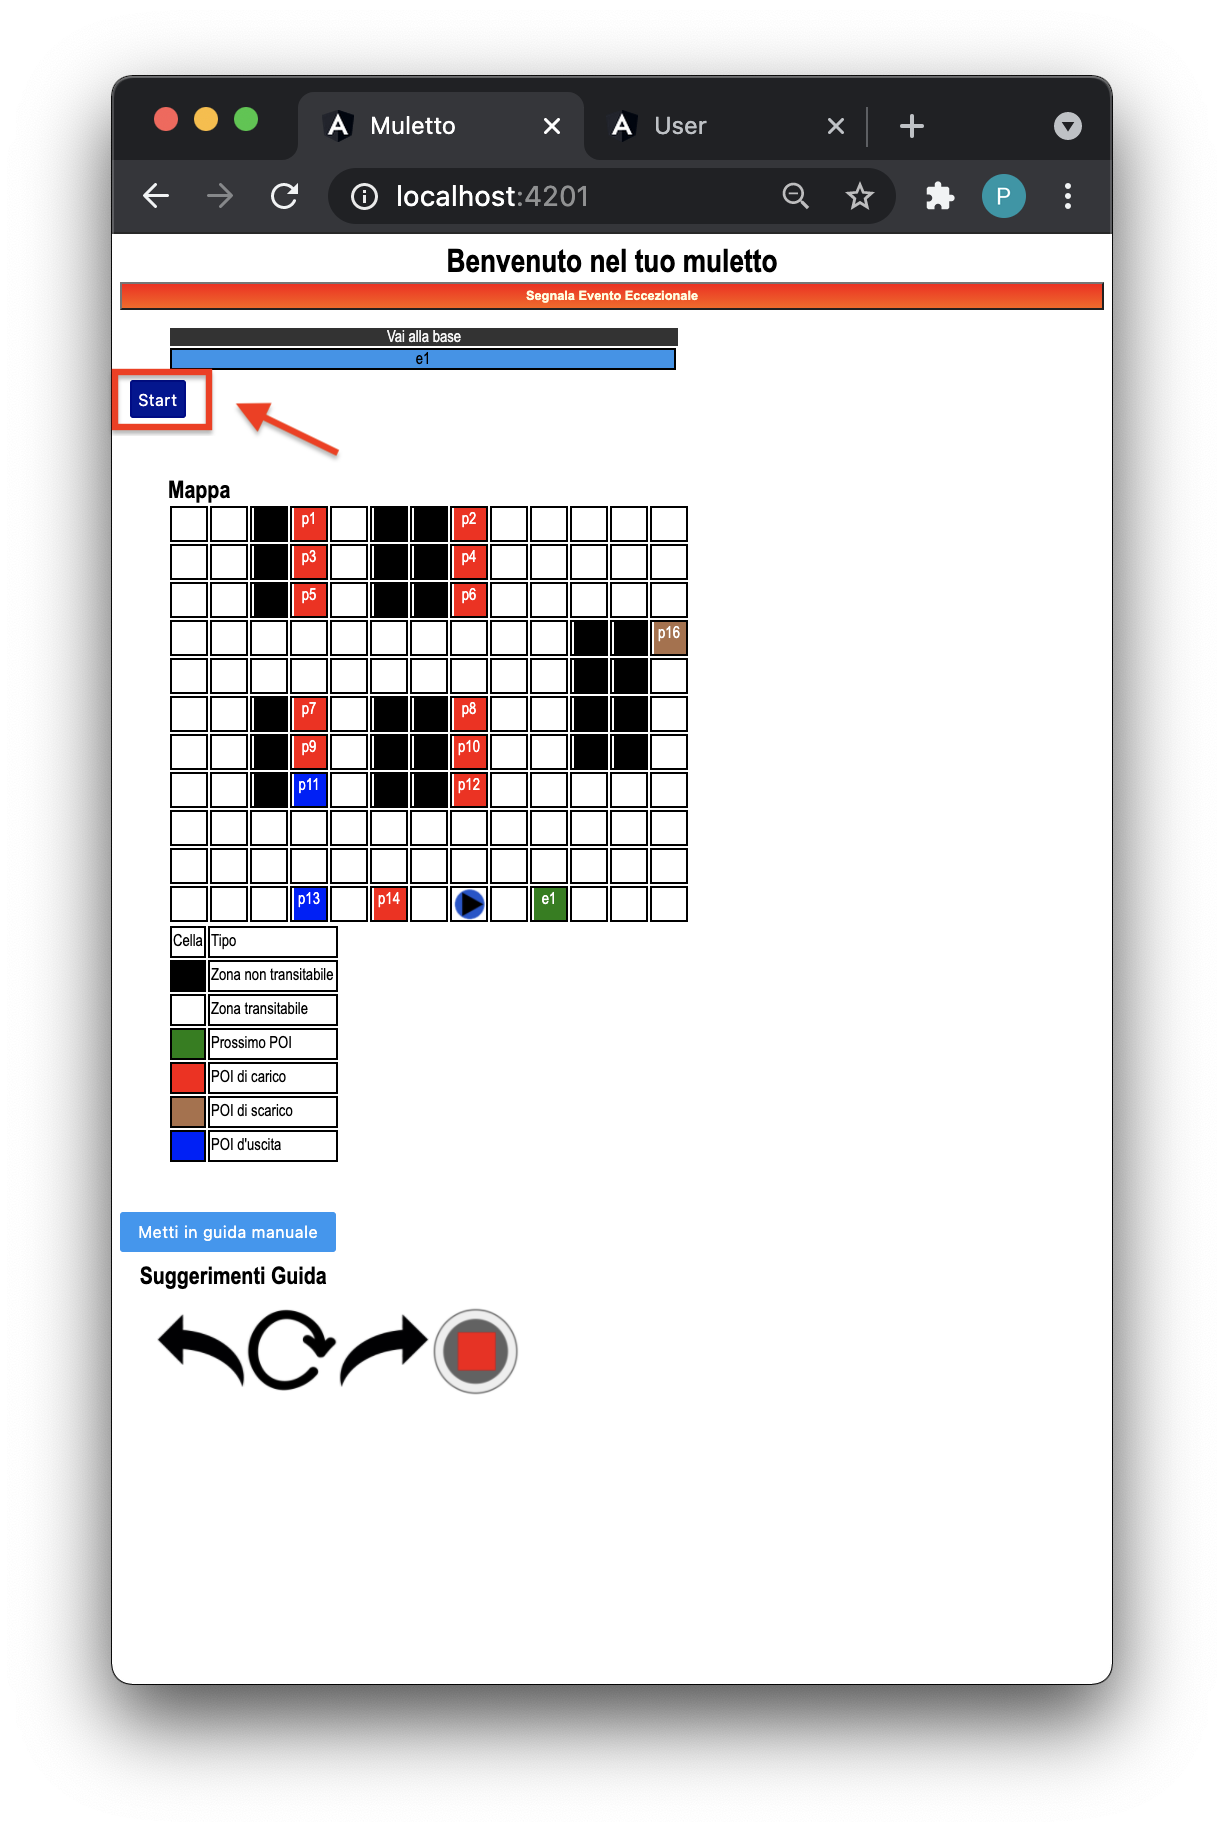
\includegraphics[scale=0.45]{res/images/ritornoallabase.png}
    \caption{Schermata ritorno alla base}
\end{figure}

\subsection{Richiesta nuova lista di task}
\begin{itemize}
    \item Quando ci si trova in base è possibile richiedere una nuova lista di task premendo su "Richiedi nuova lista"
    \begin{figure}[H]
        \centering
        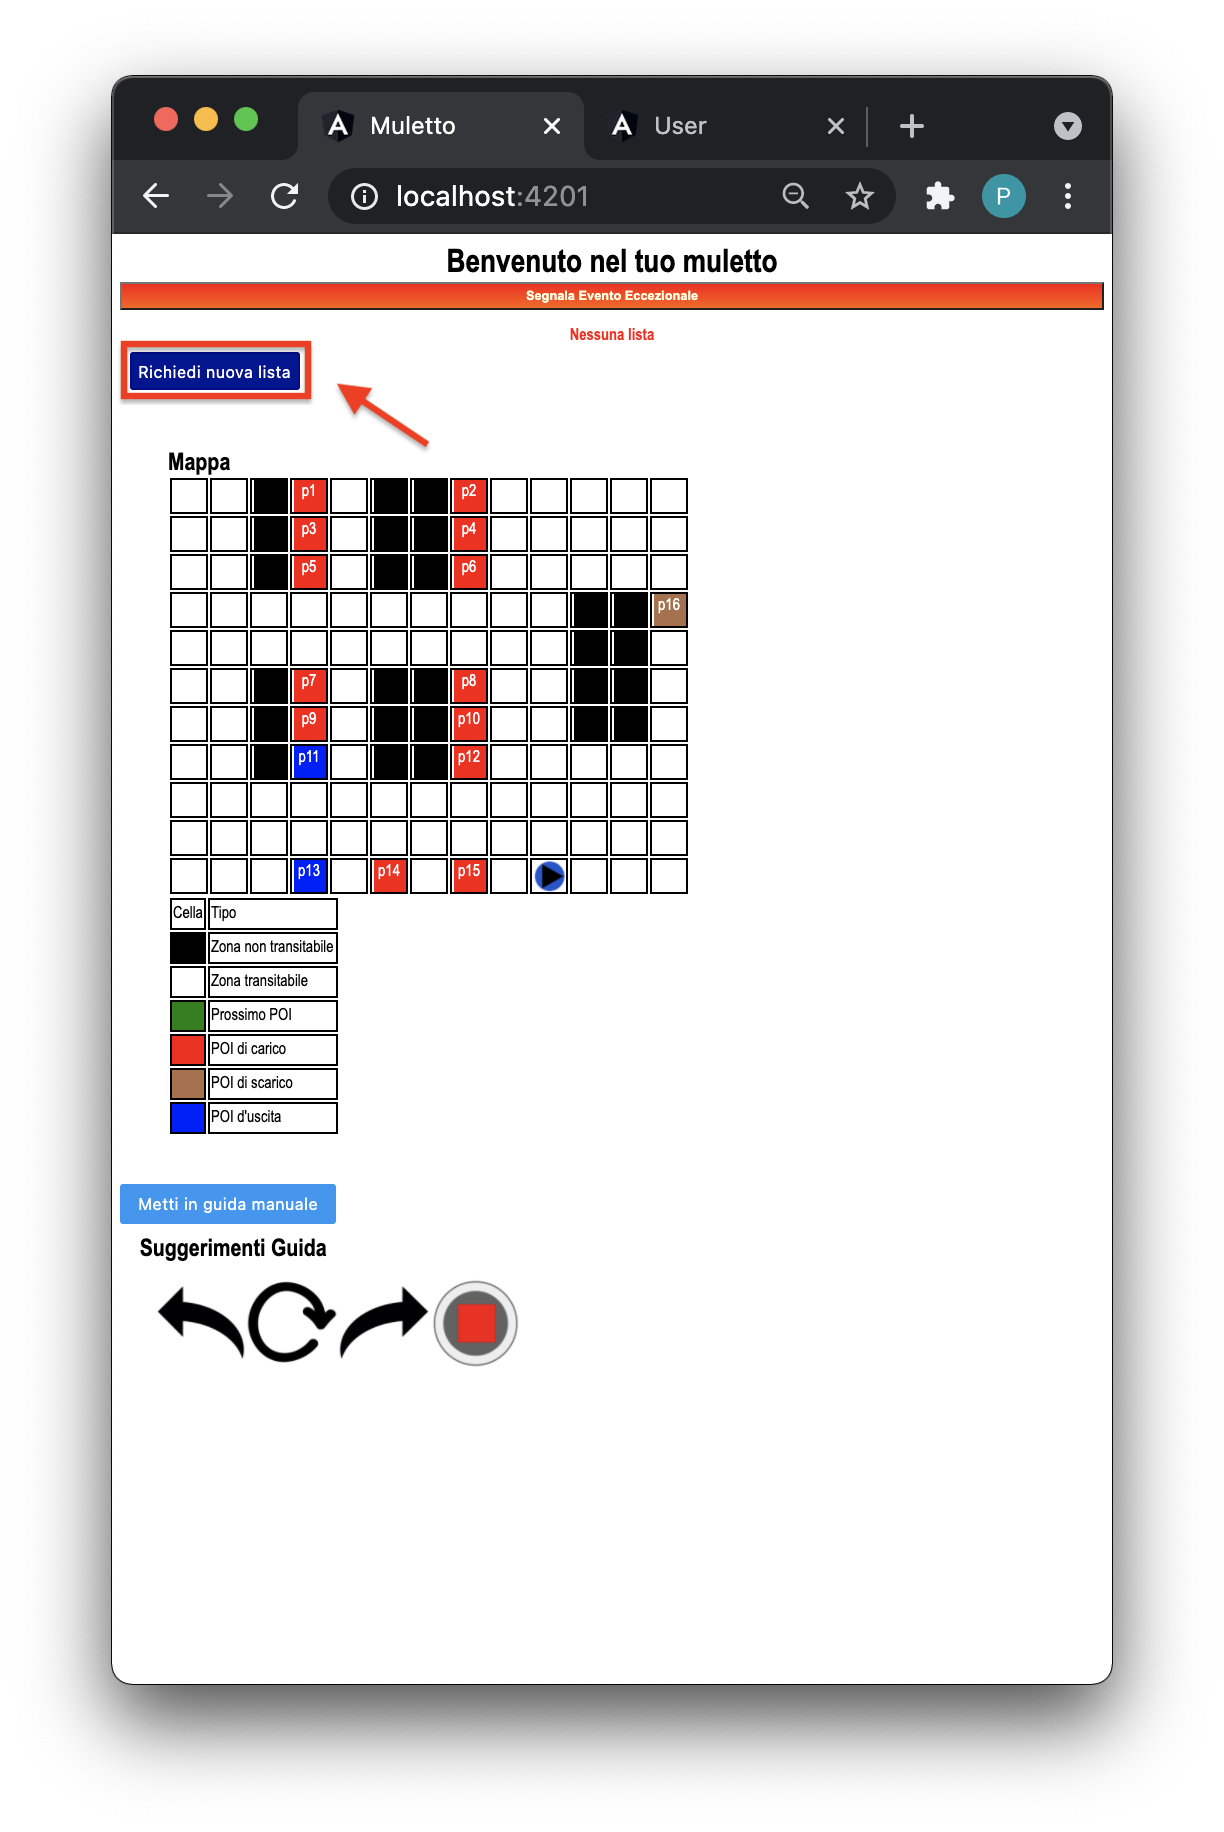
\includegraphics[scale=0.45]{res/images/nuovalista.png}
        \caption{Schermata richiesta nuova lista}
    \end{figure}
    \item se non è presente alcuna lista disponibile bisogna riprovare più tardi.
    \begin{figure}[H]
        \centering
        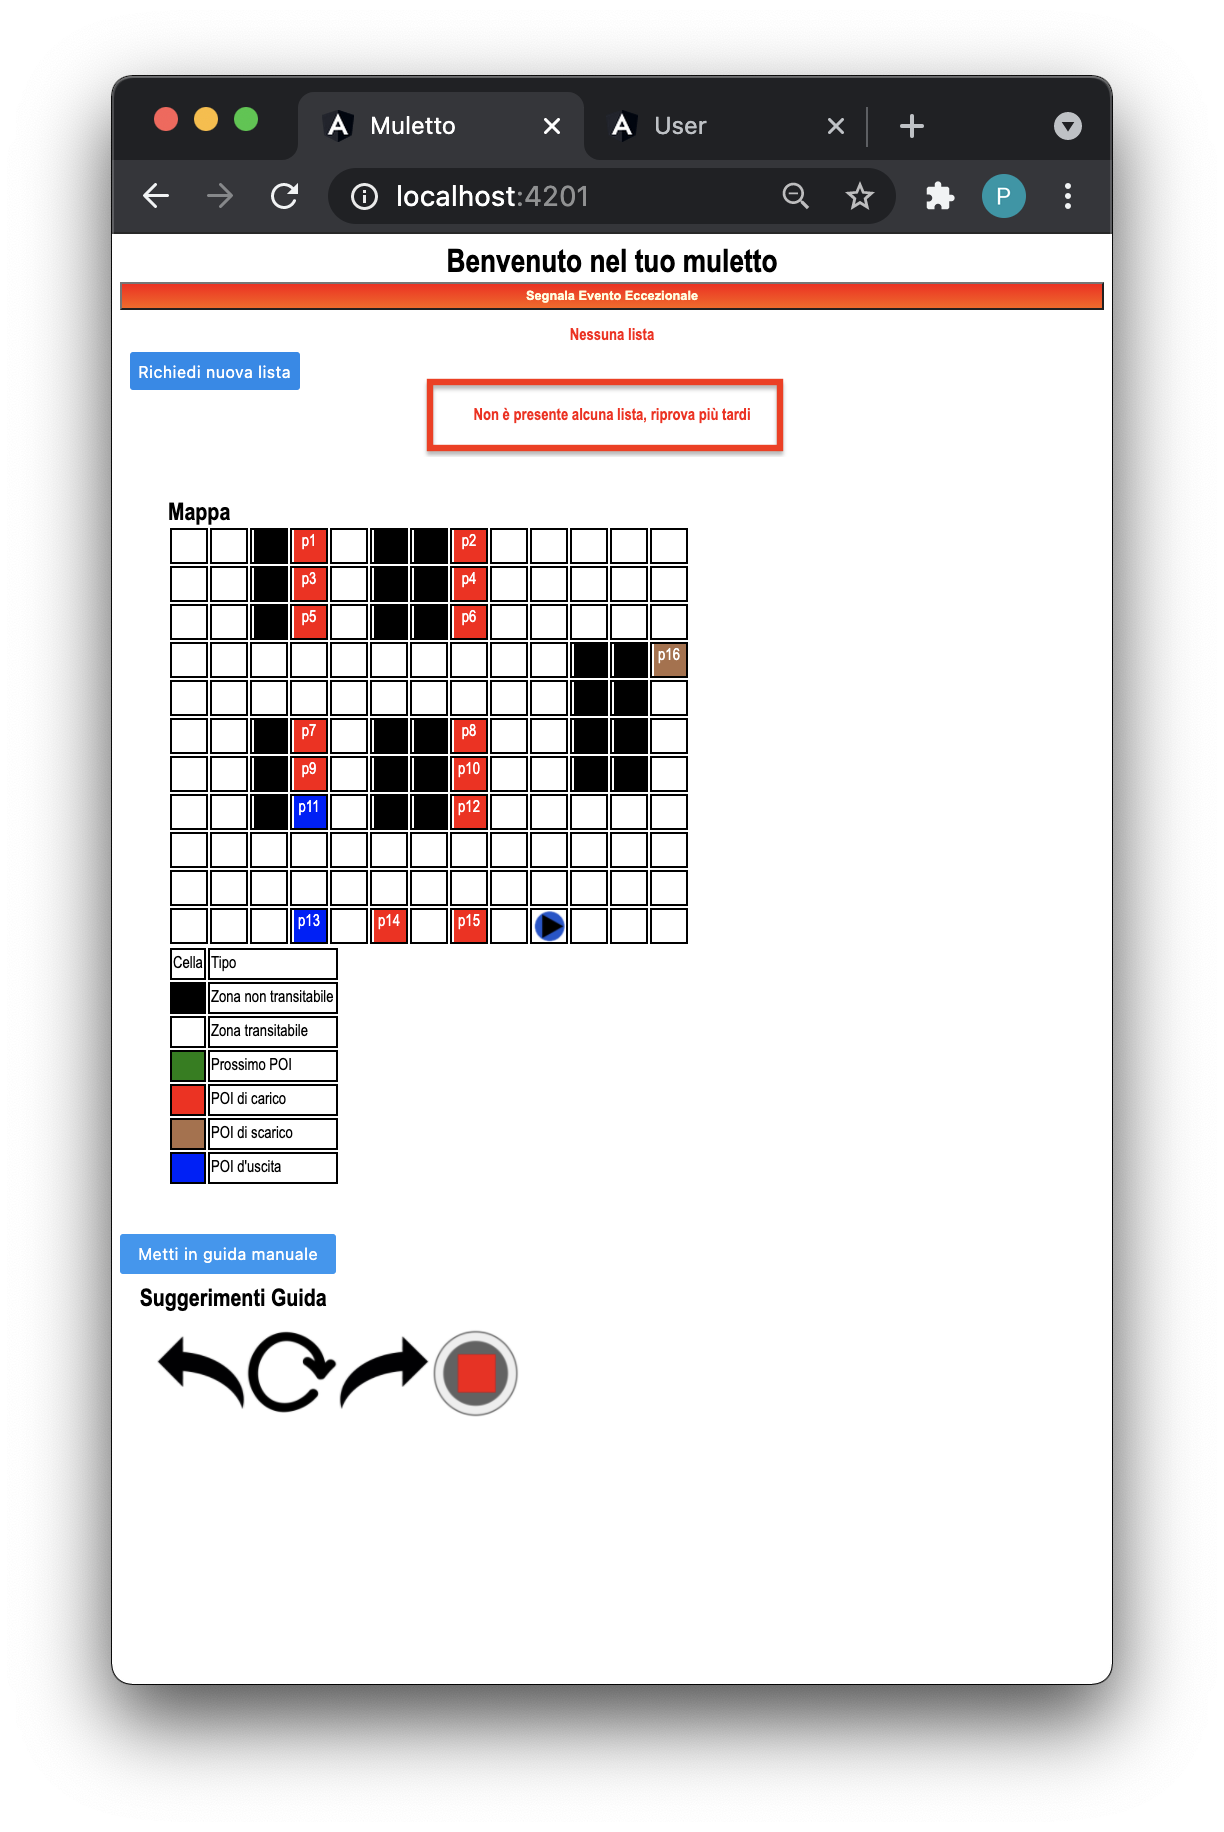
\includegraphics[scale=0.45]{res/images/nolist.png}
        \caption{Schermata nessuna lista disponibile}
    \end{figure}
\end{itemize}



\subsection{Segnalazione evento eccezionale}
\begin{itemize}
    \item Premere sul pulsante "Evento eccezionale" per notificare all'amministratore l'avvenimento di un evento non previsto.
\end{itemize}
\begin{figure}[H]
    \centering
    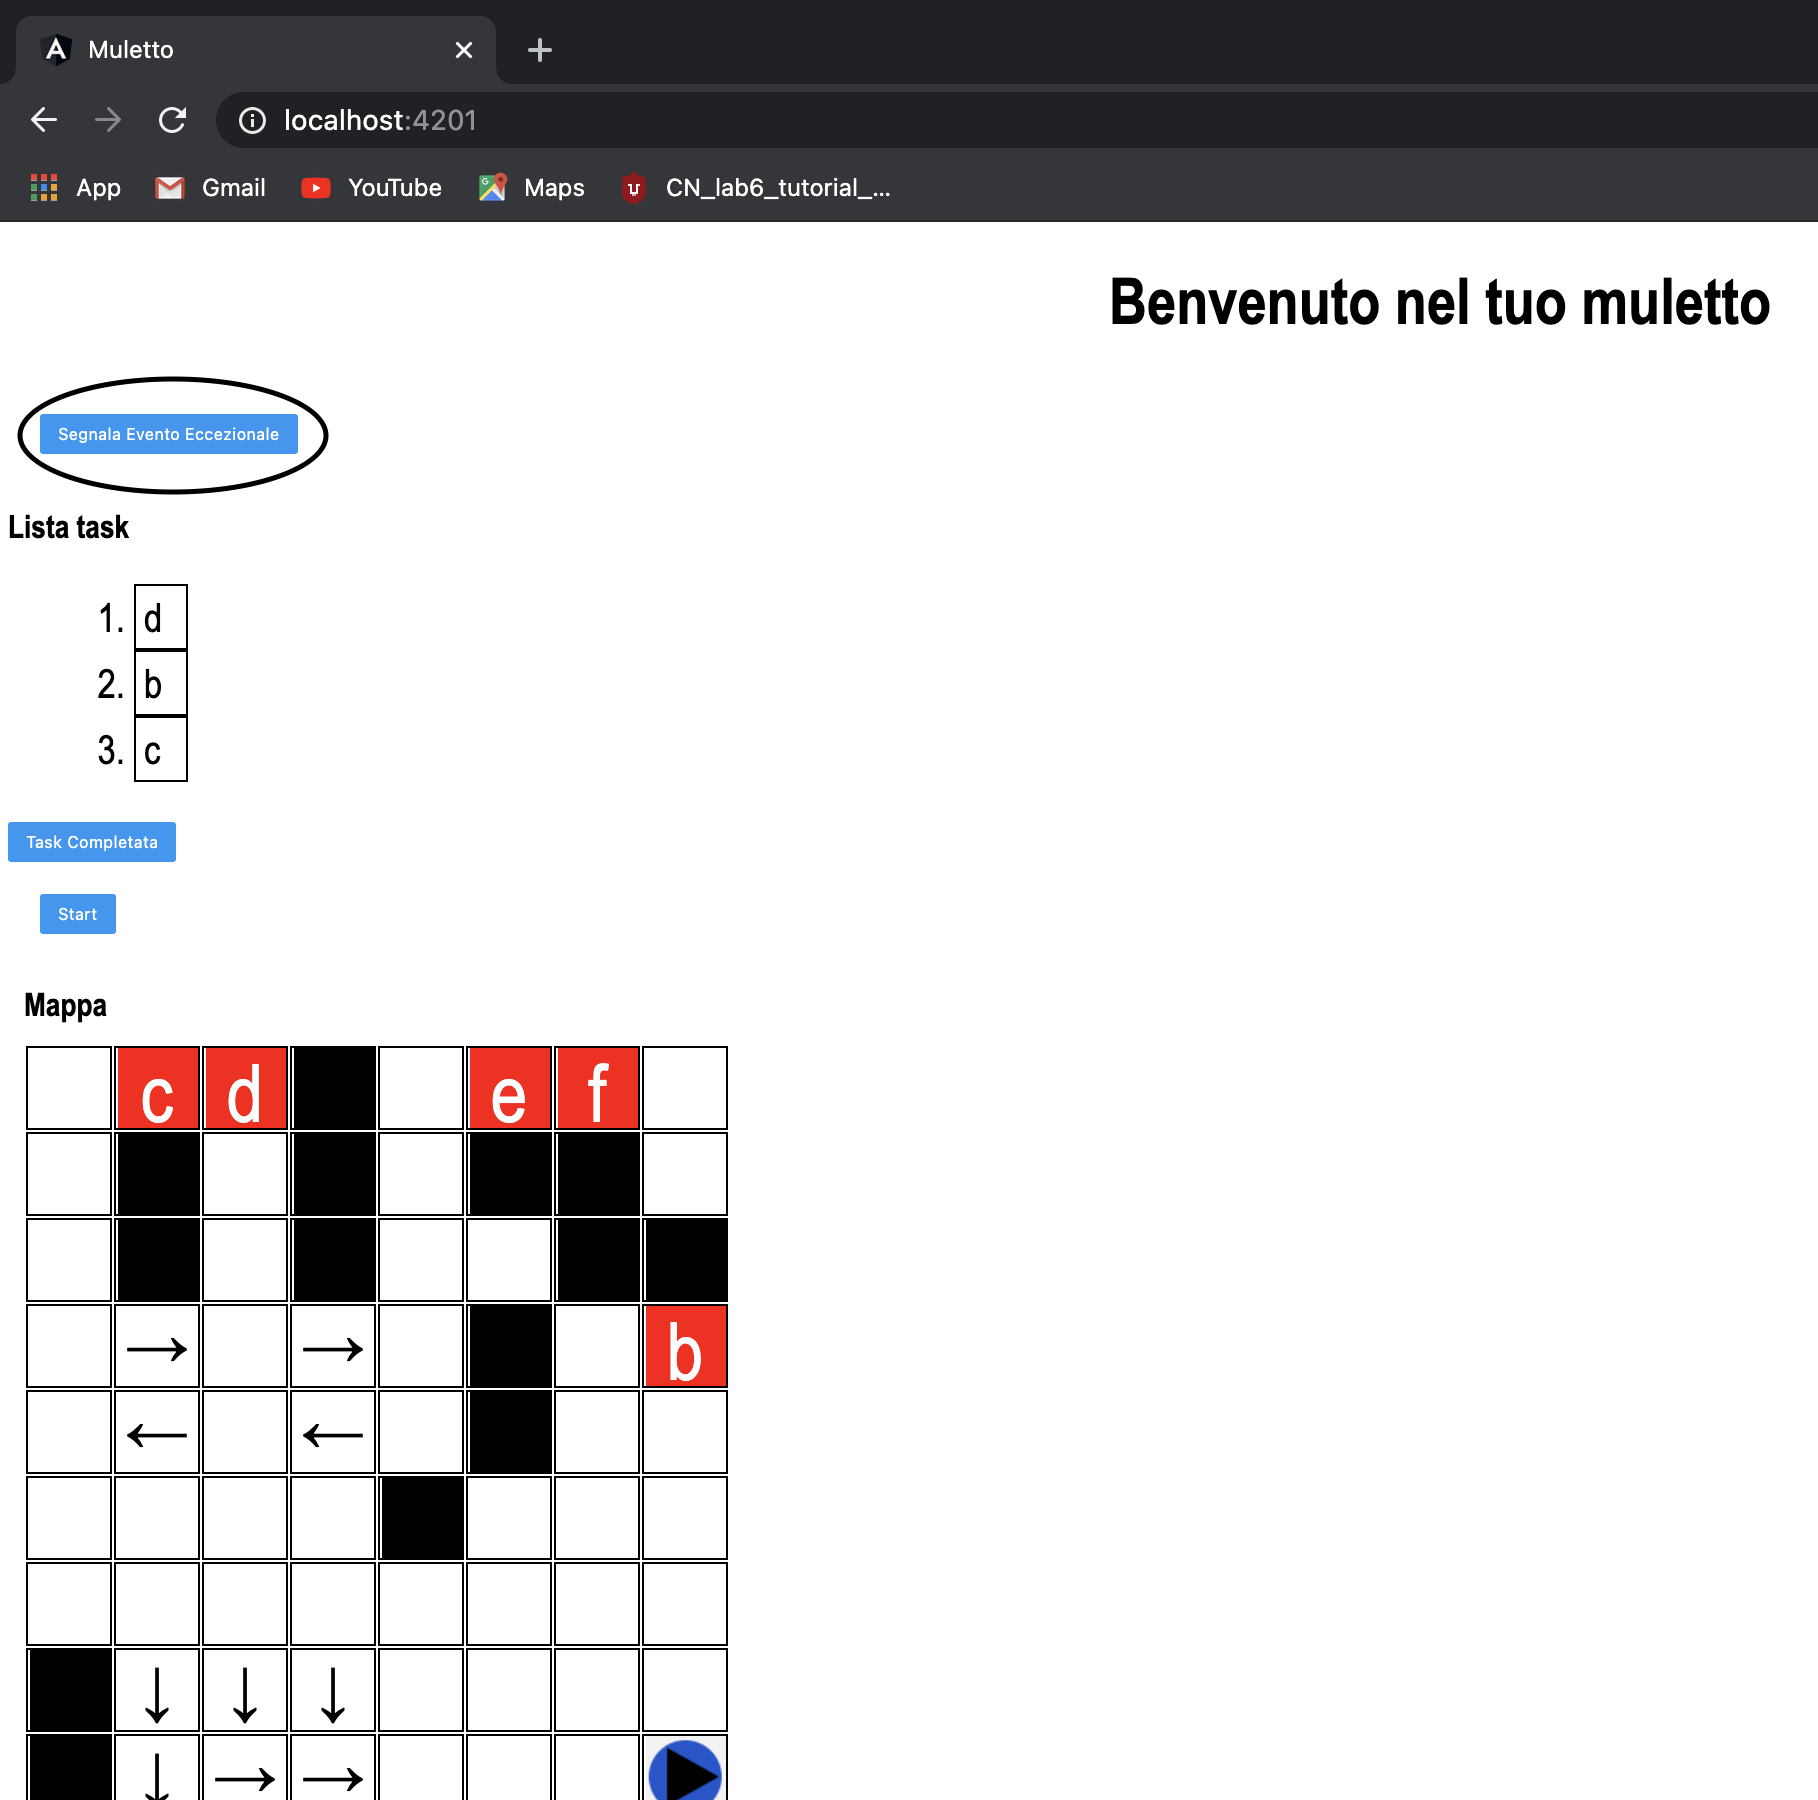
\includegraphics[scale=0.45]{res/images/forklift_evento.png}
    \caption{Schermata segnalazione evento eccezionale}
\end{figure}

	\pagebreak
	
\end{document}
